\documentclass[utf8,secheader]{beamer}
\usepackage[utf8]{inputenc}
\usepackage[russian]{babel}
\usetheme{Madrid}
\addtobeamertemplate{navigation symbols}{}{%
    \usebeamerfont{footline}%
    \usebeamercolor[fg]{footline}%
    \hspace{1em}%
    \insertframenumber/\inserttotalframenumber
}
%\mode<presentation>
%{
  %\usetheme{Madrid}%{Frankfurt}%{Madrid}%{PaloAlto}%{Frankfurt}%{Berkeley}%{Warsaw}%{CambridgeUS}
  %% or ...
%\usecolortheme{seahorse}%{wolverine}%{albatross}%{beaver}%{beetle}%{crane}%{dolphin}%{dove}%{fly}%{lily}%{orchid}%{rose}%{seagull}%{seahorse}%{sidebartab}%{whale}%{wolverine}
  %\setbeamercovered{transparent}
 %\usefonttheme{professionalfonts}
%}
\useoutertheme{shadow}
\title{Ориентационная структура ХЖК ...}
\date{24.12.2019}
\author{Оскирко А. Д.}
% Создание своей теоремы
\newtheorem{MyTheorem}{Теорема}

\usepackage{amssymb}
\usepackage{amsfonts}
\usepackage{amsmath}
\usepackage{graphicx}
\graphicspath{{images/}}
\usepackage{commath}
\usepackage{euscript}

\newcommand\blfootnote[1]{%
  \begingroup
  \renewcommand\thefootnote{}\footnote{#1}%
  \addtocounter{footnote}{-1}%
  \endgroup
}

\renewcommand{\tilde}[1]{\widetilde{#1}}
\renewcommand{\le}{\leqslant}
\renewcommand{\ge}{\geqslant}
\newcommand{\norma}[1]{\left \| #1 \right \|}
\newcommand{\pder}[2]{\frac{\partial {#1}}{\partial {#2}}}
\newcommand{\pdder}[2]{\frac{\partial^2 {#1}}{\partial {#2}^2}}\usepackage{mathrsfs}\usepackage{placeins}\usepackage{empheq}\renewcommand{\phi}{\varphi}\newcommand*\widefbox[1]{\fbox{\hspace{1em}#1\hspace{1em}}}
\DeclareMathOperator*{\diag}{diag}
\DeclareMathOperator*{\rot}{rot}
\DeclareMathOperator*{\diver}{div}
\DeclareMathOperator*{\grad}{grad}
\DeclareMathOperator*{\supp}{\mathbf{supp}}
\DeclareMathOperator*{\Int}{\mathbf{Int}}
\DeclareMathOperator*{\Ext}{\mathbf{Ext}}\newcommand{\bb}[1]{\textbf{#1}}
\DeclareMathOperator{\sgn}{sgn}
\newcommand{\FF}{\mathcal{F}}
\renewcommand{\AA}{\mathcal{A}}
\newcommand{\BB}{\mathcal{B}}
\newcommand{\CC}{\mathcal{C}}
\newcommand{\DD}{\mathcal{D}}
\newcommand{\EE}{\mathcal{E}}
\newcommand{\II}{\mathcal{I}}
\renewcommand{\epsilon}{\varepsilon}
\renewcommand{\phi}{\varphi}


\setbeamertemplate{caption}[numbered]

\newboolean{showMascot}
\setboolean{showMascot}{false} % boolvar=true or false
\usepackage[absolute,overlay]{textpos}




\newcommand\mktitleframe{%
\begin{frame}% very custom titlepage
\thispagestyle{empty}%
%
\begin{center}%
%

\includegraphics[height=1.5cm]{orel}\\%
{\small\bf Кафедра статистической физики}%

\begin{center}%
\typeofthis
\end{center}%
\vspace{-4mm}%
\begingroup%
\setbeamercolor{block body}{bg=blue!60!black,fg=white}
\begin{block}{}\begin{center}%
\Large\bf\titletext%
\end{center}\end{block}%
\endgroup%
\vfill%
~\par%
\begin{columns}%
\begin{column}{0.33\textwidth}%
\ifthenelse {\boolean{showMascot}}%
{%
\begin{textblock*}{4cm}(0mm,60mm)%
\end{textblock*}%
}{}\end{column}%
\begin{column}{0.67\textwidth}%
{\small\bf Автор:}\\%
\hspace{0.4cm}{\large\authorname}%
\par%
{\small\bf Научный руководитель:}\\%
\hspace{0.4cm}{\large\adviser}%
\par%
%{\small\bf Рецензент:}\\%
%\hspace{0.4cm}{\large\reviewer}%
\end{column}%
\end{columns}%
\par\vspace{0.5cm}%
\speechdate%
\end{center}%
\end{frame}%
}

\begin{document}






\def\typeofthis{}%Квалификационная работа\\бакалавра информационных технологий}
\def\titletext{Исследование изменения ориентационной структуры 	кирального жидкого кристалла с большим флексоэлектрическим коэффициентом под воздействием внешнего электрического поля
}
\def\authorname{Оскирко А.Д.}
\def\adviser{д. ф.-м.н., проф. %$|$ 
Ульянов С. В.}
%\def\reviewer{д. ф.-м.н., проф. $|$ Ульянов С. В.}
%\def\adviser{д.~ф.-м.н., проф. $|$ Романов В. П.}
\def\speechdate{Санкт-Петербург, 2020~г.}

\mktitleframe





\begin{frame}[t]
\frametitle{Содержание}

\begin{enumerate}
	\item Свободная энергия искажения ориентационной структуры ХЖК
%\item \alert{Статья PRE2018 ? а Journal of Physics 2 шт?}
	\item Переход Фредерикса в случае отрицательной анизотропии диэлектрической проницаемости
	\item Переход между искажёнными ориентационными структурами в случае большого усреднённого флексоэлектрического коэффициента
\end{enumerate}
\end{frame}



%
%\begin{frame}[t]
%\frametitle{Постановка задачи}
%Рассматриваемая система:
%\begin{figure}[ht]
%\centering
%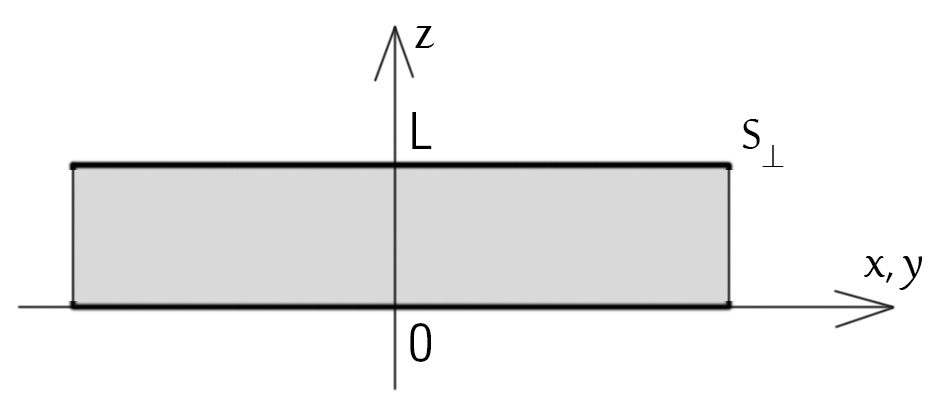
\includegraphics[width=9cm]{pic1}
%\caption{Ячейка ХЖК}
%\end{figure}
%\FloatBarrier
%\end{frame}

\begin{frame}
\centering
{\large Часть 1. Свободная энергия искажения ориентационной структуры ХЖК.}%\blfootnote{Результаты опубликованы в статье \textit{A.~D.~Oskirko, S.~V.~Ul'yanov and A.~Yu.~Val'kov} \textbf{Influence of flexoelectric effect on the Fréedericksz transition in chiral nematic liquid crystals} Physical Review E 98, 012702 (2018)}}%, DOI:~10.1103/PhysRevE.98.012702}}
\end{frame}

\begin{frame}[t]
\frametitle{Описание системы}
\begin{minipage}{0.49\textwidth}
\begin{figure}[ht]
\centering
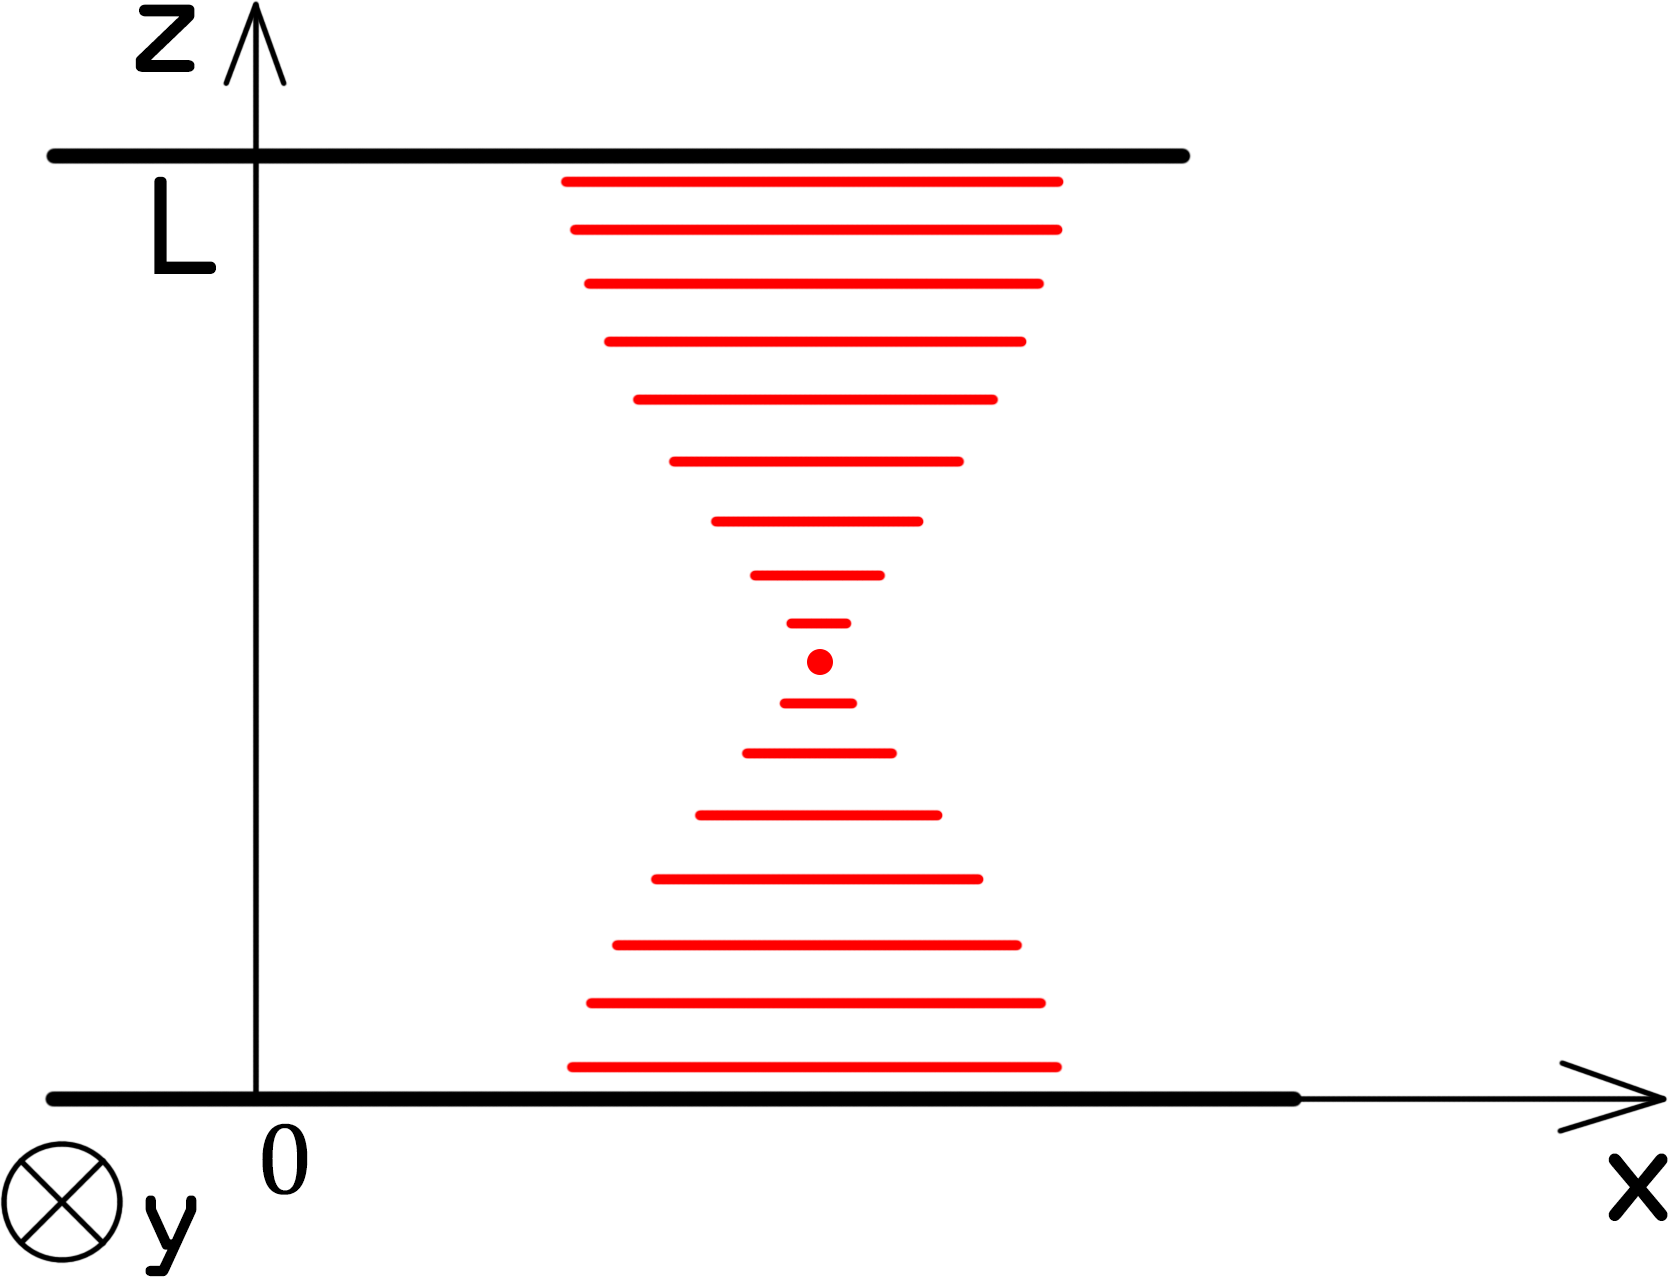
\includegraphics[width=\textwidth]{decart.png}
\caption{Планарная геликоидальная структура ХЖК}
\end{figure}
\end{minipage}
\hfill
\begin{minipage}{0.49\textwidth}
\begin{figure}[ht]
\centering
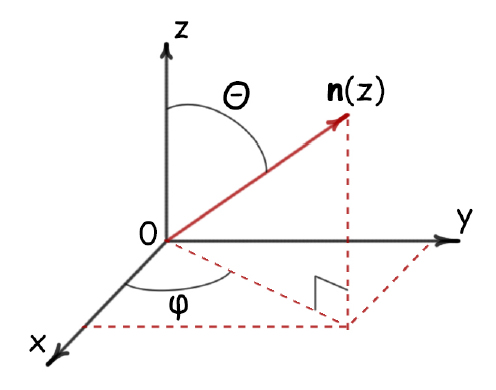
\includegraphics[width=\textwidth]{pic_04.jpg}
\caption{Ориентация директора  $\mathbf{n}$}
\end{figure}
\end{minipage}
\end{frame}





%\begin{frame}
%\frametitle{Постановка задачи}


%\begin{figure}[ht]
%\centering
%\begin{minipage}{0.49\textwidth}
%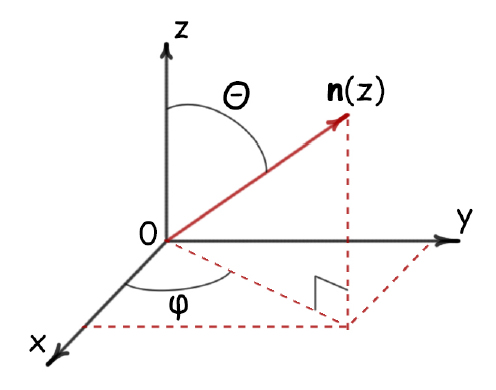
\includegraphics[width=\textwidth]{pic2}
%\end{minipage}
%\hfil
%\begin{minipage}{0.49\textwidth}
%$$
%\begin{cases}
% &n_x = \sin{\theta} \cos{\phi} \\
% &n_y = \sin{\theta} \sin{\phi} \\
% &n_z = \cos{\theta}
%\end{cases}
%$$
%\end{minipage}
%\caption{Сферические координаты директора}
%\end{figure}
%\FloatBarrier
%\end{frame}%

%
%\begin{frame}
%\frametitle{Флексоэлектрическая поляризация}
%\begin{figure}[ht]
%\centering
%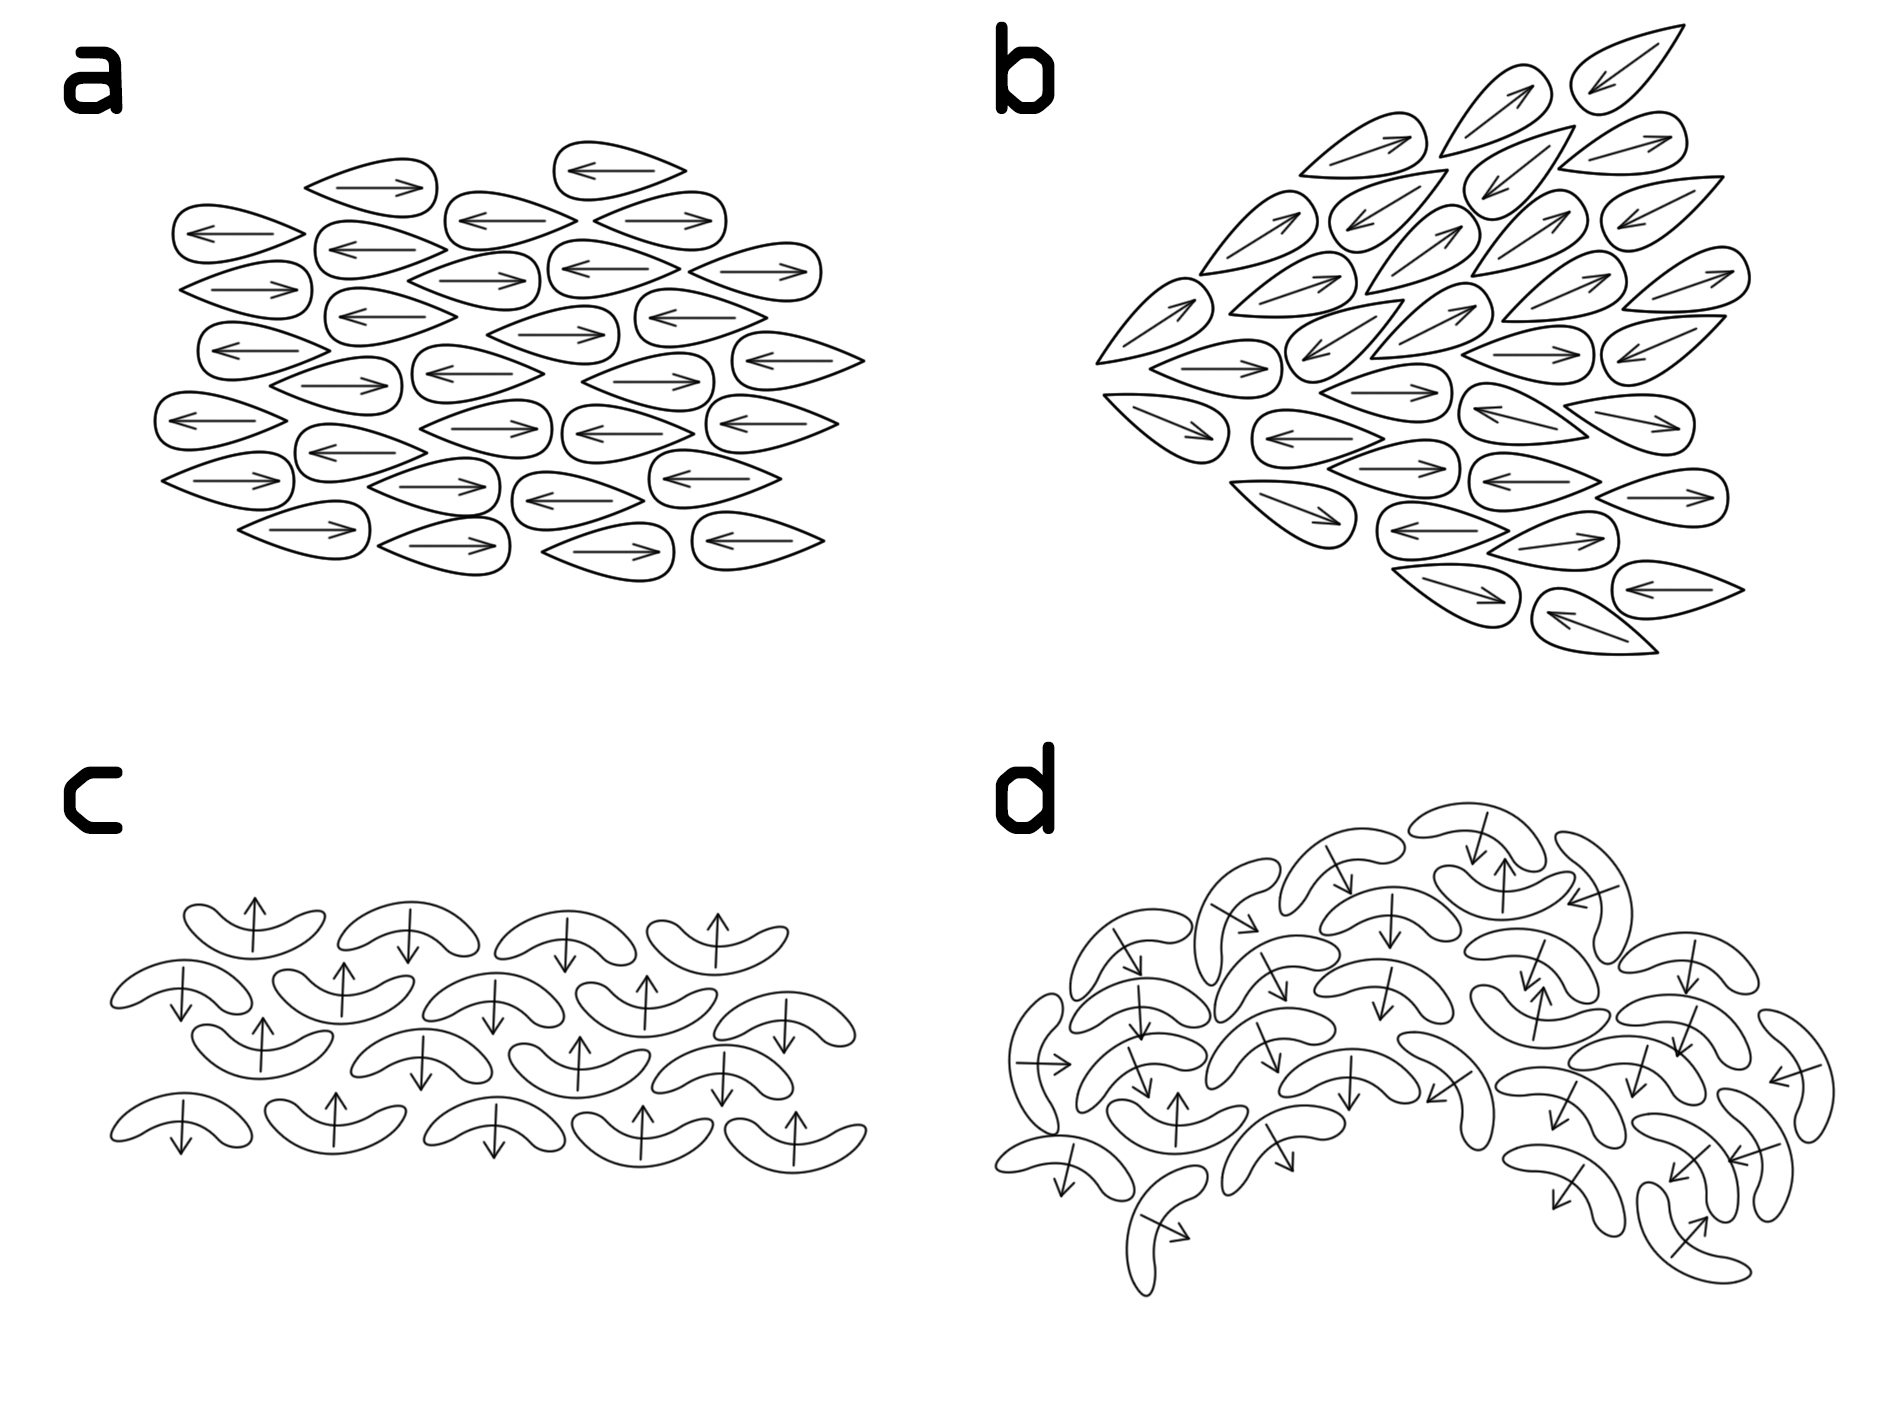
\includegraphics[width=10cm]{Molecules}
%\end{figure}
%\FloatBarrier
%\end{frame}
%
%\begin{frame}
%\frametitle{Флексоэлектрическая поляризация}
%\begin{figure}[ht]
%\centering
%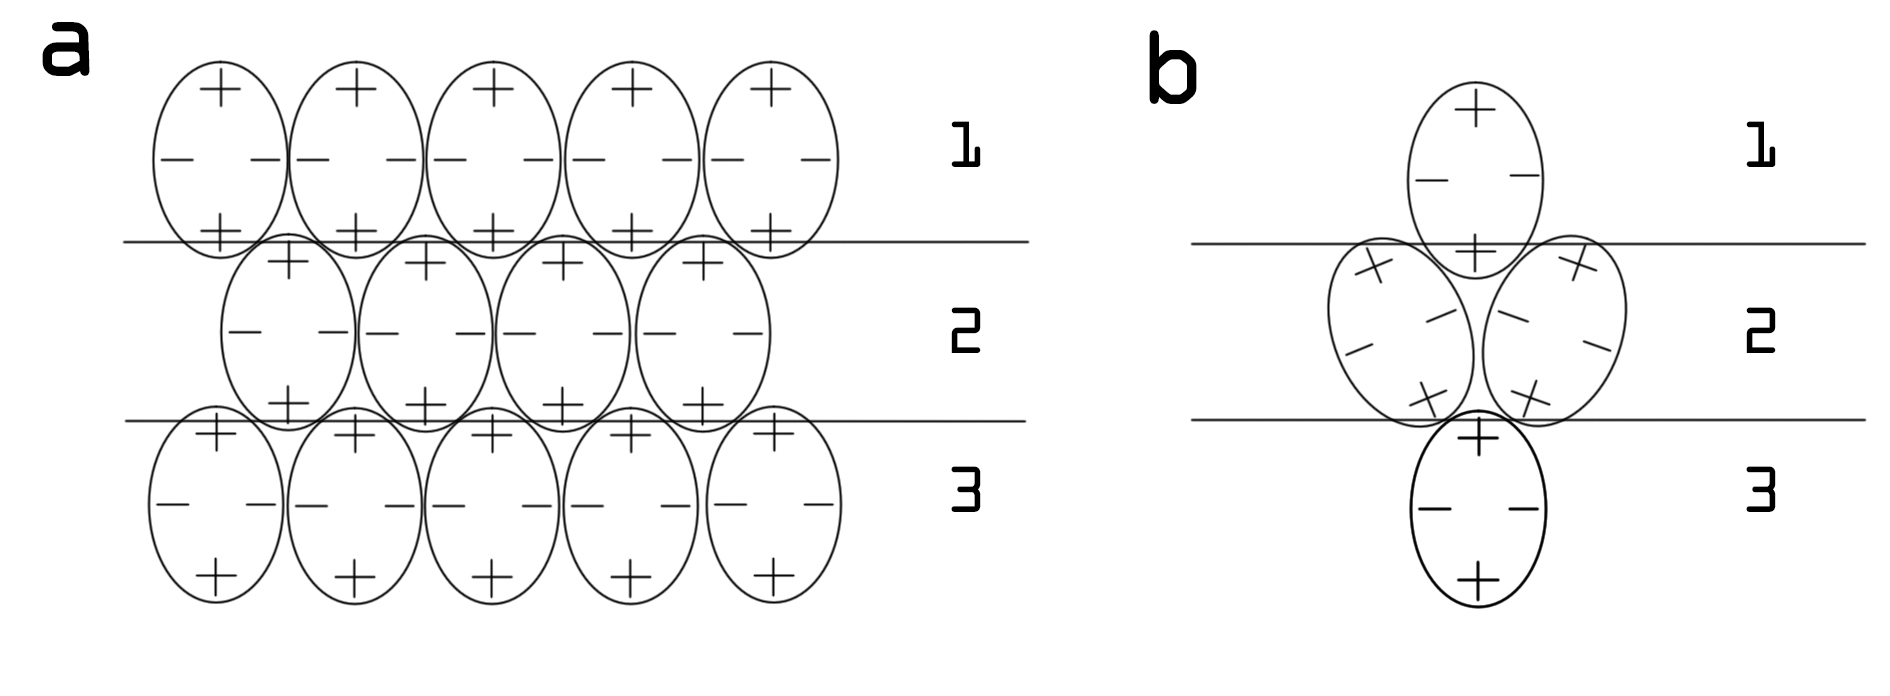
\includegraphics[width=12cm]{Prost_explanation}
%\end{figure}
%\FloatBarrier
%\end{frame}







\begin{frame}
\frametitle{Свободная энергия ХЖК во внешнем поле}
\begin{block}{Общий вид выражения}
\begin{equation}
\FF_\mathrm{tot} = \FF_\mathrm{e} + \FF_\mathrm{sf} + \FF_\mathrm{f}% + \FF_\mathrm{flex}
\label{eq1}
\end{equation}
\end{block}
\only<2>{
\begin{block}{Упругая энергия}
\footnotesize
\begin{align}\label{eq:F_e_from_n}
&\FF_e = \frac{S_{\!\bot}}{2} \int_0^L\left[ K_{11} (\diver{\bf n})^2+K_{22} ({\bf n}\cdot\rot{{\bf n}} + q_0)^2 + K_{33} ({\bf n}\times \rot{{\bf n}})^2 \right]\, dz, \\
&\FF_\mathrm{sf} =  \frac{S_\perp}{2}\sum\limits_{\alpha=1,2} \left[W_\theta^{(\alpha)} \sin^2{\left( \theta - \theta_0^{(\alpha)} \right)} + W_\phi^{(\alpha)} \sin^2{\left( \phi - \phi_0^{(\alpha)} \right)}\right]
\end{align}
\end{block}
}
\only<3>{
\begin{block}{Вклад флексоэлектричества}
\begin{equation}\label{FF_f_basic}
\mathcal{F}_{f}=\int_V F_{f}\,d{\bf r},\; F_{f}=-\frac{1}{4\pi }\int \mathbf{D} d\mathbf{E},
\end{equation}
%where ${\bf E}$ is the electric, and  ${\bf D}$ is the displacement fields~\cite{LLECM, deGennesbook1995}. In the presence of flexoelectricity the electric displacement field takes the form
\begin{equation}\label{eq_material}
\mathbf{D}=\hat\varepsilon \mathbf{E}+4\pi \mathbf{P}_\text{flex},
\end{equation}
\begin{equation}\label{FF_f_basic1}
 \FF_{f} = -\frac{S_{\!\bot}}{8\pi} \int_0^L {\bf E}\cdot\hat{\varepsilon}{\bf E}\, dz -{S_{\!\bot}}\int_0^L{\bf P}_{\mathrm{flex}}\cdot {\bf E} \, dz
\end{equation}
\begin{eqnarray}
&\varepsilon_{\alpha\beta}=\varepsilon_\bot \delta_{\alpha\beta}+\varepsilon_a n_\alpha n_\beta,\label{eq2_0}\\
&\mathbf{P}_\text{flex}=e_1{\bf n}\diver {\bf n}+e_3\rot{\bf n}\times{\bf n},\label{eq2}
\end{eqnarray}
\end{block}
}
\only<4>{
\begin{block}{Результат}
\begin{equation}\label{eq_F_f_final1}
\FF_{f}=-\frac{S_{\!\bot}}{8\pi}U^2 J +S_{\!\bot} \bar{e}_{13}U JJ_1+2\pi S_{\!\bot} \bar{e}_{13}^2\left(\int_{0}^{L}\frac{(\sin 2\theta \,\theta')^2}{{\EE}(\theta)}dz -JJ_1^2\right)
\end{equation}
$$
J_1=\ln{\frac{\EE(\theta(0))}{\EE(\theta(L))}},\quad J = \left( \int\limits_0^L \frac{1}{\EE(\theta)}\,dz \right)^{-1}\hspace{-0.5cm},\quad \EE(\theta) = \epsilon_\perp + \epsilon_a \cos^2(\theta)
$$
\end{block}
}
%\begin{figure}[ht]
%\centering
%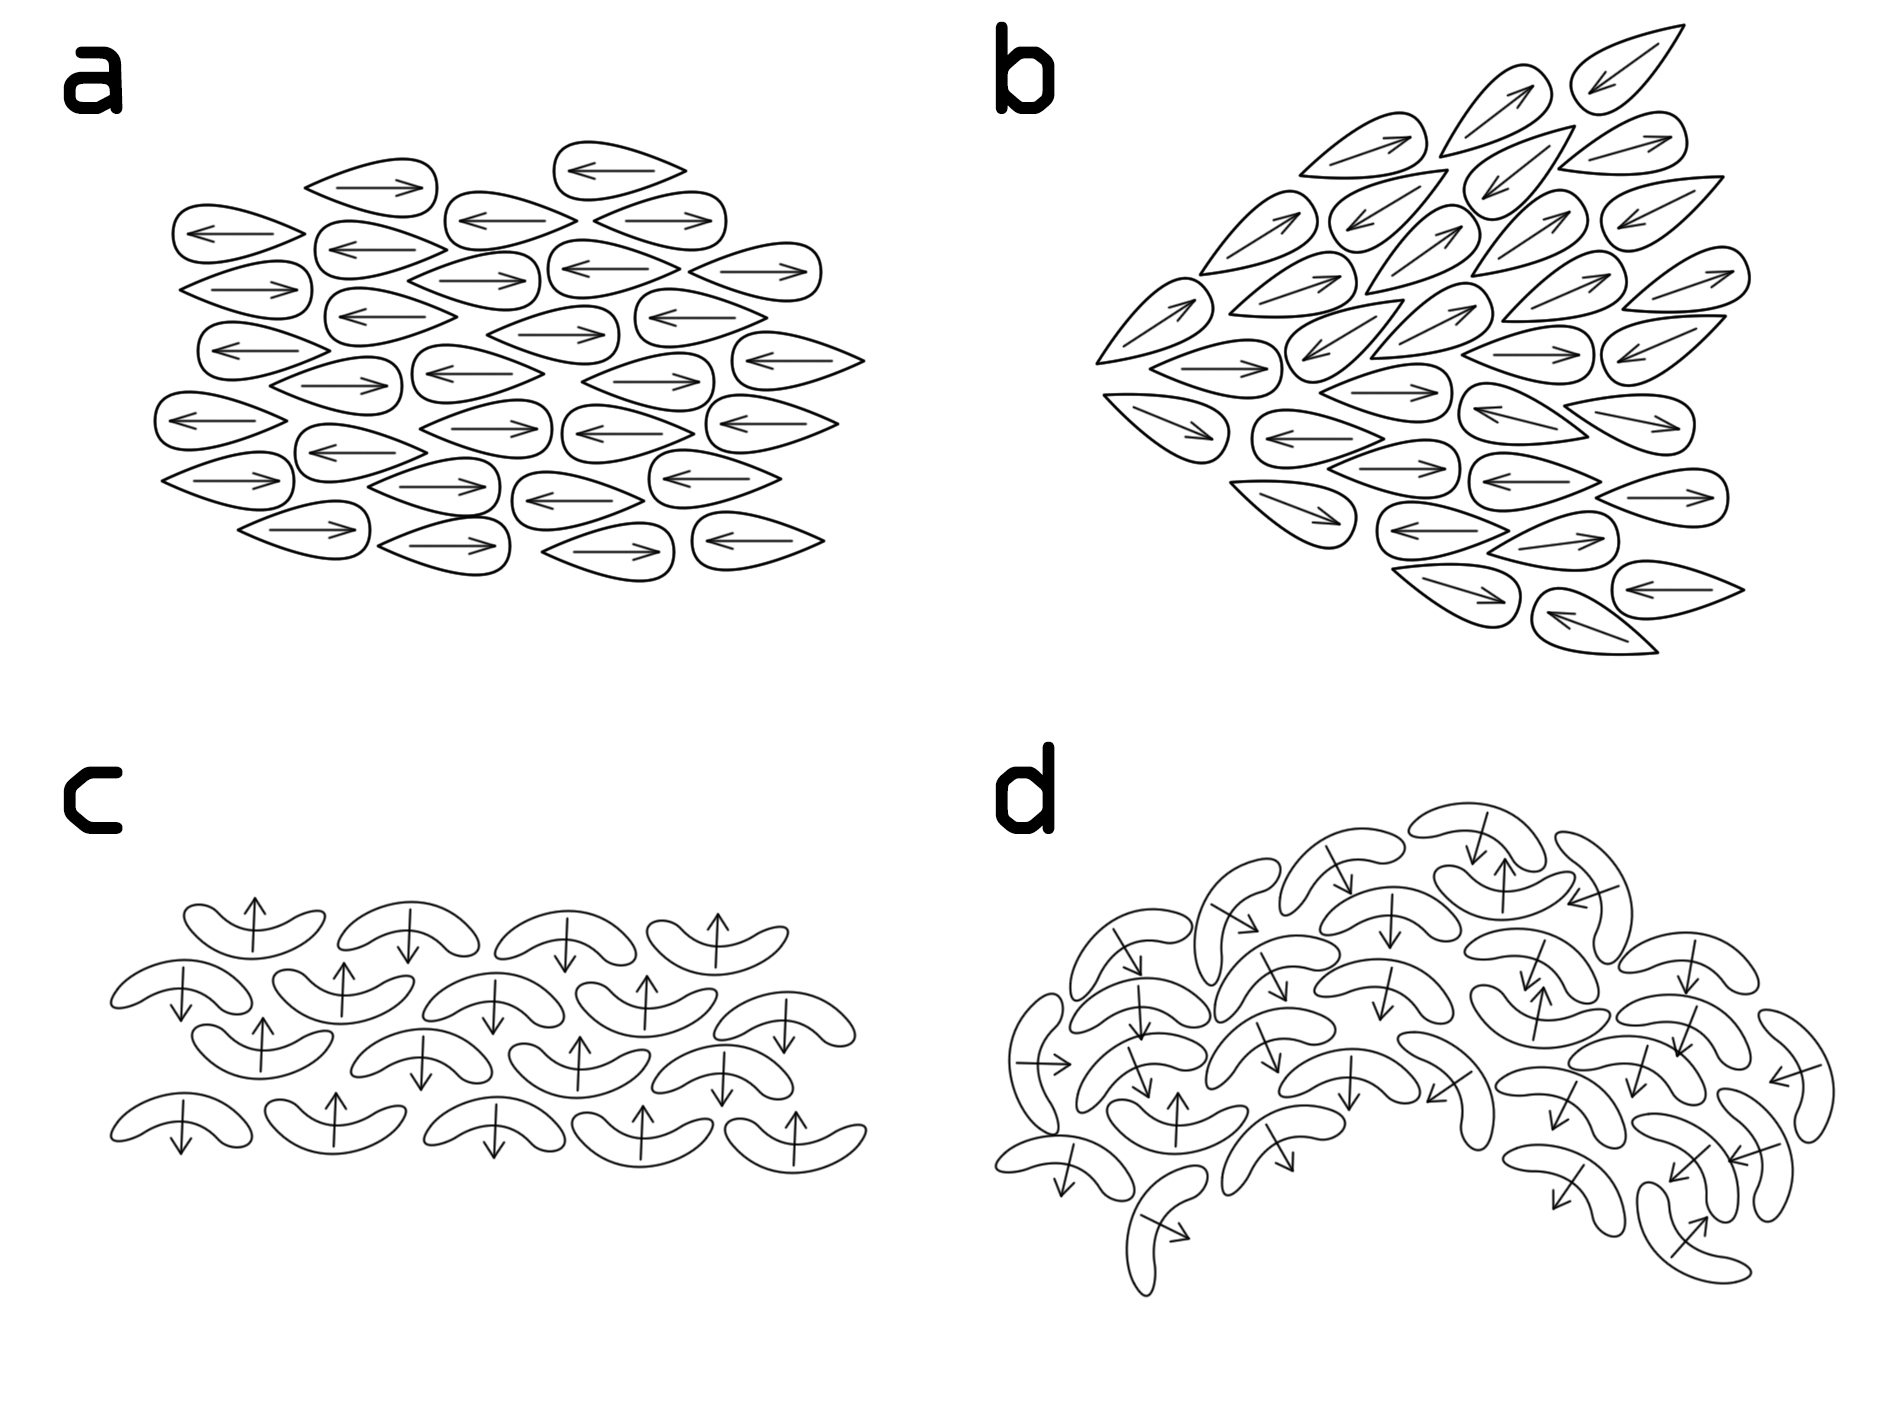
\includegraphics[width=9cm]{Molecules}
%\end{figure}
%\FloatBarrier
%\only<2>{
%\begin{block}{ }
%\begin{equation}
%\FF_\mathrm{e} = \frac{S_\perp}{2} \int\limits_{0}^{L}\left[ K_{11} (\diver{\bb{n}})^2 + K_{22} (\bb{n}\rot{\bb{n}} + q_0)^2 + K_{33} (\bb{n}\times \rot{\bb{n}})^2 \right]\, dz
%\label{F_e from n}
%\end{equation}
%\end{block}
%}
\end{frame}



%\begin{frame}[t]
%\frametitle{Свободная энергия ХЖК во внешнем поле}
%\framesubtitle{Упругая энергия Франка}
%
%
%\begin{block}<1>{ }
%\begin{equation}
%\FF_\mathrm{e} =\frac{V}{2}K_{22}q_0^2 + \frac{S_\perp}{2} \int\limits_{0}^{L}\left[ \AA(\theta) (\theta')^2 + \BB(\theta) (\phi ' )^2 - \CC(\theta)\phi' \right]\, dz
%\label{eq:F_e_basic}
%\end{equation}
%\end{block}
%
%\begin{block}<1>{Введены функции:}
%\begin{align*}
%\AA (\theta) &= K_{11}(\sin{\theta})^2 + K_{33}(\cos{\theta})^2 \\
%\BB (\theta) &= (\sin{\theta})^2 \left( K_{22}(\sin{\theta})^2 + K_{33} (\cos{\theta})^2  \right) \\
%\CC (\theta) &= q_0 K_{22} (\sin{\theta})^2 \\
%\end{align*}
%\end{block}
%\end{frame}


%
%\begin{frame}
%\frametitle{Свободная энергия ХЖК во внешнем поле}
%\framesubtitle{Энергия сцепления с подложкой}
%\begin{block}<1->{ }
%$$
%\FF_\mathrm{sf} = \frac{S_\bot}{2}\sum\limits_{\alpha=1,2} w_\alpha \left( \bb{n}(l_\alpha),\, \bb{n}^{0(\alpha)} \right), \quad l_1 = 0, \quad l_2 = L
%$$
%\end{block}
%
%\begin{block}<1->{Аппроксимация функции $w_\alpha$}
%$$
%w_\alpha \left( \bb{n}(l_\alpha),\, \bb{n}^{0(\alpha)} \right) = w_\alpha (\theta, \phi) = W_\theta^{(\alpha)} \left( \theta - \theta_0^{(\alpha)} \right)^2 + W_\phi^{(\alpha)} \left( \phi - \phi_0^{(\alpha)} \right)^2
%$$
%\end{block}
%\end{frame}

%\begin{frame}[t]
%\frametitle{Свободная энергия ХЖК во внешнем поле}
%\framesubtitle{Вклад внешнего электрического поля}
%
%\begin{block}{ }
%\begin{equation}
%\FF_\mathrm{f} = -\frac{S_\perp}{2} \int\limits_0^L \frac{(\bb{D},\, \bb{E})}{4\pi}\, dz,\quad \epsilon_{ij} = \epsilon_\bot\delta_{ij} + \epsilon_a n_i n_j
%\label{F_f very basic}
%\end{equation}
%\end{block}
%\begin{block}{ }
%\begin{equation}
%\FF_\mathrm{f} = -\frac{S_\bot}{8\pi} U^2 \alert{J}
%\end{equation}
%\end{block}
%\end{frame}





\begin{frame}[t]
\frametitle{Свободная энергия ХЖК во внешнем поле}
\framesubtitle{Полная энергия, записанная в сферических координатах}
\vspace{-0.5cm}
\begin{block}{ }\small
\begin{multline}
\FF_\mathrm{tot} =\frac{V}{2}K_{22}q_0^2 + \frac{S_\perp}{2} \int_{0}^{L}\left[ \AA(\theta) (\theta')^2 + \BB(\theta) (\phi ' )^2- 2\CC(\theta)\phi' \right]\, dz\,+\\
+\frac{S_\perp}{2}\sum\limits_{\alpha=1,2} \left[W_\theta^{(\alpha)} \sin^2{\left( \theta - \theta_0^{(\alpha)} \right)} + W_\phi^{(\alpha)} \sin^2{\left( \phi - \phi_0^{(\alpha)} \right)}\right] -\\
-\frac{S_{\!\bot}}{8\pi}U^2 J +S_{\!\bot} \bar{e}_{13}U JJ_1+2\pi S_{\!\bot} \bar{e}_{13}^2\left(\int_{0}^{L}\frac{(\sin 2\theta \,\theta')^2}{{\EE}(\theta)}dz -JJ_1^2\right)
%\label{eq:free-energy}
\end{multline}
\begin{align*}
\AA (\theta) &= K_{11}(\sin{\theta})^2 + K_{33}(\cos{\theta})^2 \\
\BB (\theta) &= (\sin{\theta})^2 \left( K_{22}(\sin{\theta})^2 + K_{33} (\cos{\theta})^2  \right) \\
\CC (\theta) &= q_0 K_{22} (\sin{\theta})^2 \\
\end{align*}

\end{block}
\end{frame}

\begin{frame}
	\frametitle{Свободная энергия ХЖК во внешнем поле}
	\framesubtitle{Упрощение функционала свободной энергии}
	%\begin{block}{Уравнения Эйлера-Лагранжа}
		После варьирования $\FF_\mathrm{tot}$ получаем систему уравнений Эйлера-Лагранжа
		\begin{eqnarray}
			&&\frac{d\AA}{d\theta}\theta'^2 + 2\AA \theta'' = \frac{d B}{d\theta}\phi'^2 - 2\frac{d C}{d\theta}\phi'
			+ \frac{\varepsilon_a\EuScript{U}^2\! J ^2\!\sin 2\theta}{4\pi\EE^2(\theta)} ,
			\label{eq:E-L1}\\
			&&{d}\left( B\phi' - C \right)/{dz} = 0,
			\label{eq:E-L2}
		\end{eqnarray}
		и систему граничных условий ($\alpha =1,2$)
		\begin{eqnarray}
			&&\left(2(-1)^\alpha [{\AA(\theta)\theta'} + \bar{e} {\EuScript{U}}J\sin2\theta/\EE(\theta)]\phantom{ W_\phi^{(\alpha)}}\right. + \nonumber\\
			&&\hspace{27mm}\left.\left.+ W_\theta^{(\alpha)}\sin2(\theta - \theta_0^{(\alpha)})\right) \right|_{z=l_\alpha} = 0,\label{eq:gran-1}\\
			&&{\left.\left(2(-1)^\alpha (B\phi' - C)
			+W_\phi^{(\alpha)}\sin2(\phi - \phi_0^{(\alpha)})\right) \right|_{z=l_\alpha}} = 0,
			\label{eq:gran-2}
		\end{eqnarray}
	%\end{block}
\end{frame}

\begin{frame}
	\frametitle{Свободная энергия ХЖК во внешнем поле}
	\framesubtitle{Упрощение функционала свободной энергии}
	Окончательные выражение для $\FF_\mathrm{tot}$
	\begin{multline}
		\FF_\mathrm{tot}(\theta) = \FF^{(0)}_e + \frac{S_{\!\bot}}{2}\Bigg[\int_0^L \left({ \AA(\theta)}\theta'^2 - \frac{C^2(\theta)}{B(\theta)} \right) dz +\\
		+W_\theta^{(1)}\sin^2 \left( \theta(0) - \theta_0^{(1)} \right)+W_\theta^{(2)}\sin^2 \left( \theta(L) - \theta_0^{(2)} \right) +\\
		+ C_2^2\left(I_1+{\kappa_1}/{W^{(1)}_\varphi}+{\kappa_2}/{W^{(2)}_\varphi}\right)-{\frac{\EuScript{U}^2 J}{4\pi} }\Bigg],
		\label{eq:F_for_minimization}
	\end{multline}
	и $\phi$:
	\begin{equation}\label{eq:phi_profile}
		\varphi(z)=\varphi_0^{(1)}+\frac12\arcsin\frac{2C_2}{W^{(1)}_\varphi}
		+ \int_0^z \frac{C(\theta)+C_2}{B(\theta)}\, dz .
	\end{equation}
\end{frame}

\begin{frame}
	\frametitle{Свободная энергия ХЖК во внешнем поле}
	\framesubtitle{Выражения для констант}
	В формулах~\eqref{eq:F_for_minimization} и~\eqref{eq:phi_profile} используются константы $C_2$ и $\kappa_{1,2}$. Для $\kappa_{1,2}$ можно привести точное выражение:
	\begin{equation}
		\kappa_\alpha=2/\Big(1+\sqrt{1-\big(2C_2/W^{(\alpha)}_\varphi\big)^2}\Big),
	\end{equation}
	а на $C_2$ имеется трансцендентное уравнение:
	\begin{equation}\label{eq:C2iteration}
		C_2=(\varphi_\mathrm{tot}^{(0)}-I_2)/\big(I_1+k_1/W^{(1)}_\varphi + k_2/W^{(2)}_\varphi \big),
	\end{equation}
	где $k_\alpha=\left(W^{(\alpha)}_\varphi/2C_2\right)\arcsin\left(2C_2/W^{(\alpha)}_\varphi \right)$, $1\leq k_\alpha\leq \pi/2$.
\end{frame}


%
%\begin{frame}
%\frametitle{Уравнения Эйлера-Лагранжа}
%\begin{block}<1->{ }
%\begin{equation}
%\frac{d\AA}{d\theta}\,\theta'^2 + 2\AA \theta'' = \frac{d\BB}{d\theta}\,\phi'^2 - 2\frac{d\CC}{d\theta}\,\phi'
 %+ \left( -\frac{U^2}{4\pi} + \frac{2\overline{e}_{13}}{\epsilon_a}J_1 U\right)\frac{d\EE}{d\theta}\, \EE^{-2} J ^2,
%\label{eq:E-L1}
%\end{equation}
%\begin{equation}
%\frac{d}{dz}\left( \BB\phi' - \CC \right) = 0.
%\label{eq:E-L2}
%\end{equation}
%\end{block}
%
%\begin{block}<2>{ }
%\begin{equation}
%\left(\left.2(-1)^\alpha [\AA(\theta) \theta' - \overline{e}_{13} UJ\sin2\theta/\EE(\theta) ]+ W_\theta^{(\alpha)}(\theta - \theta_0^{(\alpha)})\right) \right|_{z=l_\alpha} = 0,
%\label{eq:gran-1}
%\end{equation}
%\begin{equation}
%\left(\left.2(-1)^\alpha (\BB\phi' - \CC) + W_\phi^{(\alpha)}(\phi - \phi_0^{(\alpha)})\right) \right|_{z=l_\alpha} = 0,\quad \alpha = 1,\, 2.
%\label{eq:gran-2}
%\end{equation}
%\end{block}
%\end{frame}









%
%
%\begin{frame}
%\frametitle{Численная минимизация $\FF_\mathrm{tot}$}
%\begin{figure}
%\centering
%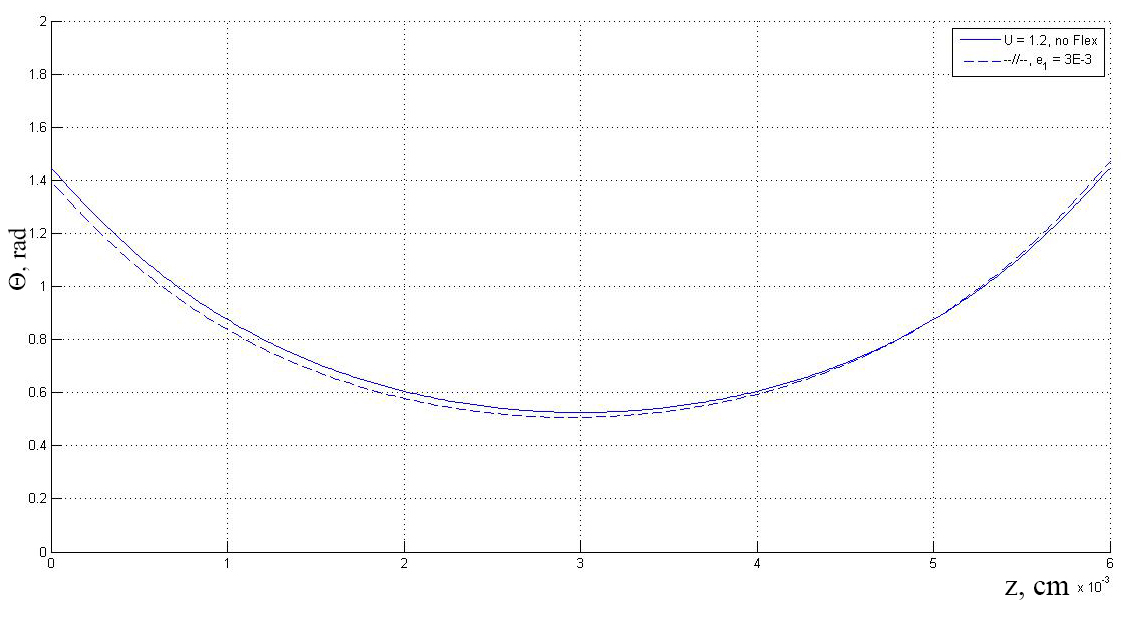
\includegraphics[width=0.95\textwidth]{pic3}
%\caption{Сравнение равновесных конфигураций $\theta(z)$ при $U = 1.2\, V$, найденных с учётом и без учёта флексоэлектрической поляризации}
%\end{figure}
%\FloatBarrier
%\end{frame}
%
%\begin{frame}
%\frametitle{Результаты уточнённого численного счёта}
%\begin{figure}[ht]
%\centering
%\begin{minipage}{0.49\textwidth}
%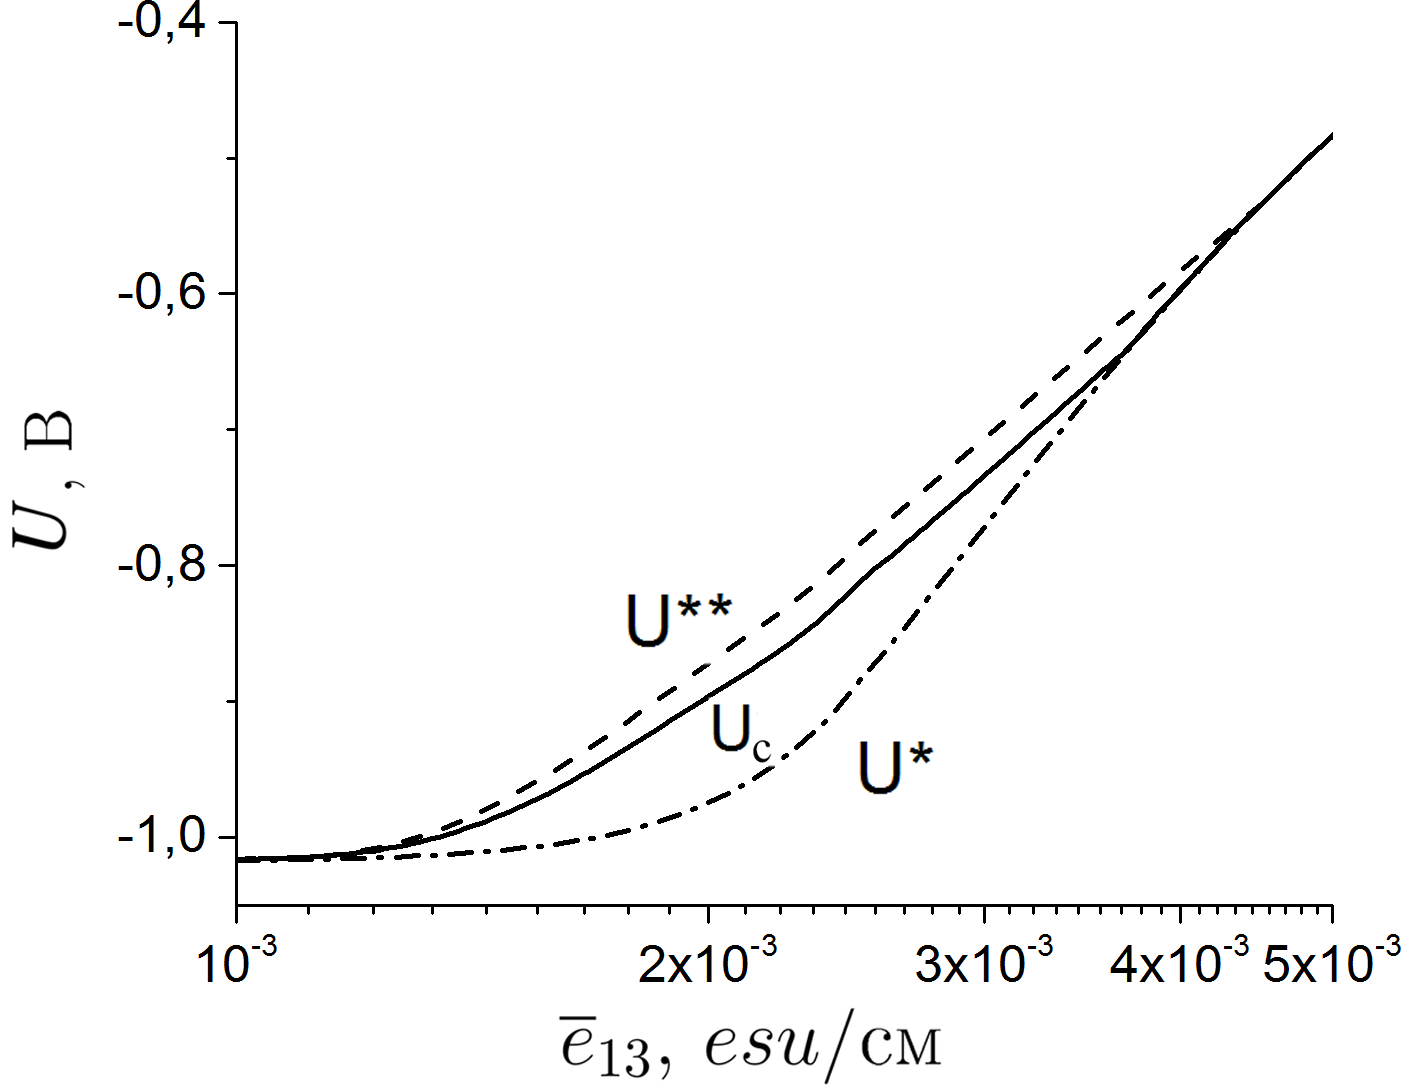
\includegraphics[width=\textwidth]{Graph2}
%%\caption{}
%\caption{\vspace{-1cm}1 -- $U_{**}$, 2 -- $U_c$, 3 -- $U_*$}
%\label{pic-Profiles_for_different_N}
%\end{minipage}
%\hfil
%\begin{minipage}{0.49\textwidth}
%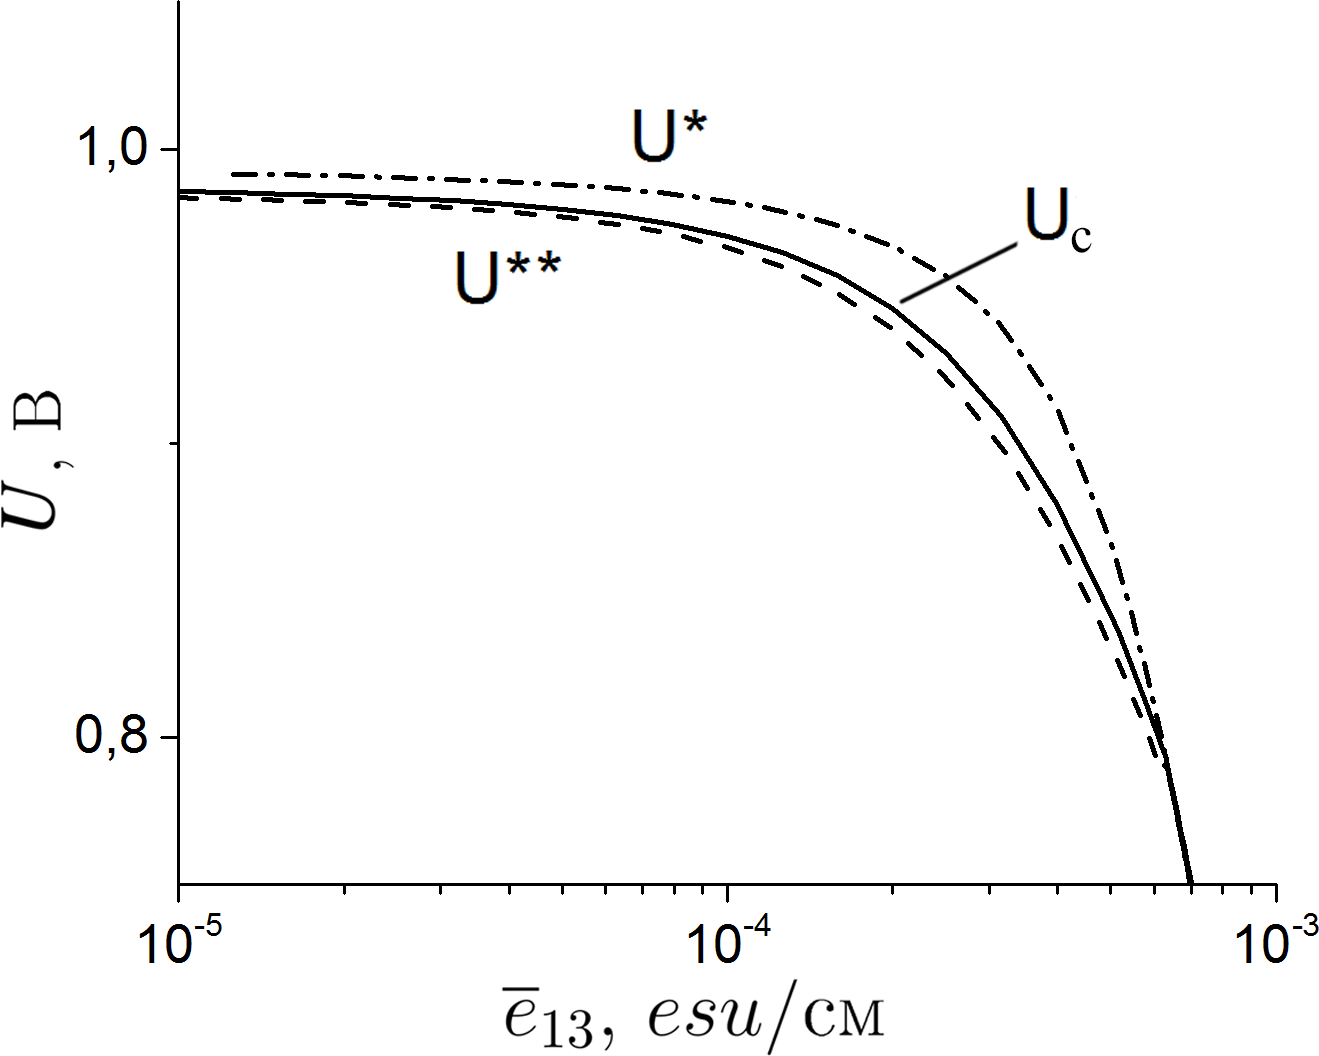
\includegraphics[width=\textwidth]{Graph3}
%\caption{\vspace{-1cm}1 -- $U_{**}$, 2 -- $U_c$, 3 -- $U_*$}
%\label{pic-Profiles_for_different_N}
%\end{minipage}
%\end{figure}
%\FloatBarrier
%\end{frame}

\begin{frame}
	\centering
	{\large Часть 2. Влияние флексоэлектричества на переход Фредерикса (случай отрицательной диэлектрической анизотропии)\blfootnote{Результаты опубликованы в статье \textit{A.~D.~Oskirko, S.~V.~Ul'yanov and A.~Yu.~Val'kov} \textbf{Effect of flexoelectricity on the Frèedericksz transition in chiral nematics with negative dielectric anisotropy} J. Phys.: Conf. Ser. 1141 012147}}%, DOI:~10.1103/PhysRevE.98.012702}}
\end{frame}

\begin{frame}
\frametitle{Устойчивость планарной геликоидальной структуры}
\framesubtitle{Аналитическое изучение}\vspace{-0.2cm}
\begin{block}<1->{ }
\begin{equation}
\delta^2\FF_\mathrm{tot} = \delta^2\FF_\theta + \delta^2\FF_\phi,\notag
\end{equation}
\end{block}
\begin{block}{ }
\begin{align}
\delta^2 \FF_\theta &=
\frac{S_\bot}{2}\int_{0}^{L}\left(K_{11}(\delta\theta')^2 + M(\delta\theta)^2\right)\, dz+\\
&+\frac{S_\bot}{2}\sum_{\alpha=1,2}\alert{\EuScript{W}_\theta^{(\alpha)}}\delta\theta^2(l_\alpha),\notag
\end{align}
\begin{equation}
\delta^2 \FF_\phi =
\frac{S_\bot}{2}\int_{0}^{L}\left(K_{22}(\delta \phi')^2\right)\, dz+\frac{S_\bot}{2}\sum_{\alpha=1,2}W_\phi^{(\alpha)}\delta\phi^2(l_\alpha),
\end{equation}
\end{block}
\begin{block}{ }
\begin{equation}\label{W_tilde}
\begin{aligned}
&M = K_{33}q_0^2 - \epsilon_a U^2/(4\pi L^2) > 0,\\
&\EuScript{W}_\theta^{(\alpha)} = W_\theta^{(\alpha)} - 2(-1)^\alpha \overline{e}_{13} U/L
\end{aligned}
\end{equation}
\end{block}
\end{frame}

%\begin{frame}
%\frametitle{Устойчивость планарной геликоидальной структуры}
%\framesubtitle{Случаи нарушения устойчивости}
%\begin{block}{ }
%\begin{table}[ht!]
%\centering
%\begin{tabular}{cccc}
%$I$ & : & $M < 0$, & $\widetilde{W}_\theta^{-} > 0$,\\
%$II$ & : & $M > 0$, & $\widetilde{W}_\theta^{-} < 0$,\\
%$III$ & : & $M < 0$, & $\widetilde{W}_\theta^{-} < 0$.\\
%\end{tabular}
%\end{table}
%\FloatBarrier
%\end{block}
%\begin{block}{ }
%\begin{table}[ht!]
%\centering
%\begin{tabular}{cccc}
%$I$ & : & $\abs{U} >  q_0 L \sqrt{4\pi K_{33}/\varepsilon_a} \equiv U_\mathrm{Fr}$, & $\abs{U} < \frac{W_\theta^- L}{2\overline{e}_{13}} \equiv U_\mathrm{Fl}$,\\
%$II$ & : & $\abs{U} < U_\mathrm{Fr}$, & $\abs{U} > U_\mathrm{Fl}$,\\
%$III$ & : & $\abs{U} > U_\mathrm{Fr}$, & $\abs{U} > U_\mathrm{Fl}.$
%\end{tabular}
%\end{table}
%\FloatBarrier
%\end{block}
%\end{frame}














\begin{frame}
\frametitle{Устойчивость планарной геликоидальной структуры}
%\begin{block}{ }
%\begin{align}
%\delta^2 \FF_\theta &=
%\frac{S_\bot}{2}\int_{0}^{L}\left(K_{11}(\delta\theta')^2 + M(\delta\theta)^2\right)\, dz+\frac{S_\bot}{2}\sum_{\alpha=1,2}\widetilde{W}_\theta^{(\alpha)}\delta\theta^2(l_\alpha),\notag
%\end{align}
%\end{block}

\begin{block}{ }
$$
\delta\theta(z) = \delta\psi(z) + \delta\mu(z),\quad\delta^2 \FF_\theta = Q_\psi + Q_\mu,
$$
\begin{equation}\label{Qdelta0}
Q_\psi= \frac{S_\bot}{2}\int_{0}^{L}\left(K_{11}(\delta\psi'(z))^2+M(\delta\psi(z))^2\right)\mathrm{d}z + \frac{S_\bot}{2}\sum_{\alpha=1,2}\widetilde{W}_\theta^{(\alpha)}\delta_\alpha^2,
\end{equation}
\begin{equation}\label{Qmu}
Q_\mu=\frac{S_\bot}{2}\int_{0}^{L}\left(K_{11}(\delta\mu')^2+M(\delta\mu)^2\right)\mathrm{d}z.
\end{equation}
\end{block}


\begin{block}{ }
%\begin{equation}\label{thetamupsi}
%\delta\theta(z) = \delta\psi(z) + \delta\mu(z),
%\end{equation}
$$
K_{11} \delta\psi''(z) - M\delta\psi(z) = 0,\quad \delta\psi(0) = \delta_1,\quad \delta\psi(L) = \delta_2.
$$
\begin{equation}\label{psi=}
\delta\psi =
\displaystyle\delta_1\frac{\sinh \xi(L-z)}{\sinh\xi L}+\delta_2\frac{\sinh\xi z}{\sinh\xi L},
\end{equation}
$$\xi = \sqrt{M/K_{11}}.$$
\end{block}
\end{frame}


%\begin{frame}
%\frametitle{Устойчивость планарной геликоидальной структуры}
%\begin{block}{ }
%$$
%\delta\theta(z) = \delta\psi(z) + \delta\mu(z),\quad\delta^2 \FF_\theta = Q_\psi + Q_\mu,
%$$
%\begin{equation}\label{Qdelta0}
%Q_\psi= \frac{S_\bot}{2}\int_{0}^{L}\left(K_{11}(\delta\psi'(z))^2+M(\delta\psi(z))^2\right)\mathrm{d}z + \frac{S_\bot}{2}\sum_{\alpha=1,2}\widetilde{W}_\theta^{(\alpha)}\delta_\alpha^2,
%\end{equation}
%\begin{equation}\label{Qmu}
%Q_\mu=\frac{S_\bot}{2}\int_{0}^{L}\left(K_{11}(\delta\mu')^2+M(\delta\mu)^2\right)\mathrm{d}z.
%\end{equation}
%\end{block}
%\end{frame}

%\begin{frame}
%\frametitle{Устойчивость планарной геликоидальной структуры}
%\framesubtitle{Анализ знака форм $Q_\mu$ и $Q_\psi$}
%\only<1->{
%\begin{block}{Условие положительной определённости $Q_\mu$}
%\begin{equation}\label{xiL<pi}
%\xi L < \pi.
%\end{equation}
%\end{block}
%}
%\only<1->{
%\begin{block}{$Q_\psi$ на планарной геликоидальной структуре}
%\begin{equation*}\hspace{-0cm}
%Q_\psi=
%\begin{cases}
%\frac{S_\bot}{2}\sum\limits_{\alpha=1,2}\left(K_{11}\xi \ctg{\xi L}+\widetilde{W}_\theta^{(\alpha)}\right) \delta_\alpha^2 - S_\bot K_{11}(\xi/\sin\xi L)\delta_1\delta_2, M<0.\\
%\frac{S_\bot}{2}\sum\limits_{\alpha=1,2}\left(K_{11}\zeta \cth{\zeta L}+\widetilde{W}_\theta^{(\alpha)}\right) \delta_\alpha^2 - S_\bot K_{11}(\zeta/\sh\zeta L)\delta_1\delta_2, M>0.\\
%\end{cases}
%\end{equation*}
%\end{block}
%}
%\only<2->{
%\begin{block}{Условия положительной определённости $Q_\psi$ при M < 0}
%\begin{equation*}\label{SC2-1}
%\begin{cases}
%\widetilde{W}_\theta^{(1)}+K_{11}\xi\ctg\xi L>0,\\
%\widetilde{W}_\theta^{(1)}\widetilde{W}_\theta^{(2)}+K_{11}(\widetilde{W}_\theta^{(1)}+\widetilde{W}_\theta^{(2)}) \xi\ctg\xi L>\xi^2K_{11}^2
%\end{cases}
%\end{equation*}
%\end{block}
%}
%\only<2->{
%\begin{block}{Условия положительной определённости $Q_\psi$ при M > 0}
%\begin{equation*}\label{SC2-2}
%\begin{cases}
%\widetilde{W}_\theta^{(1)}+K_{11}\zeta\cth\zeta L>0,\\
%\widetilde{W}_\theta^{(1)}\widetilde{W}_\theta^{(2)}+K_{11}(\widetilde{W}_\theta^{(1)}+\widetilde{W}_\theta^{(2)}) \zeta\cth\zeta L>-\zeta^2K_{11}^2
%\end{cases}
%\end{equation*}
%\end{block}
%}
%\end{frame}

\begin{frame}
\frametitle{Устойчивость планарной геликоидальной структуры}
\begin{block}{Результирующий критерий устойчивости:}
\begin{equation}\label{stab_cond_final}
w^{(1)}w^{(2)}+2\bar{w}   t \coth t+ t^2>0.
\end{equation}
\end{block}
где введены безразмерные параметры $t = \xi L$,  $w^{(\alpha)}={\EuScript{W}^{(\alpha)} L}/{K_{11}}$, и $\bar{w}=({W}^{(1)}_\theta+{W}^{(2)}_\theta)L/2K_{11}$.
\begin{block}{Уравнение кривой $e^*_+(U)$}
	\begin{equation}\label{eq:!!}
		e_{+}^*(U)=\left(K_{11}/4U\right)\left(\Delta{w}+ 2\bar{w}\sgn{U}\sqrt{ 1+X(U) }\right) ,
	\end{equation}
	\begin{equation}\label{eq:e(U)_ea<0}
		X(U)=\frac{2}{\bar{w}} \left( t\coth t +{t^2}/2\bar{w} \right).
	\end{equation}
\end{block}
Уравнение вертикальной асимптоты:
\begin{equation}
\bar{e}' = \lim_{U\to \infty} \bar{e}^*_+(U) = \sqrt{\frac{-\varepsilon_a K_{11}}{16\pi}}
\end{equation}
\end{frame}

%\begin{frame}
%\frametitle{Устойчивость планарной геликоидальной структуры}
%\framesubtitle{Теория Ландау}
%\begin{block}{Представление $\theta(z)$}
%\begin{equation}\label{theta_easy}
%\theta(z) = \pi/2 + \delta\psi(z),
%\end{equation}
%\end{block}
%\begin{block}{Разложение $\FF_\mathrm{tot}$}
%\begin{equation}\label{Landau_general}
%\FF_\mathrm{tot} = \FF^{(0)}+ \sum\limits_{k=0}^2A_k(U)\delta_1^k\delta_2^{2-k} + \sum\limits_{k=0}^4 B_k(U)\delta_1^k\delta_2^{4-k}
%\end{equation}
%\end{block}
%\end{frame}


%
%\begin{frame}
%\frametitle{Устойчивость планарной геликоидальной структуры}
%\begin{figure}[ht]
%\centering
%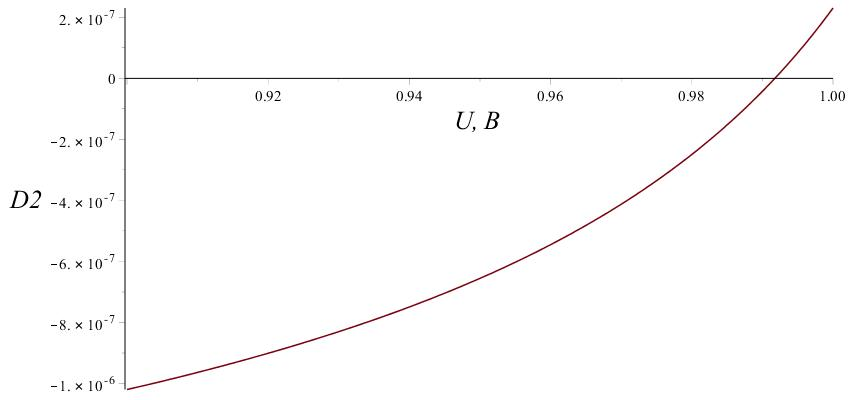
\includegraphics[width=12cm]{Discriminant_example}
%\caption{Пример зависимости дискриминанта квадратичной формы $\FF^{(2)}$ от напряжения $U$.}
%\label{D2_from_U}
%\end{figure}
%\FloatBarrier
%\end{frame}





\begin{frame}
\frametitle{Переход Фредерикса. Случай $\varepsilon_a < 0$}
\framesubtitle{Фазовые диаграммы}
\begin{figure}[h]
\includegraphics[width=0.49\textwidth]{1aa.eps}%{PhD_negative_ea.png}\hspace{2pc}%
\includegraphics[width=0.49\textwidth]{1bb.eps}%{PhD_negative_ea.png}\hspace{2pc}%
\caption{Фазовые диаграммы для случаев $\varepsilon_a < 0$ и $\varepsilon_a > 0$. Сплошная и пунктирная линии соответствуют межфазным границам, соответственно, для непрерывного и для разрывного перехода; линией из точек обозначена асимптота  межфазовой границы при $\varepsilon_a < 0$, а кружок обозначает трикритическую точку.}
\end{figure}
\end{frame}

\begin{frame}
\frametitle{Переход Фредерикса. Случай $\varepsilon_a < 0$}
\framesubtitle{Сравнение профилей $\theta(z)$ при постоянном $U$}
\begin{figure}[h]
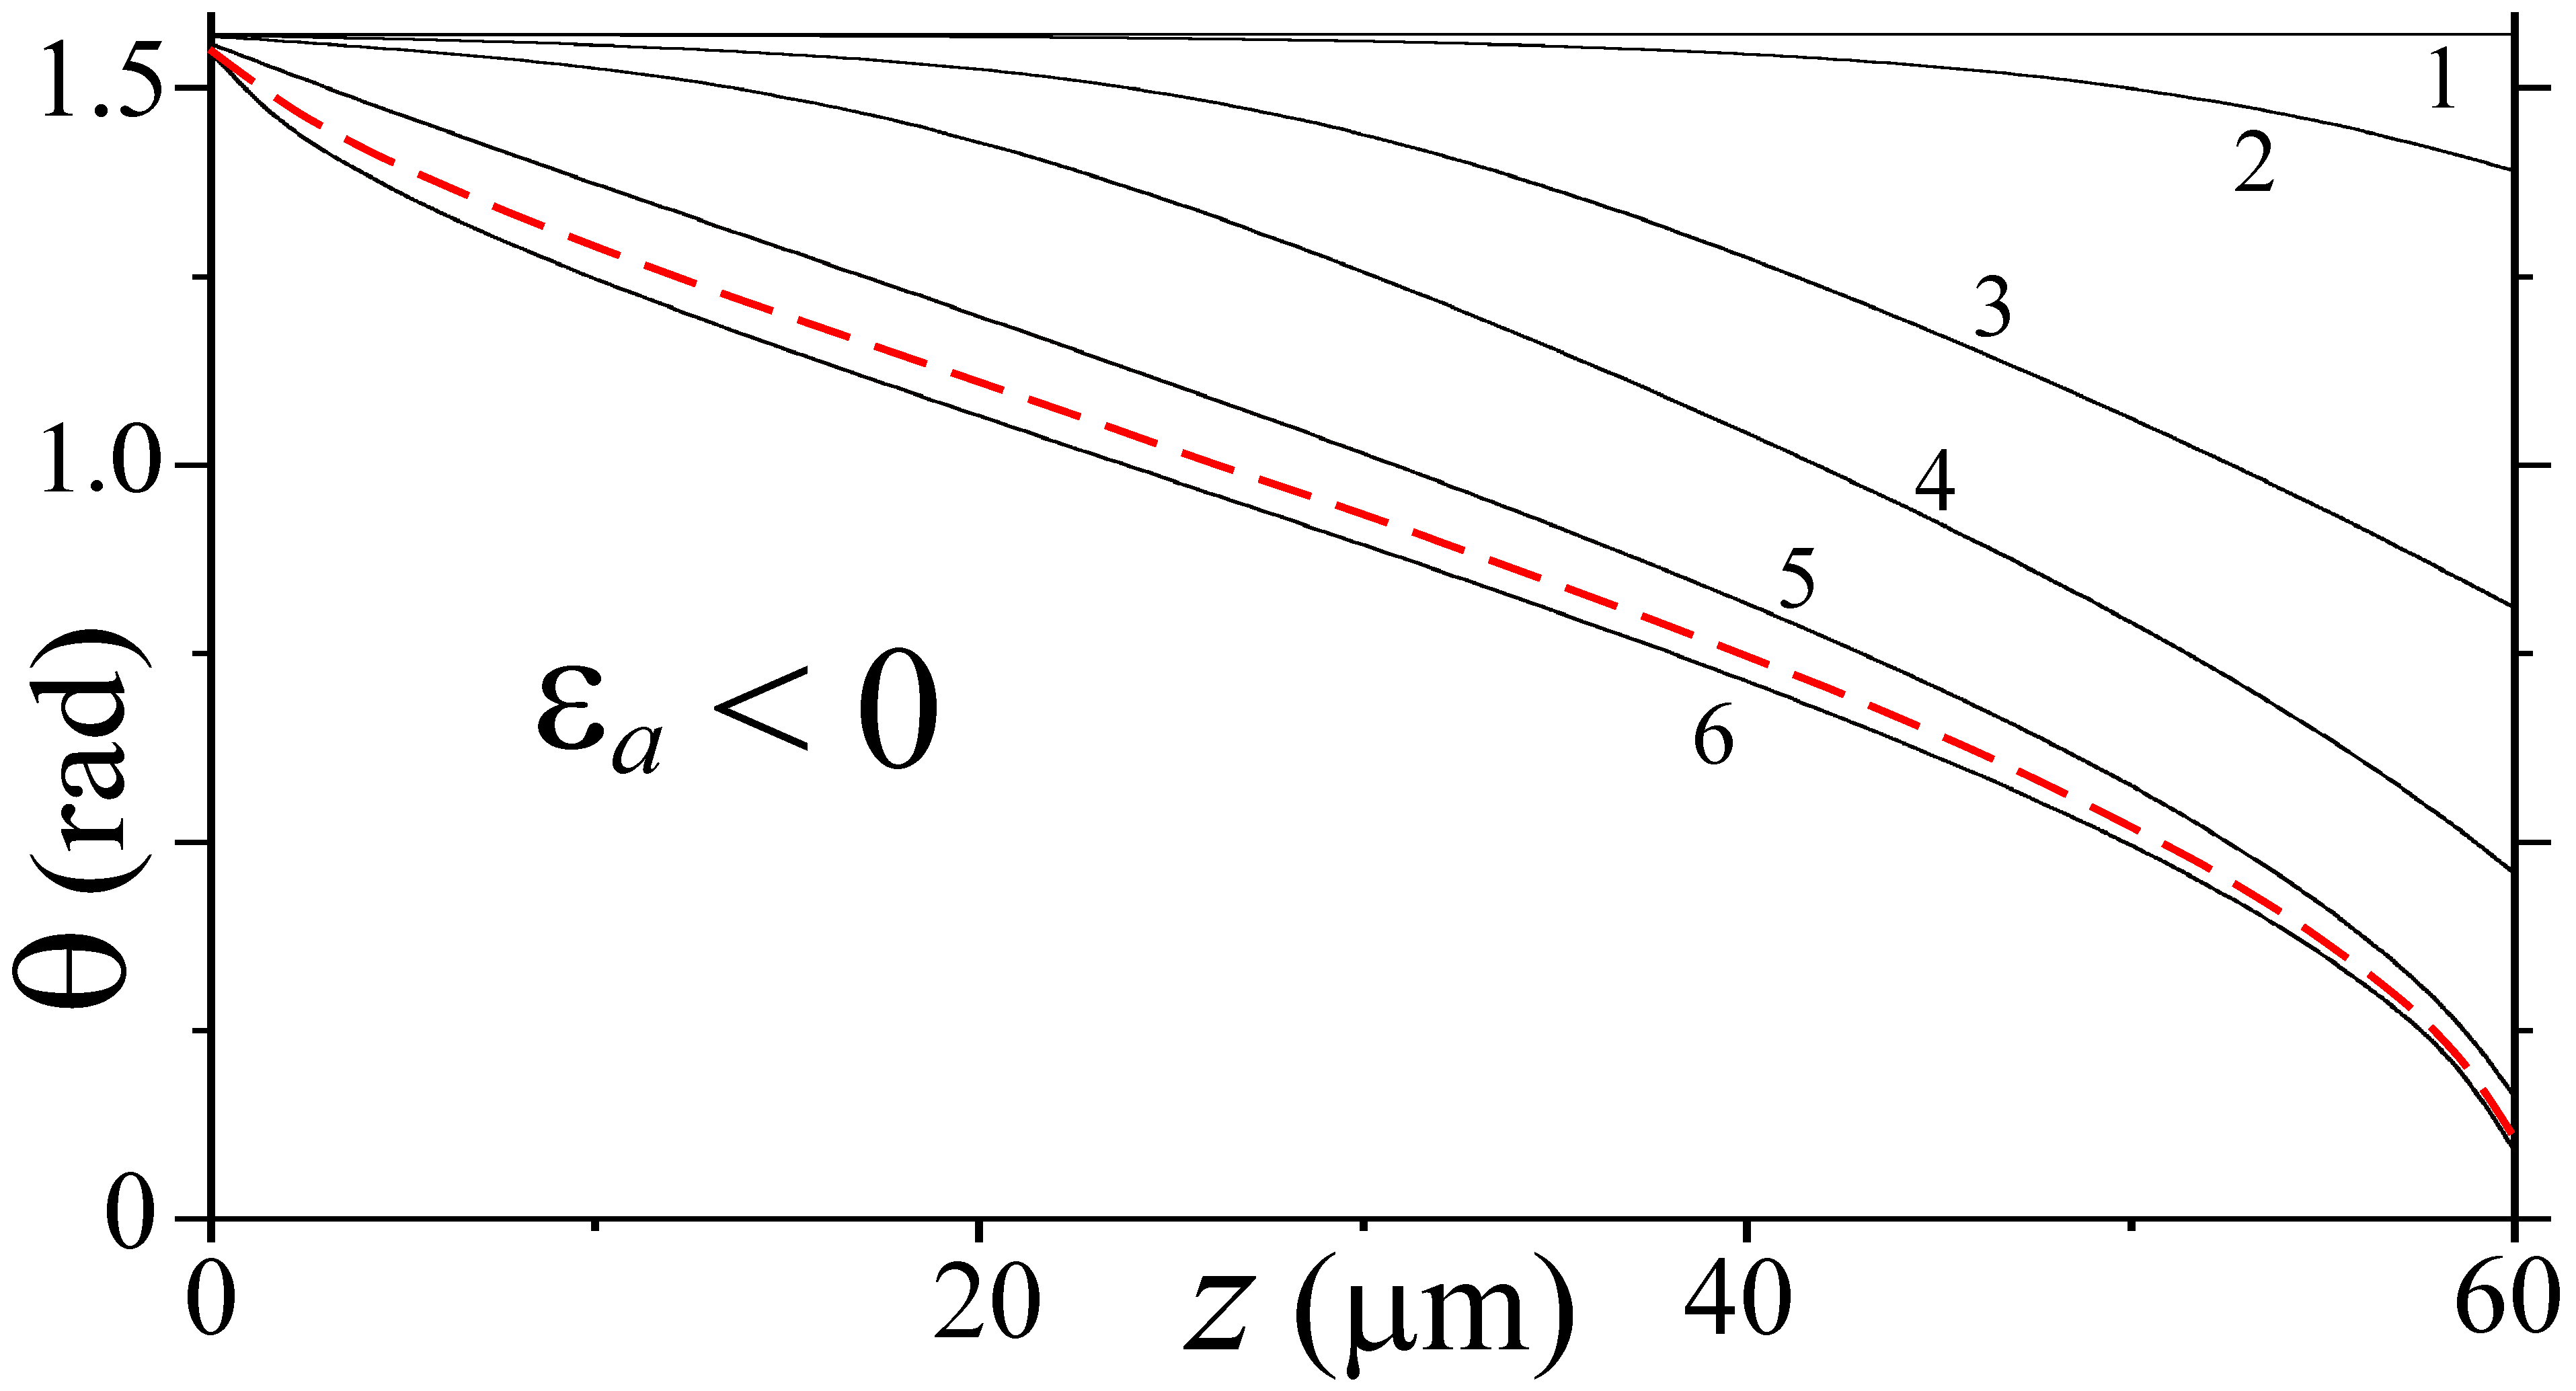
\includegraphics[width=0.49\textwidth]{Fig4_parody1a.eps}%\hspace{2pc}%
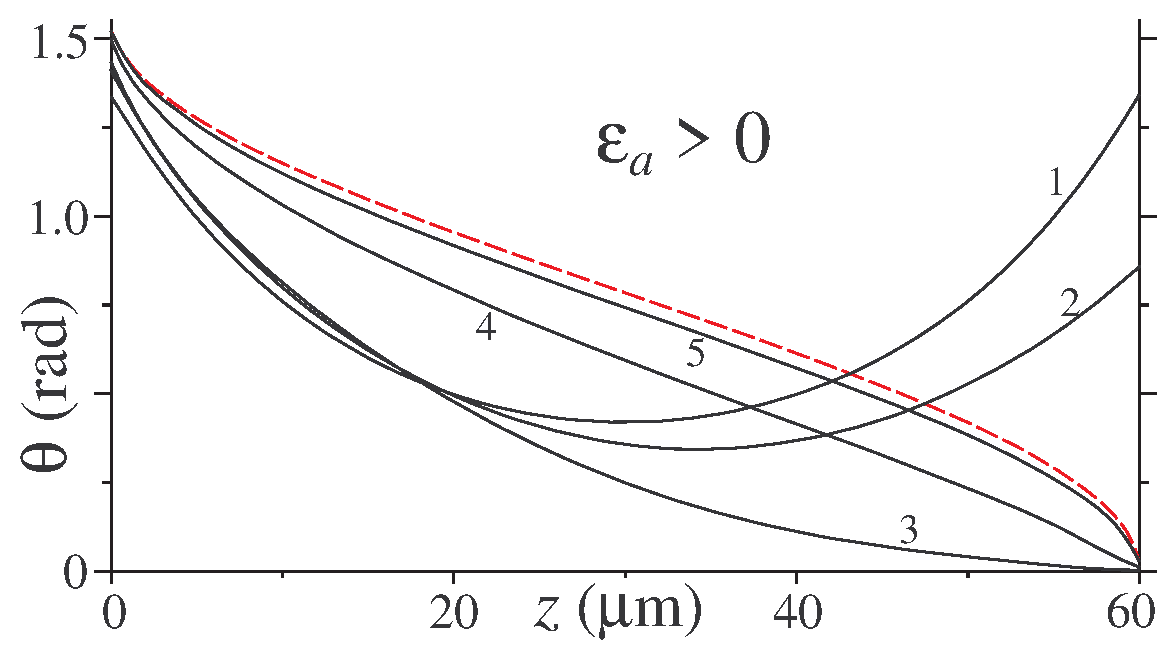
\includegraphics[width=0.49\textwidth]{symm_all_6curvesNoReflect1b.eps}
\caption{ Профили $\theta(z)$ для $U=1.2 ~V$. Линии для $\varepsilon_a<0$ соответствуют: 1 -- $\bar{e}=10^{-3}$, 2 -- $\bar{e}=1.5\times 10^{-3}$, 3 -- $\bar{e}=1.8\times 10^{-3}$, 4 -- $\bar{e}=2\times 10^{-3}$, 5 -- $\bar{e}=3\times 10^{-3}$, 6 -- $\bar{e}=10^{-2}$  в единицах $ \mathrm{statC/cm}$; линии для  $\varepsilon_a > 0$ соответствуют: 1 -- $\bar{e}=0$, 2 -- $\bar{e}=10^{-4}$, 3 -- $\bar{e}=10^{-3}$, 4 -- $\bar{e}=3\times 10^{-3}$, 5 -- $\bar{e}=10^{-2}$ в единицах $\mathrm{statC/cm}$. Пунктирные линии соответствуют зависимости $\cos^2\theta(z)\simeq {z/L}$.}
\end{figure}
\end{frame}

\begin{frame}
\frametitle{Переход Фредерикса. Случай $\varepsilon_a < 0$}
\framesubtitle{Сравнение профилей $\theta(z)$ при постоянном большом $\bar{e}$}
\begin{figure}[h]
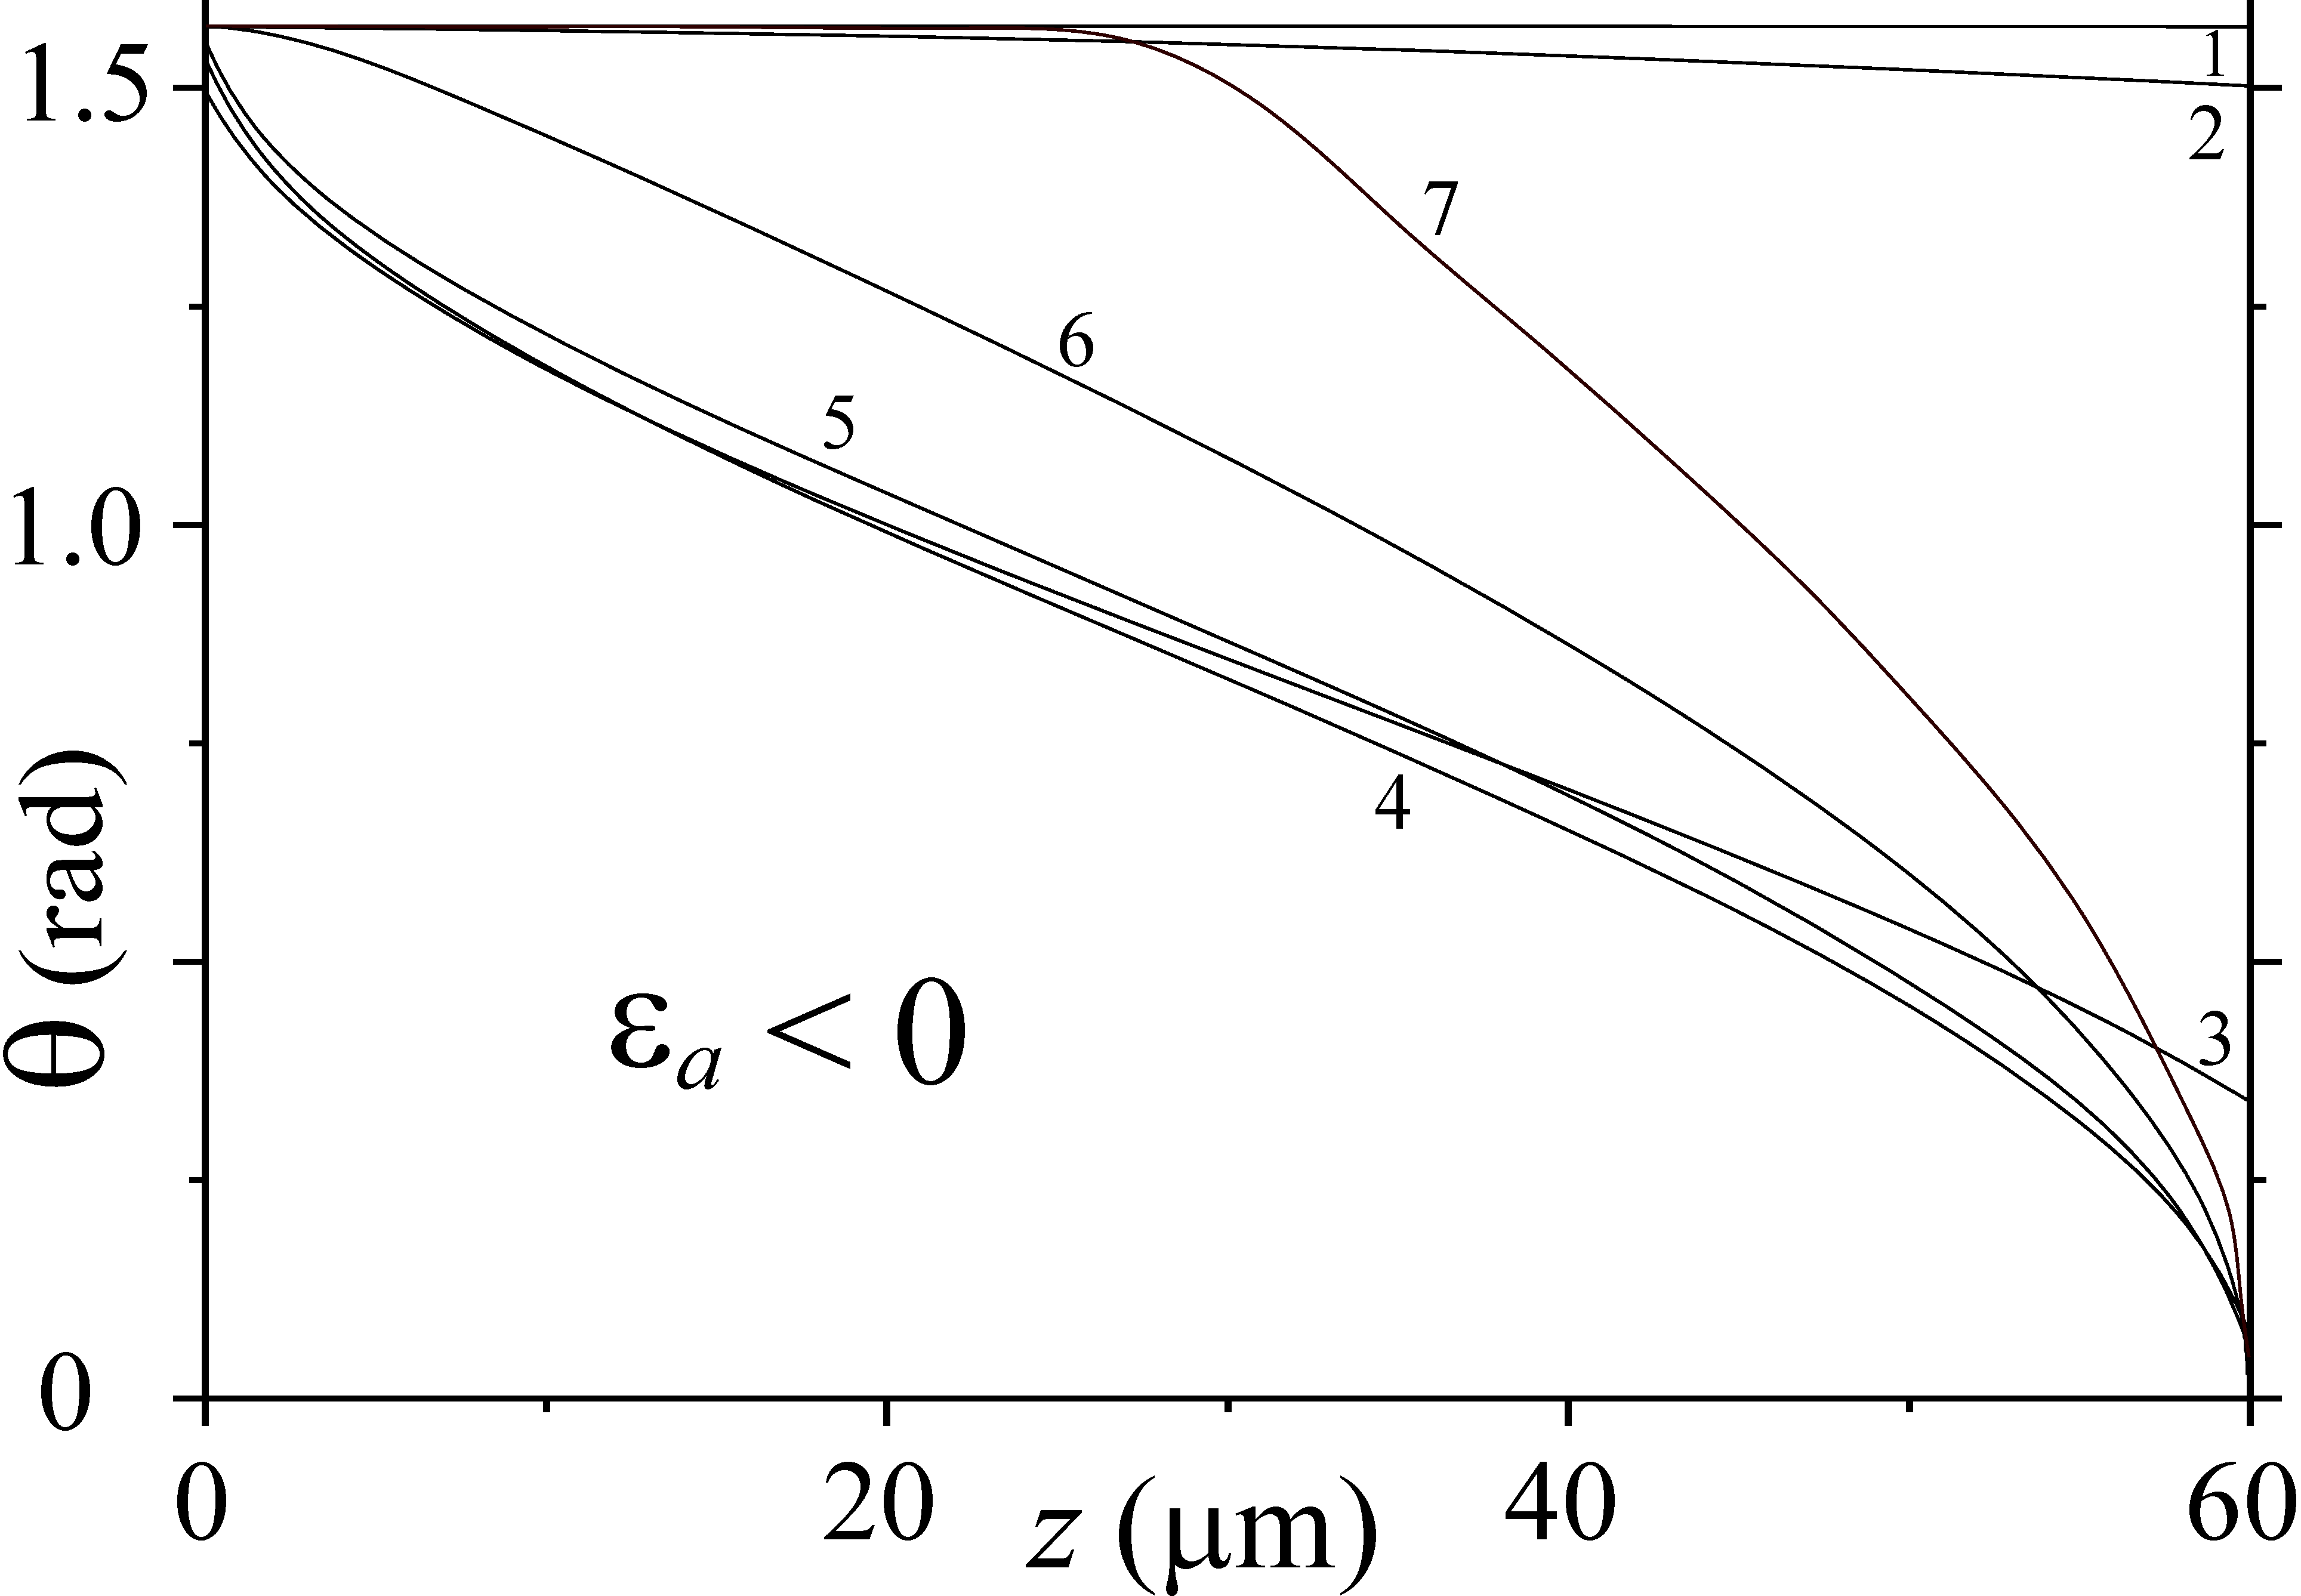
\includegraphics[width=0.49\textwidth]{Profiles_at_fixed_e_0_01_change_U.eps}%\\
%\hspace{5mm}
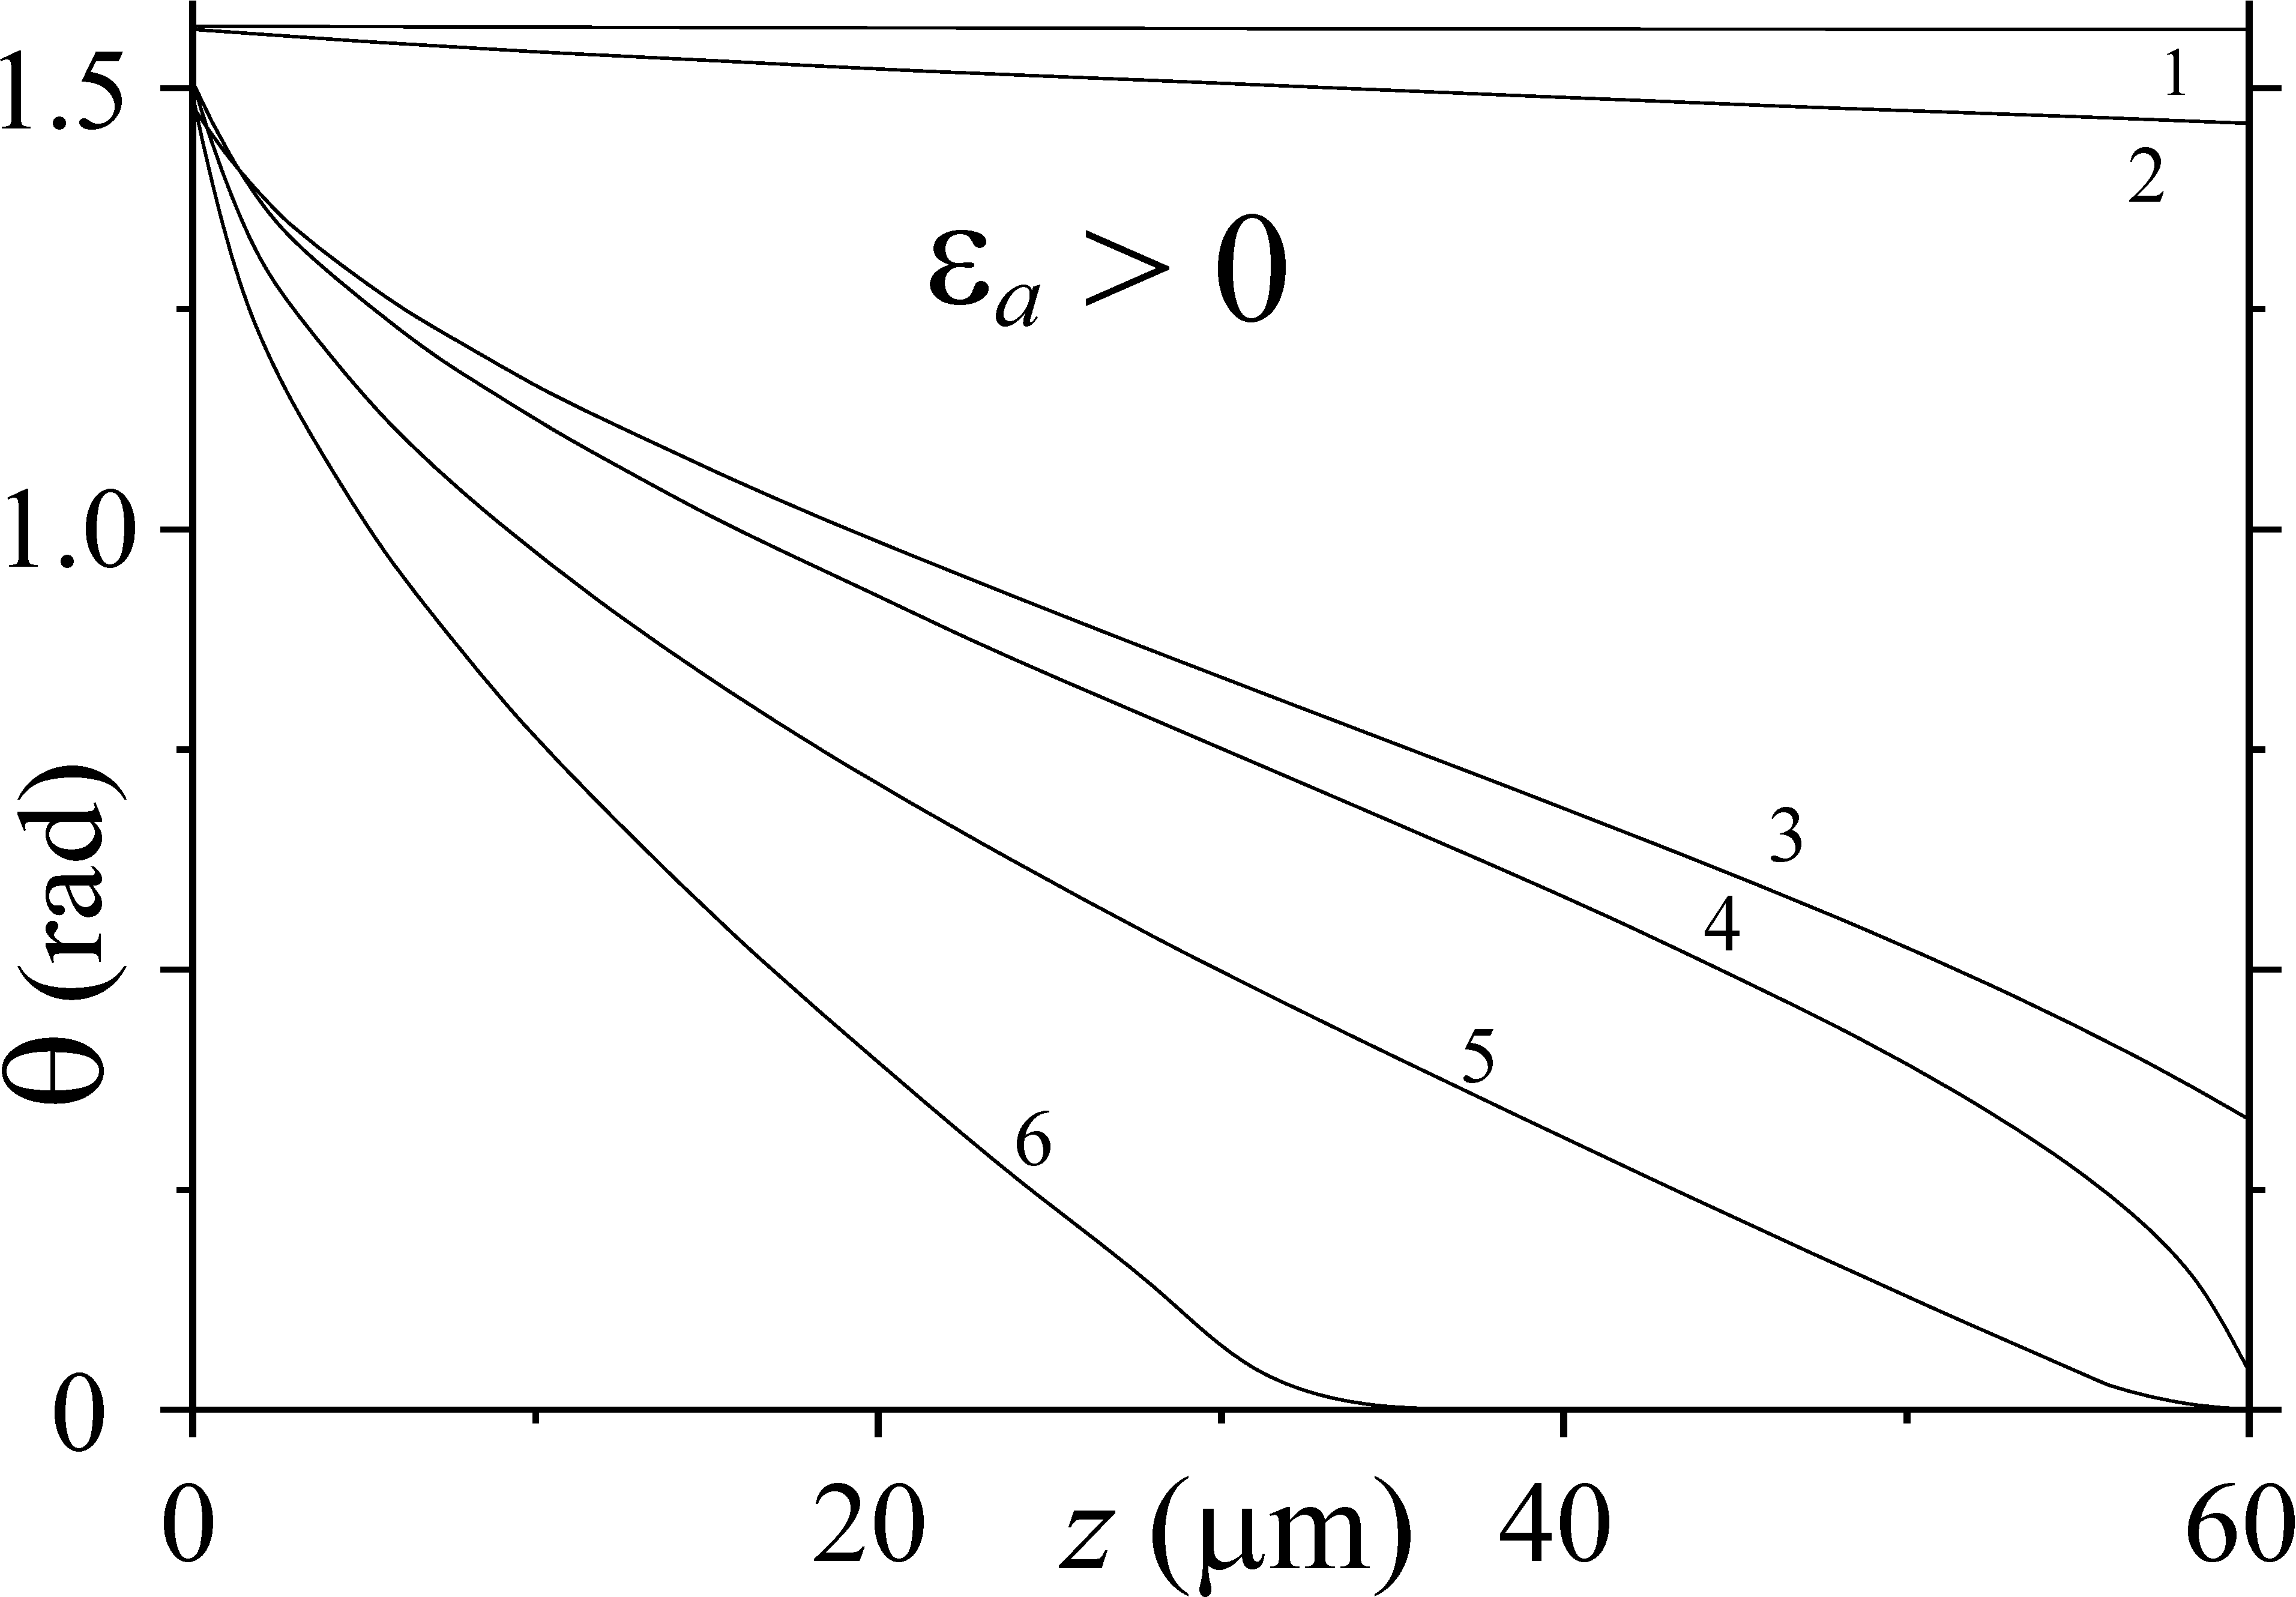
\includegraphics[width=0.49\textwidth]{Profiles_POSITIVE_EA_at_fixed_e_0_01_change_U.eps}
\caption{Равновесные профили $\theta(z)$ для $\bar{e}=0.01$~statC/cm. Линии в случае $\varepsilon_a<0$: 1 -- $U=0.15 ~V$, 2 -- $U = 0.17 ~V$, 3 -- $U = 0.18 ~V$, 4 -- $U = 1 ~V$, 5 -- $U = 2 ~V$, 6 -- $U = 5 ~V$ и 7 -- $U = 10 ~V$; линии в случае  $\varepsilon_a > 0$: 1 -- $U = 0.15 ~V$, 2 -- $U = 0.17 ~V$, 3 -- $U = 0.18 ~V$, 4 -- $U = 1 ~V$, 5 -- $U = 5 ~V$ и 6 -- $10 ~V$.}
\end{figure}
\end{frame}

\begin{frame}
\frametitle{Основные результаты}
%\framesubtitle{Сравнение прямой минимизации и аналитической}
\begin{enumerate}
\item Показано, что при $\varepsilon_a < 0$ переход Фредерикса возможен при достаточно большом $\bar{e}$, причём он может быть только непрерывным;
%\item Получено описание перехода Фредерикса с учётом неоднородности электрического поля, флексоэлектричества и мягкого зацепления границ для отрицательной диэлектрической анизотропии;
\item Было обнаружено, что для достаточно больших $\bar{e}$ напряжение перехода убывает как $1/\bar{e}$;
%\item Был обнаружен переход нового типа -- .
\item Было обнаружено, что при повышении напряжения выше перехода Фредерикса происходит ещё один переход -- из слабоискажённой фазы в сильноискажённую.
\end{enumerate}
\end{frame}

\begin{frame}
\centering
%\section{Text}
{\large Часть 3. Случай большого флексоэлектрического коэффициента и достаточно высокого приложенного напряжения\blfootnote{Результаты будут опубликованы в \textit{Journal of Physics: Conference Series}}}
\begin{equation}
\frac{\bar{e}U}{K} \gg 1
\end{equation}
\end{frame}

\begin{frame}
\frametitle{Большой $\bar{e}$ и высокое $U$}
\framesubtitle{Основные понятия}
\footnotesize
%\begin{block}{Критерий применимости}
%\begin{equation}
%\frac{\bar{e}U}{K} \gg 1
%\end{equation}
%\end{block}
\begin{block}{Свободная энергия}
\vspace{-0.5cm}
\begin{multline}
\frac{\FF_\mathrm{tot}}{S_\bot} = -\frac{1}{8\pi}U^2 J + \bar{e}UJJ_1 + 2\pi\bar{e}^2 \left( \int_0^L\frac{(\sin 2{\theta} \theta')^2}{\EE(\theta)}\ dz - JJ_1^2 \right) +\\
\frac{W_1}{2}\sin^2\left(\theta(0) - \theta_0^{(1)}\right) + \frac{W_2}{2}\sin^2\left(\theta(L) - \theta_0^{(2)}\right) + \mathrm{elastic}
\end{multline}
\end{block}
Обозначим $y(z) = \frac{\varepsilon_\bot}{\varepsilon_a} + \cos^2{\theta(z)}$, $y(z) \in \left[ \frac{\varepsilon_\bot}{\varepsilon_a};\ \frac{\varepsilon_\parallel}{\varepsilon_a} \right]\ \forall z \in [0;\ L]$
\begin{block}{Свободная энергия как функционал $y(z)$}
\vspace{-0.5cm}
\begin{multline}
\frac{\FF_\mathrm{tot}}{S_\bot} = -\frac{1}{8\pi}U^2 J + \bar{e}UJJ_1 + 2\pi\bar{e}^2 \left( \frac{1}{\varepsilon_a}\int_0^L\frac{(y')^2}{y(z)}\ dz - JJ_1^2 \right) +\\
 + \frac{W_1}{2}y(0) + \frac{W_2}{2}y(L) + \mathrm{elastic}
\end{multline}
\end{block}
\begin{block}{Reminder}
\begin{equation}
J^{-1} =\frac{1}{\varepsilon_a}\int_0^L \frac{dz}{y(z)}, \quad J_1 = \frac{1}{\varepsilon_a} \ln \frac{y(0)}{y(L)}
\end{equation}
\end{block}
\end{frame}


\begin{frame}
\frametitle{Большой $\bar{e}$ и высокое $U$}
\framesubtitle{Вариационный принцип}
\begin{block}{Вариация в объёме}
\begin{equation}
\frac{\delta \FF}{S_\bot\delta y(z)} = \frac{2\pi\bar{e}^2}{\varepsilon_a y^2}\left[ -2yy'' + (y')^2 - a^2 \right]
\end{equation}
\end{block}
\begin{block}{Уравнение Эйлера-Лагранжа в объёме}
\begin{equation}
-2yy'' + (y')^2 - a^2 = 0
\end{equation}
\end{block}
Здесь
\begin{equation}
a \equiv J\left(J_1 - \frac{U}{4\pi \bar{e}}\right)
\end{equation}
\begin{block}{Reminder}
\begin{equation}
J^{-1} =\frac{1}{\varepsilon_a}\int_0^L \frac{dz}{y(z)}, \quad J_1 = \frac{1}{\varepsilon_a} \ln \frac{y(0)}{y(L)}
\end{equation}
\end{block}
\end{frame}



\begin{frame}
\frametitle{Большой $\bar{e}$ и высокое $U$}
\framesubtitle{Решение уравнения в объёме}
\begin{block}{Решения}
\begin{align}
&y(z) = \pm az + b, \\
&y(z) = \frac{c}{4} \left(z + b\right)^2 - \frac{a^2}{c}
\end{align}
Произвольные константы: $b, c$
\end{block}
\end{frame}

\begin{frame}
\frametitle{Большой $\bar{e}$ и высокое $U$}
\framesubtitle{Вариация на границах}
\small
\begin{block}{Вариация на границах}
\vspace{-0.5cm}
\begin{align}
&\frac{\delta \FF}{S_\bot\delta y(0)} = \frac{4\pi\bar{e}^2}{\varepsilon_a y(0)}\left[ -y'(0) - a + g_1 y(0) \right] \alert{(=0)}\\
&\frac{\delta \FF}{S_\bot\delta y(L)} = \frac{4\pi\bar{e}^2}{\varepsilon_a y(L)}\left[ y'(0) + a + g_2 y(0) \right] \alert{(=0)}
\end{align}
\begin{equation}
g_i \equiv \frac{\varepsilon_a W_i}{8\pi\bar{e}^2}
\end{equation}
\end{block}
\begin{figure}
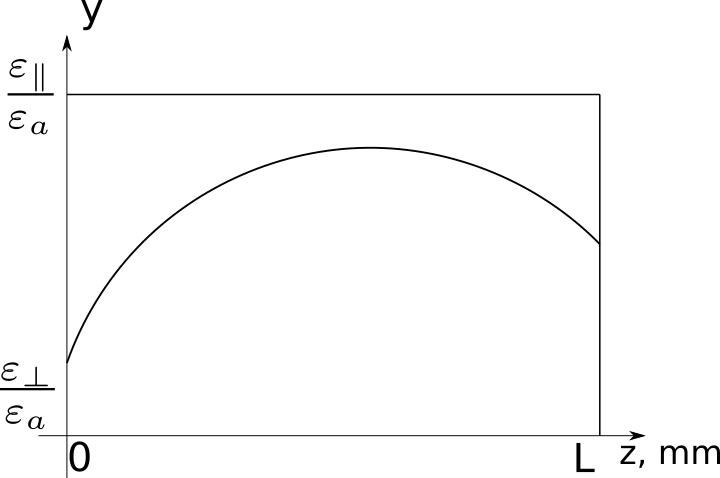
\includegraphics[width = 0.4\textwidth]{Profile_basic_impossible.png}
\vspace{-0.2cm}
\caption{Профилей такого вида не существует}
\end{figure}
\end{frame}



\begin{frame}
\frametitle{Большой $\bar{e}$ и высокое $U$}
\framesubtitle{Пояснение к вариационному принципу}
\begin{block}{Формальное требование на экстремаль}
$$
\delta \FF \geq 0
$$
для любых \alert{допустимых} $\delta y(z)$.
\end{block}
\begin{block}{Ограниченность функции}
$$
y(z) \in \left[ \frac{\varepsilon_\bot}{\varepsilon_a};\ \frac{\varepsilon_\parallel}{\varepsilon_a} \right]\ \forall z \in [0;\ L]
$$
\end{block}
\begin{figure}[ht]
\centering
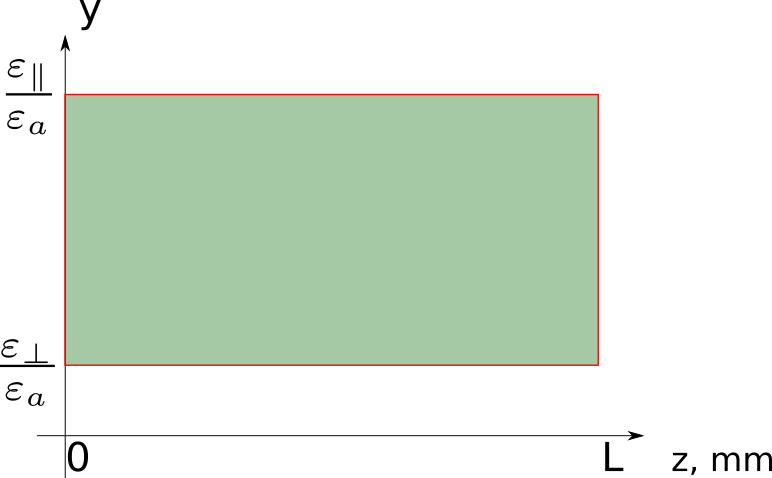
\includegraphics[width=5cm]{Sample_rectangle.png}
%\caption{Визуализация ограниченности $y(z)$}
\end{figure}
\end{frame}






\begin{frame}
\frametitle{Большой $\bar{e}$ и высокое $U$}
\framesubtitle{Профили без участков насыщения}
\vspace{-0.25cm}
\begin{figure}[ht]
\centering
\begin{minipage}{0.49\textwidth}
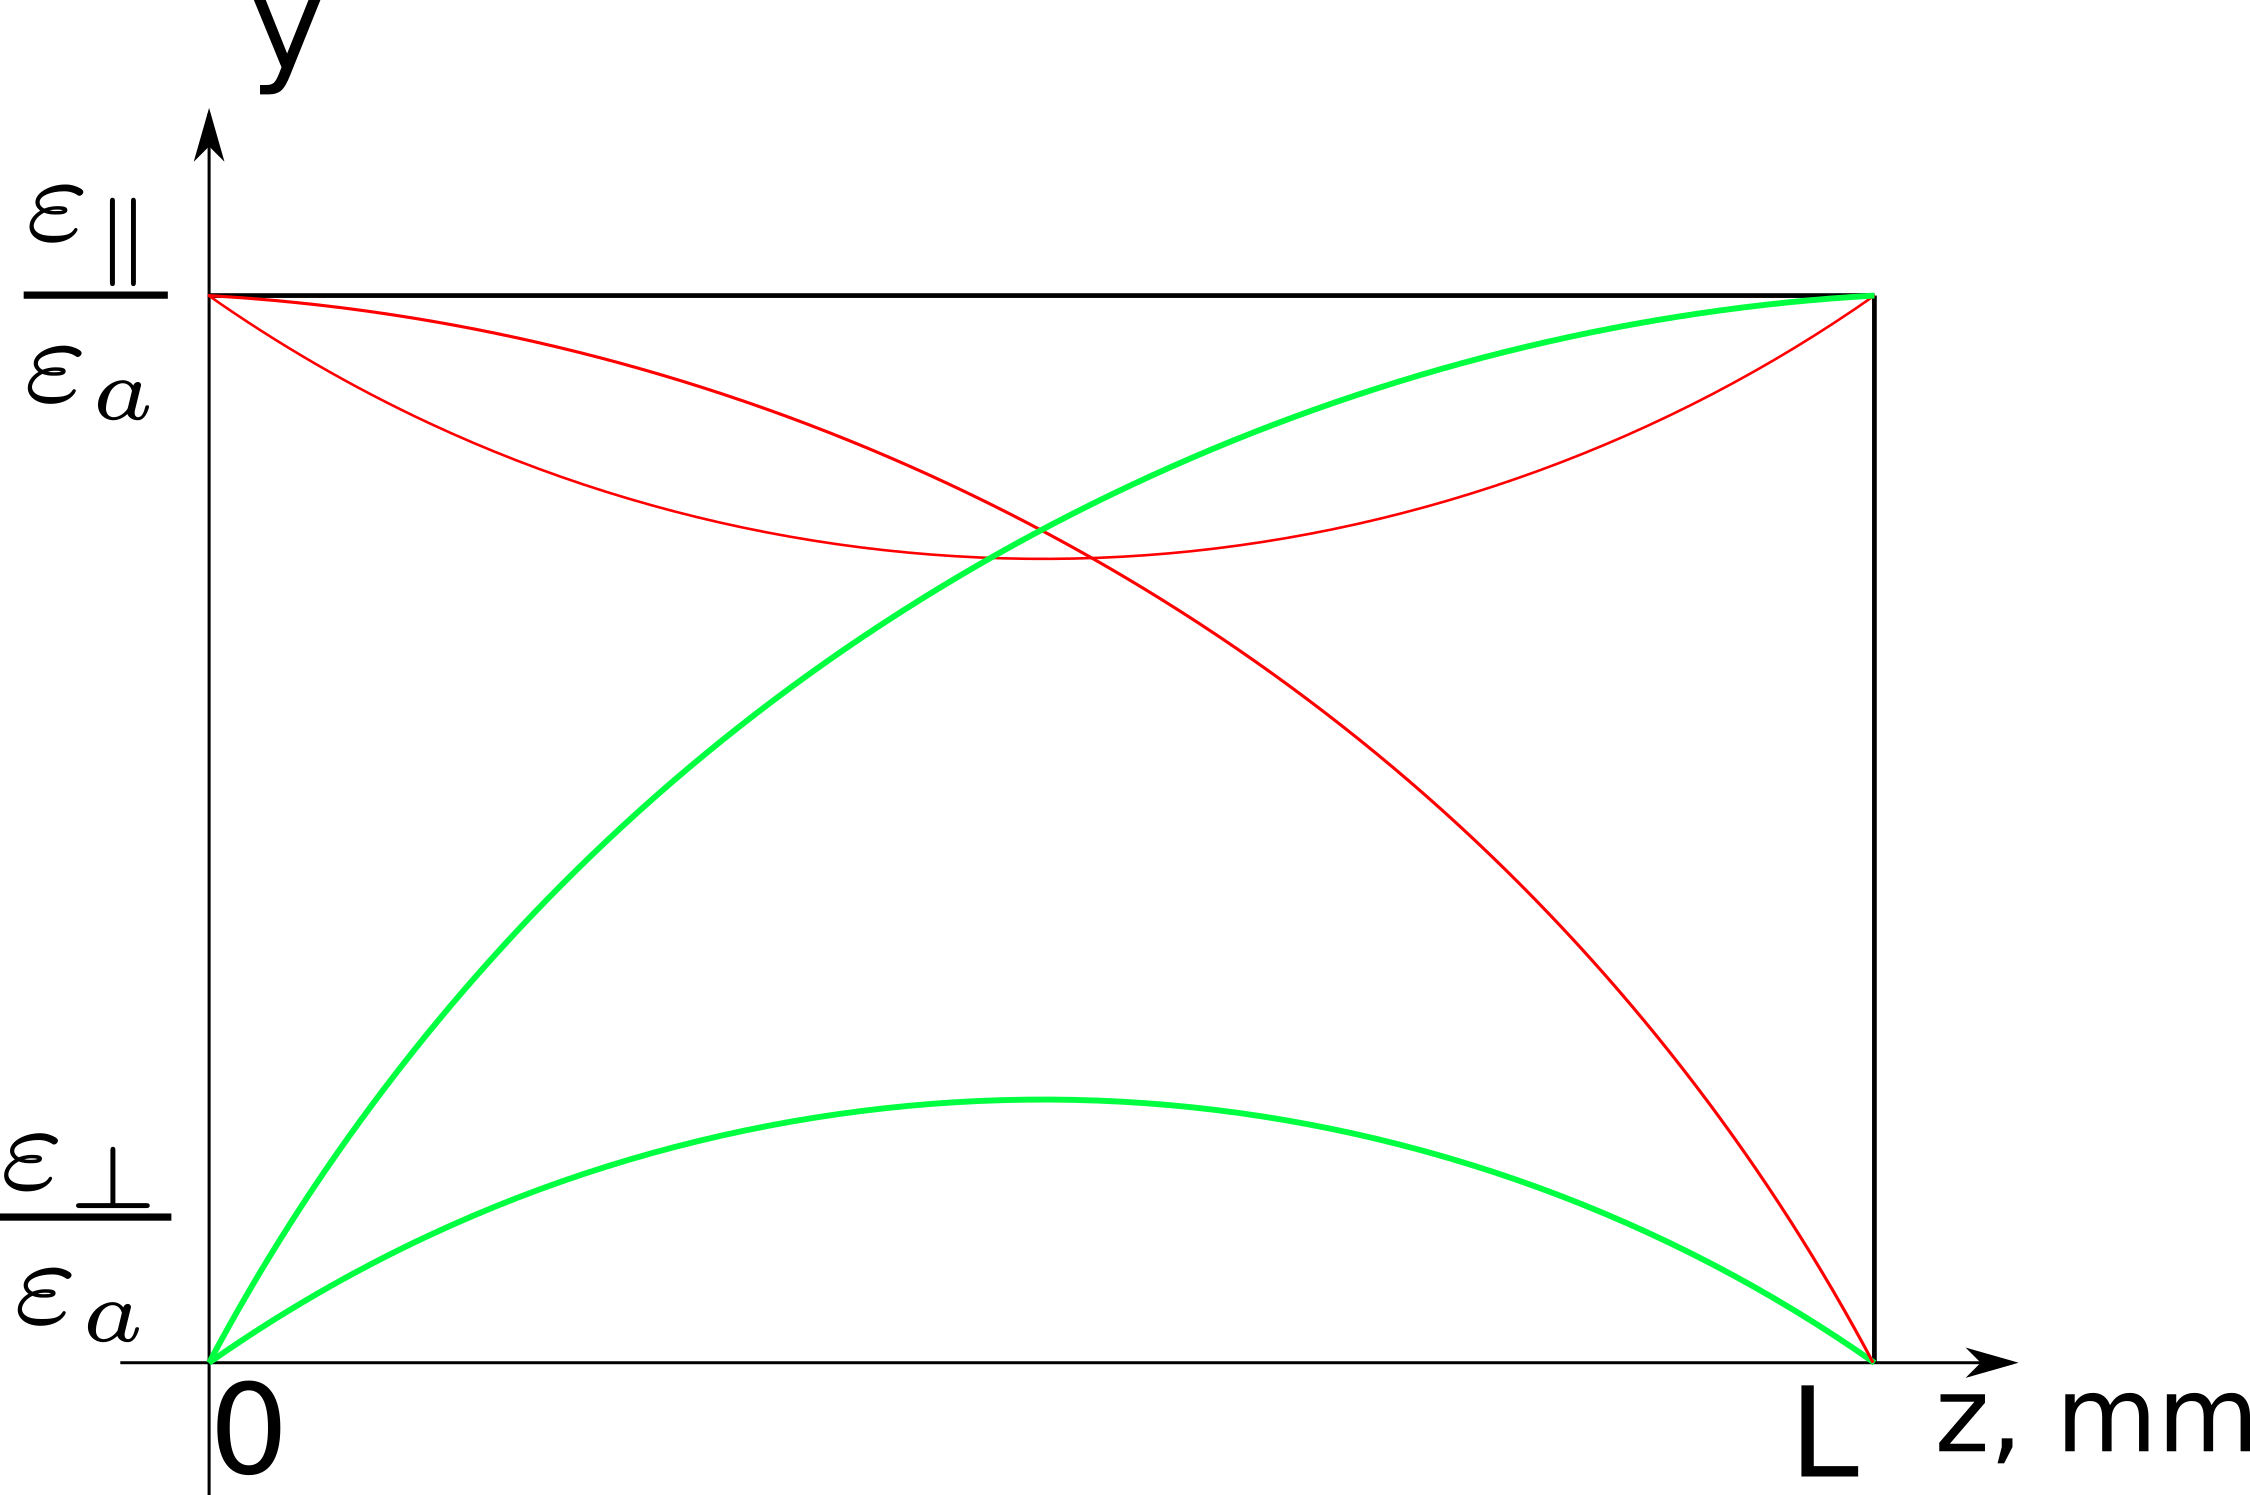
\includegraphics[width=\textwidth]{Profiles_corners.png}
\end{minipage}
\hfill
\begin{minipage}{0.49\textwidth}
\caption{Примеры профилей с концами в углах}
\end{minipage}
\end{figure}
\vspace{-0.25cm}
\begin{figure}[ht]
\centering
\begin{minipage}{0.49\textwidth}
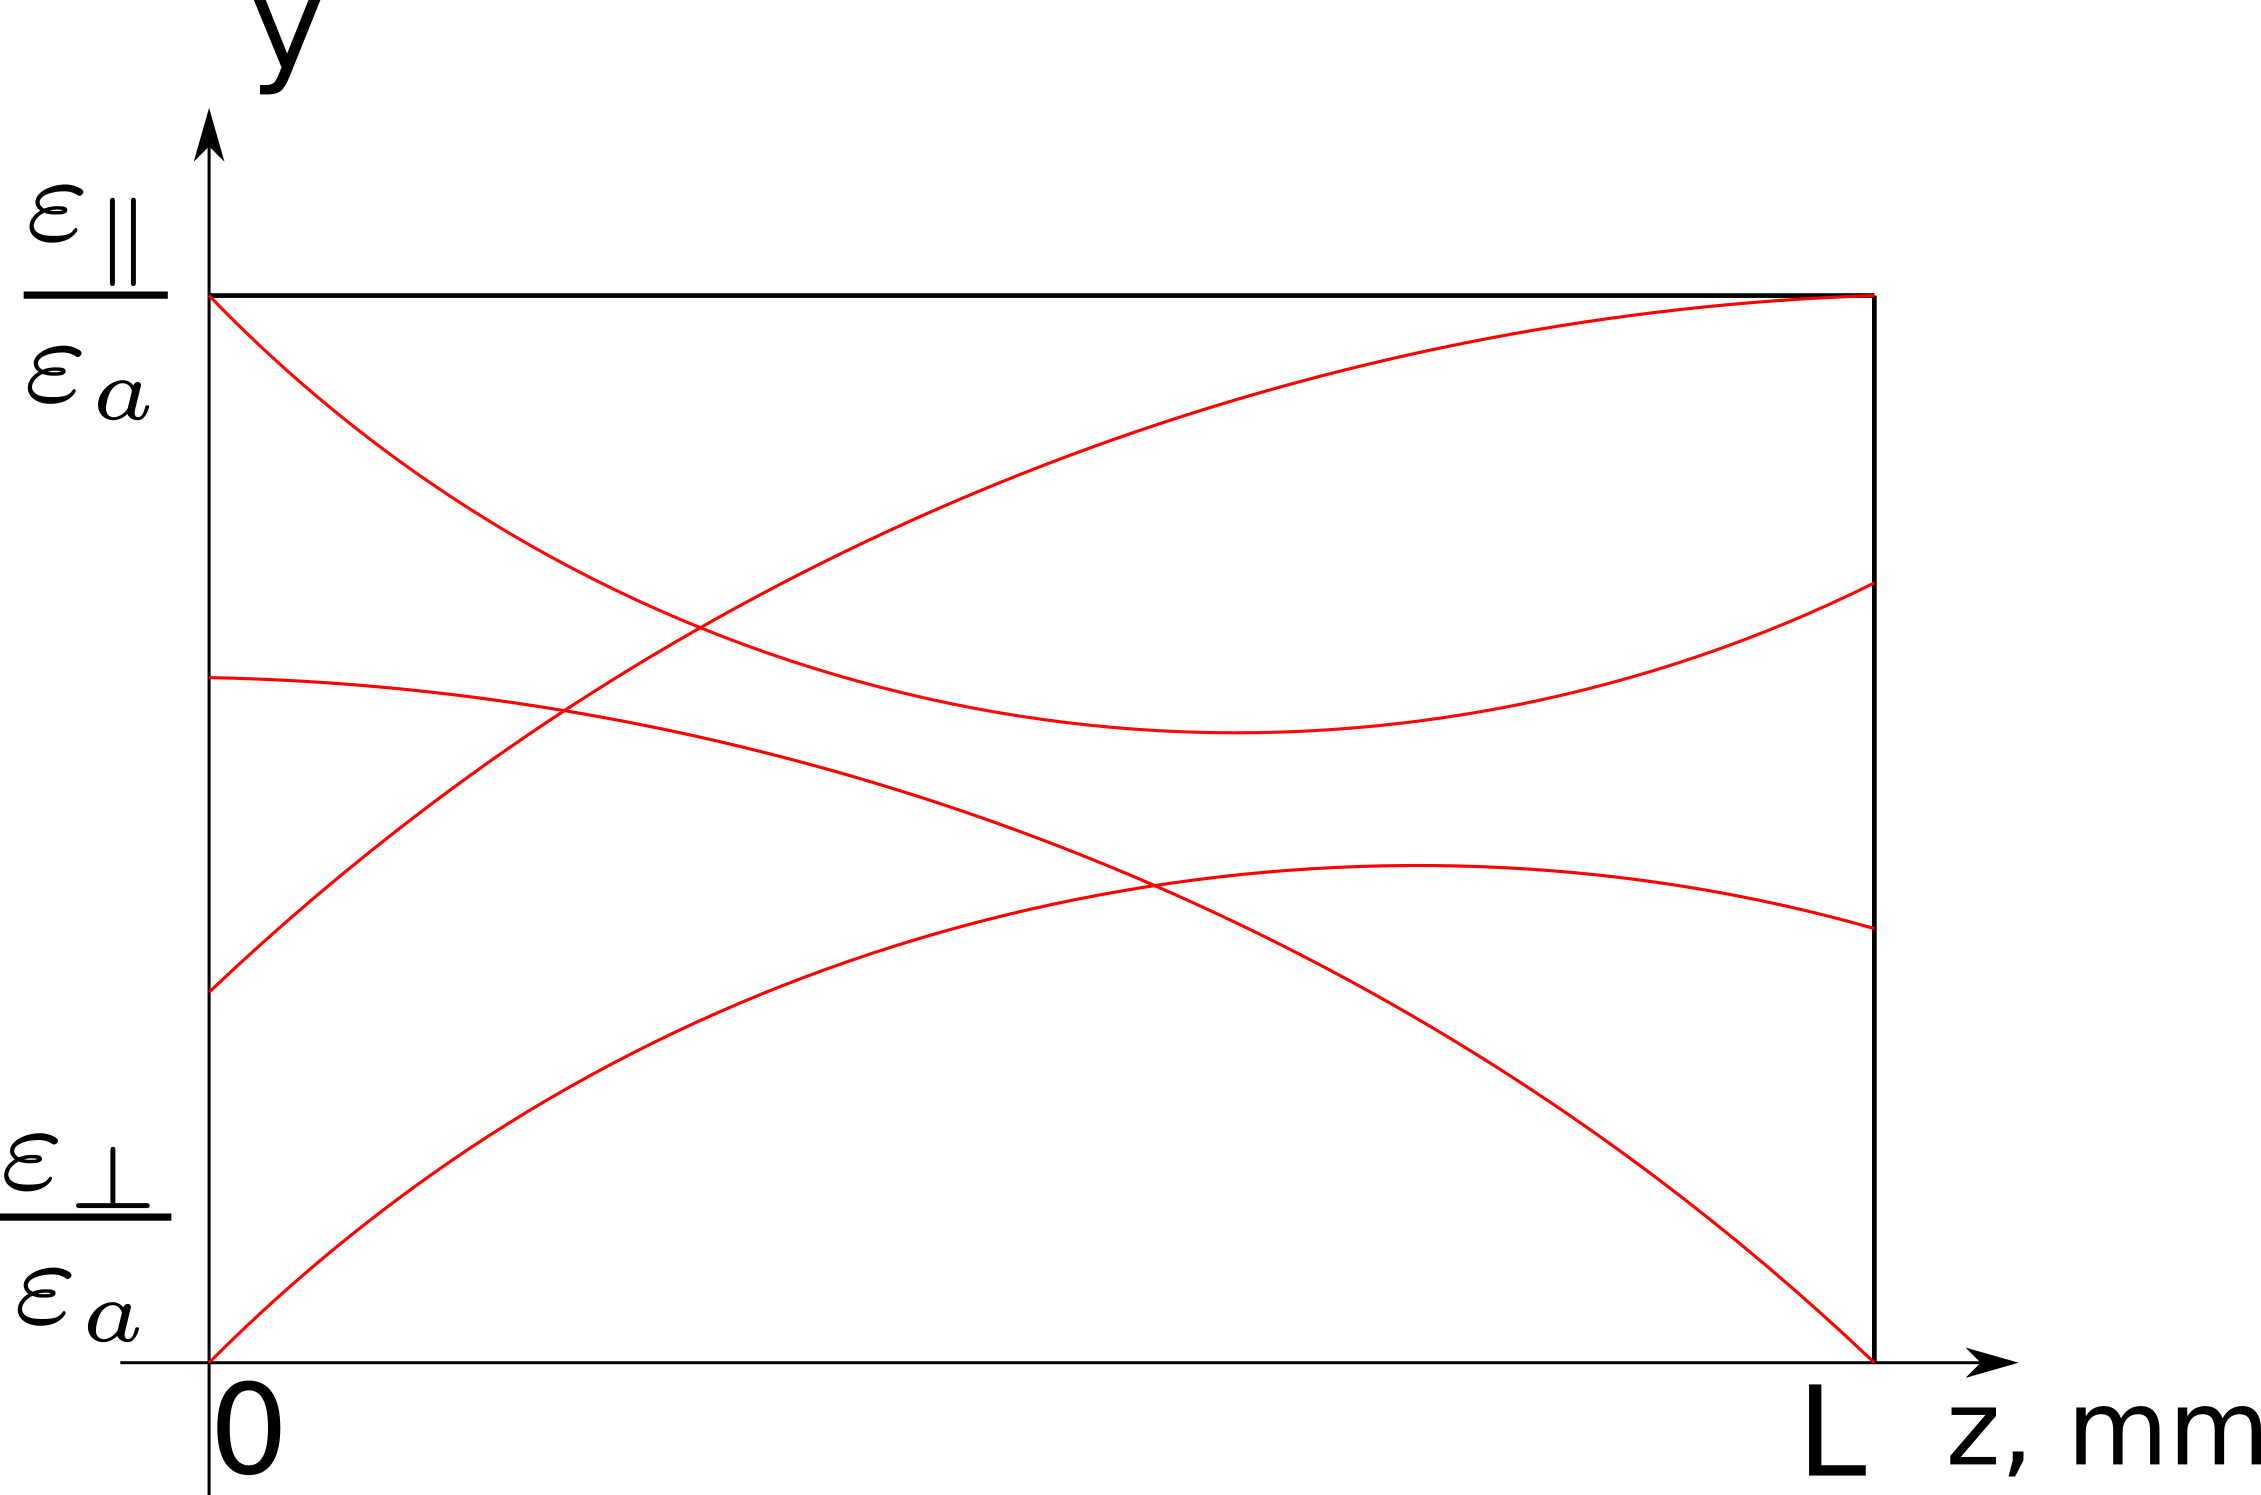
\includegraphics[width=\textwidth]{Profiles_corners_and_sides.png}
\end{minipage}
\hfill
\begin{minipage}{0.49\textwidth}
\caption{Примеры профилей, у которых только один конец находится в углу.}
\end{minipage}
\end{figure}
\end{frame}

%\begin{frame}
%\frametitle{Большой $\bar{e}$ и высокое $U$}
%\framesubtitle{Профили без участков насыщения}
%\begin{figure}[ht]
%\centering
%\begin{minipage}{0.49\textwidth}
%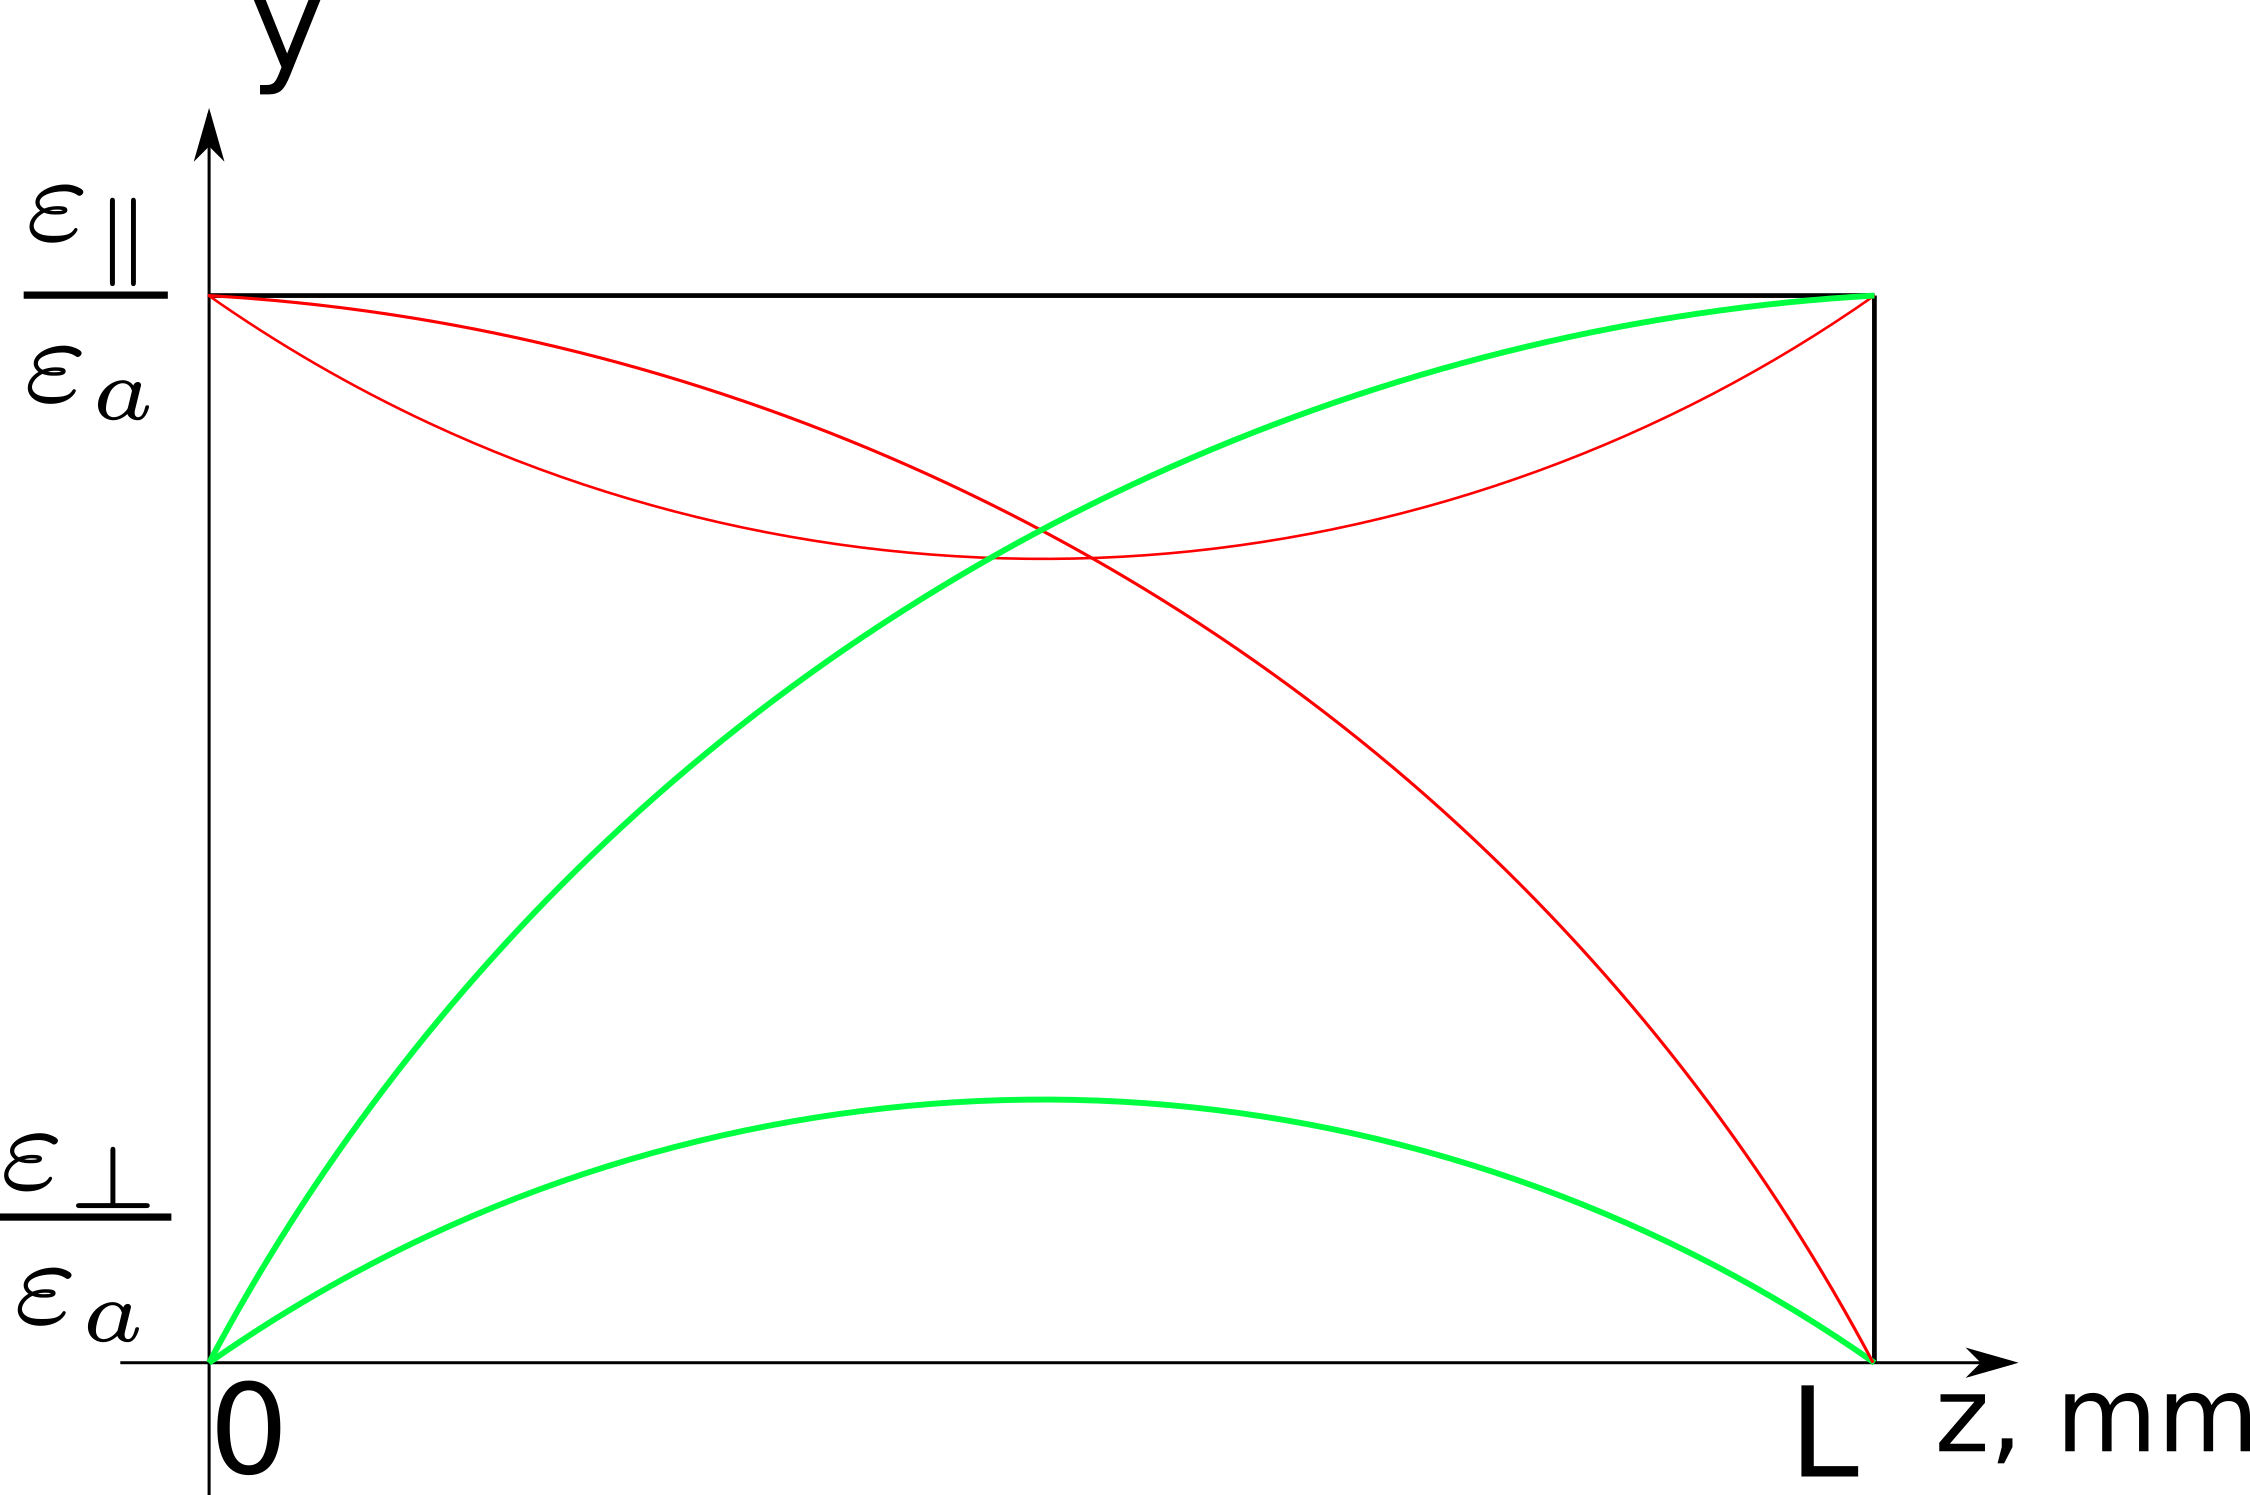
\includegraphics[width=\textwidth]{Profiles_corners.png}
%\caption{Примеры профилей с концами в углах}
%\end{minipage}
%\hfil
%\begin{minipage}{0.49\textwidth}
%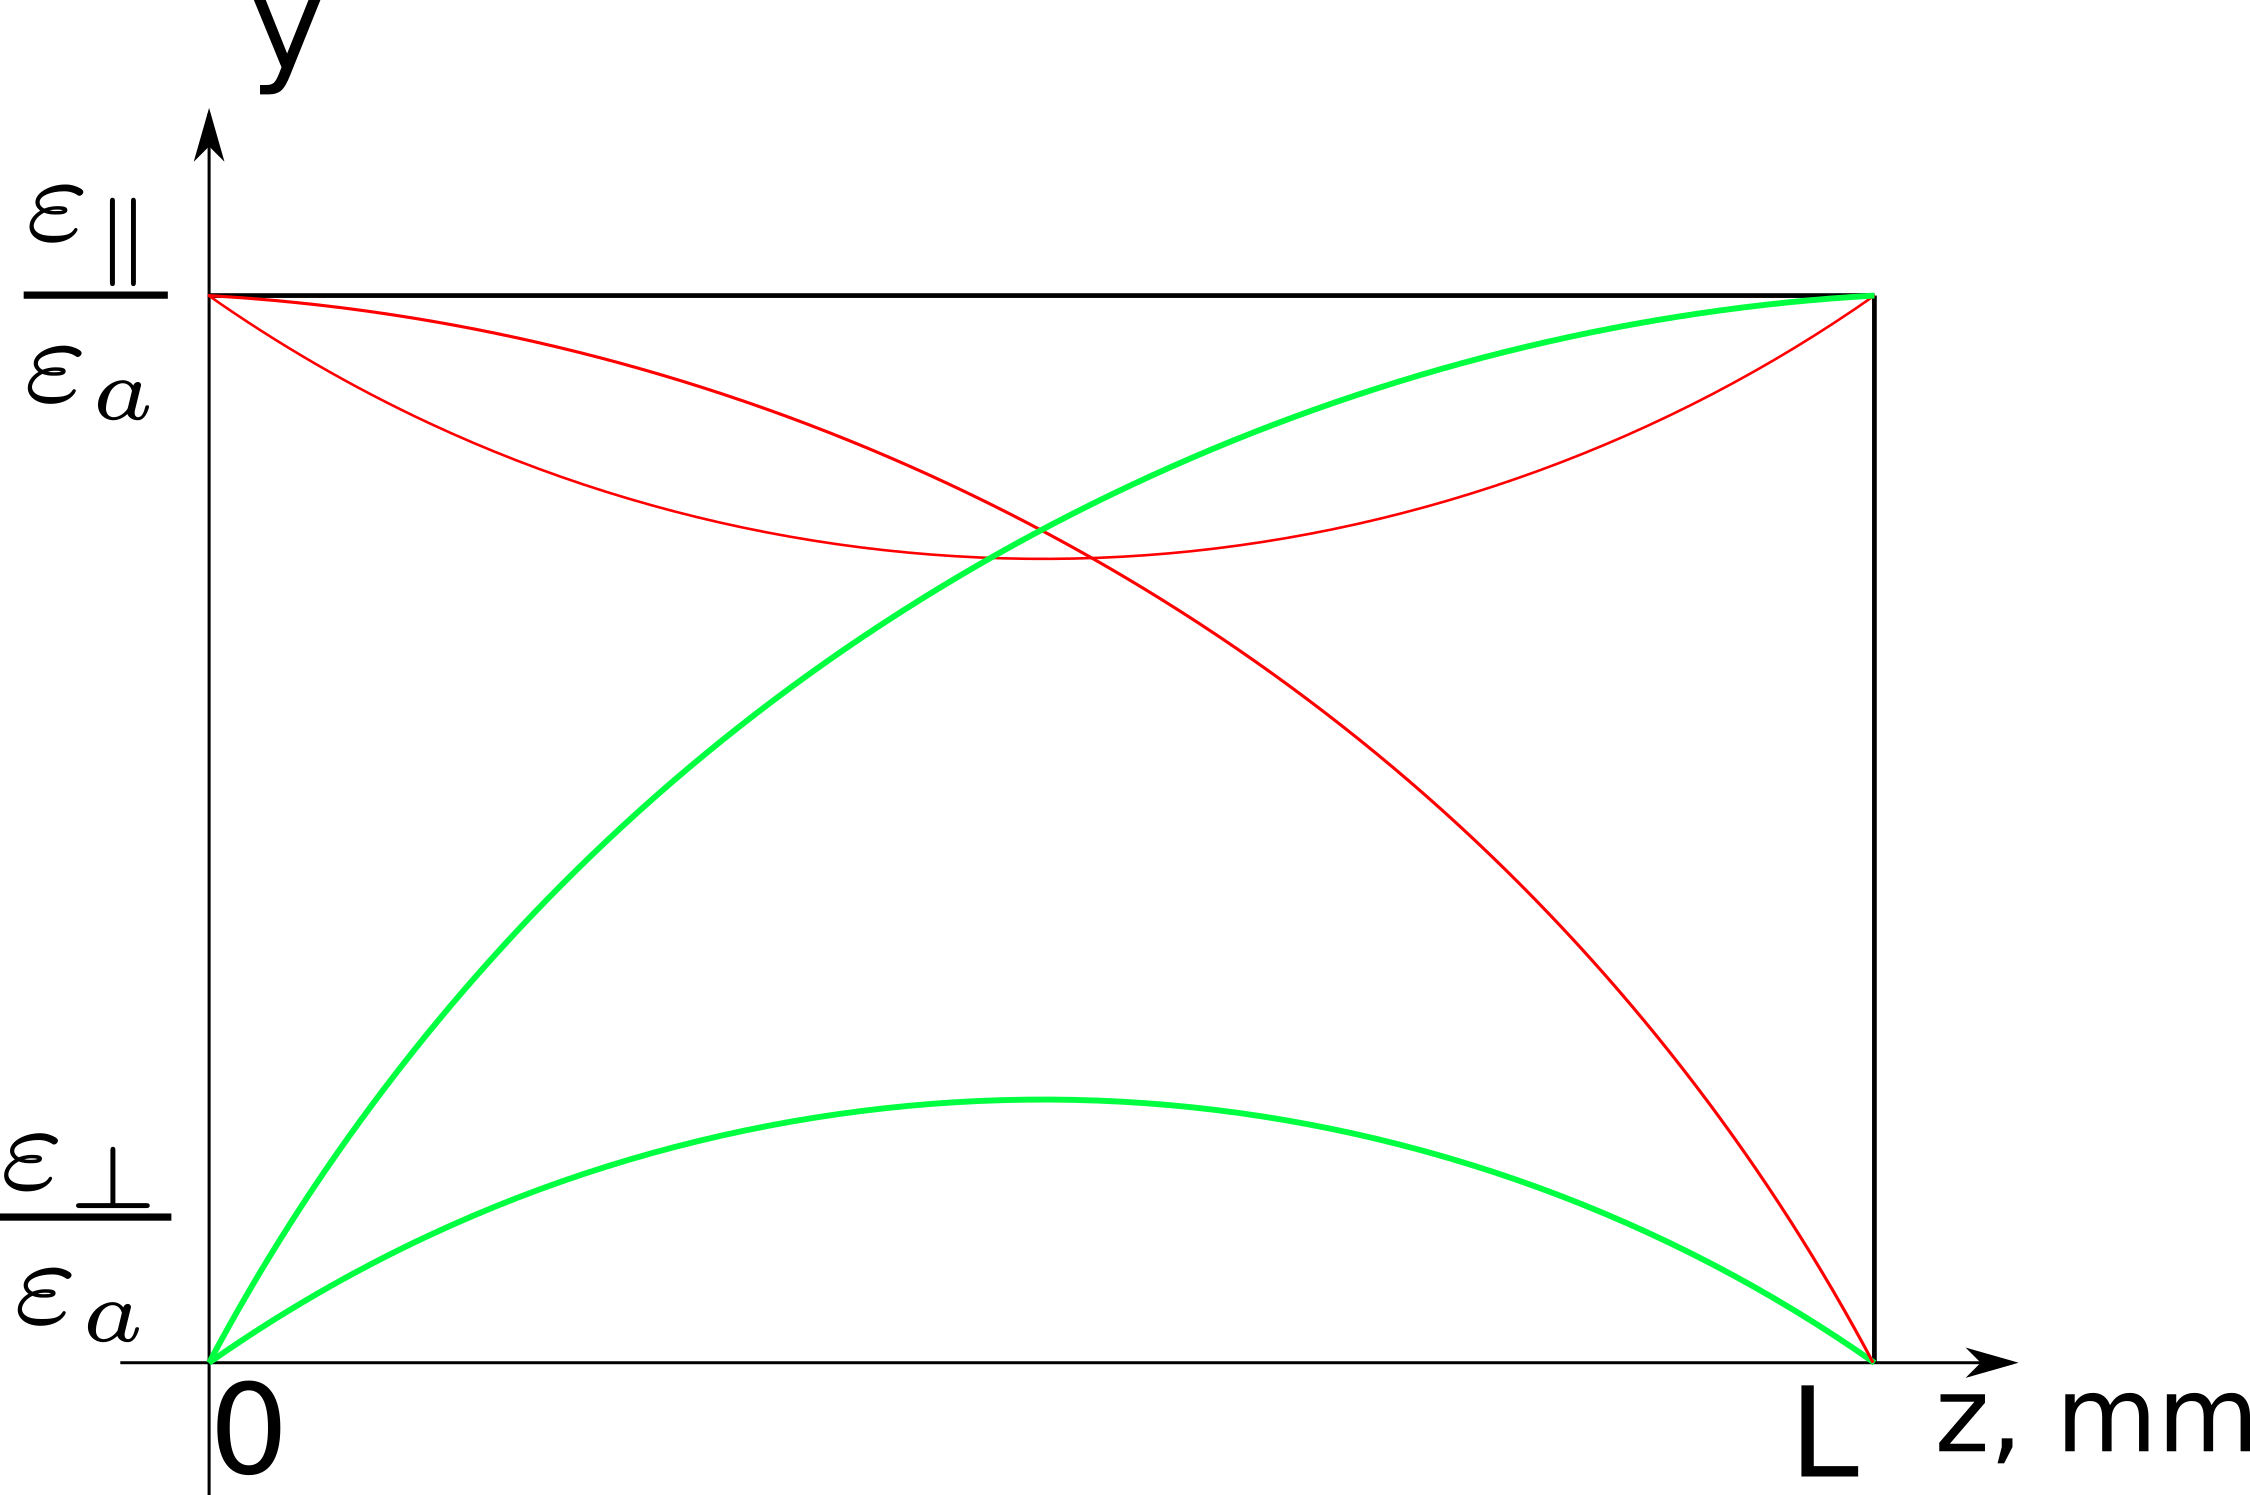
\includegraphics[width=\textwidth]{Profiles_corners.png}
%\caption{Примеры профилей, у которых только один конец находится в углу}
%\end{minipage}
%\end{figure}
%\end{frame}


\begin{frame}
\frametitle{Большой $\bar{e}$ и высокое $U$}
\framesubtitle{Процедура проверки возможности существования профилей}
\begin{block}{Условия существования профиля}
\begin{enumerate}
\item ``Геометрические'' условия: нужные точки находятся в углах, а сам профиль -- в прямоугольнике $[0;\,L] \times [\varepsilon_\bot/\varepsilon_a;\,\varepsilon_\parallel/\varepsilon_a]$
\item Неотрицательность первой вариации $\delta \FF / \delta y \geq 0$, в том числе на границах
\item Самосогласование: $a = J(J_1 - U/(4\pi\bar{e}))$
\end{enumerate}
\end{block}
Данные условия позволяют найти уравнение профиля, а также условия на параметры системы, при которых он существует. Данная задача сводится к обобщению условий Куна-Таккера на бесконечномерный случай. 
\end{frame}


\begin{frame}
\frametitle{Большой $\bar{e}$ и высокое $U$}
\framesubtitle{Какие профили возможны?}
\begin{block}{О насыщении}
\begin{equation}
\frac{\delta \FF}{S_\bot\delta y(z)} = \frac{2\pi\bar{e}^2}{\varepsilon_a y^2}\left[ -2yy'' + (y')^2 - a^2 \right]
\end{equation}
Вывод: при $\varepsilon_a > 0$ насыщение в объёме возможно лишь на $y = \varepsilon_\parallel / \varepsilon_a$
\end{block}
\end{frame}


\begin{frame}
\frametitle{Большой $\bar{e}$ и высокое $U$}
\framesubtitle{Профили с участками насыщения}
\vspace{-0.25cm}
\begin{figure}[ht]
\centering
\begin{minipage}{0.49\textwidth}
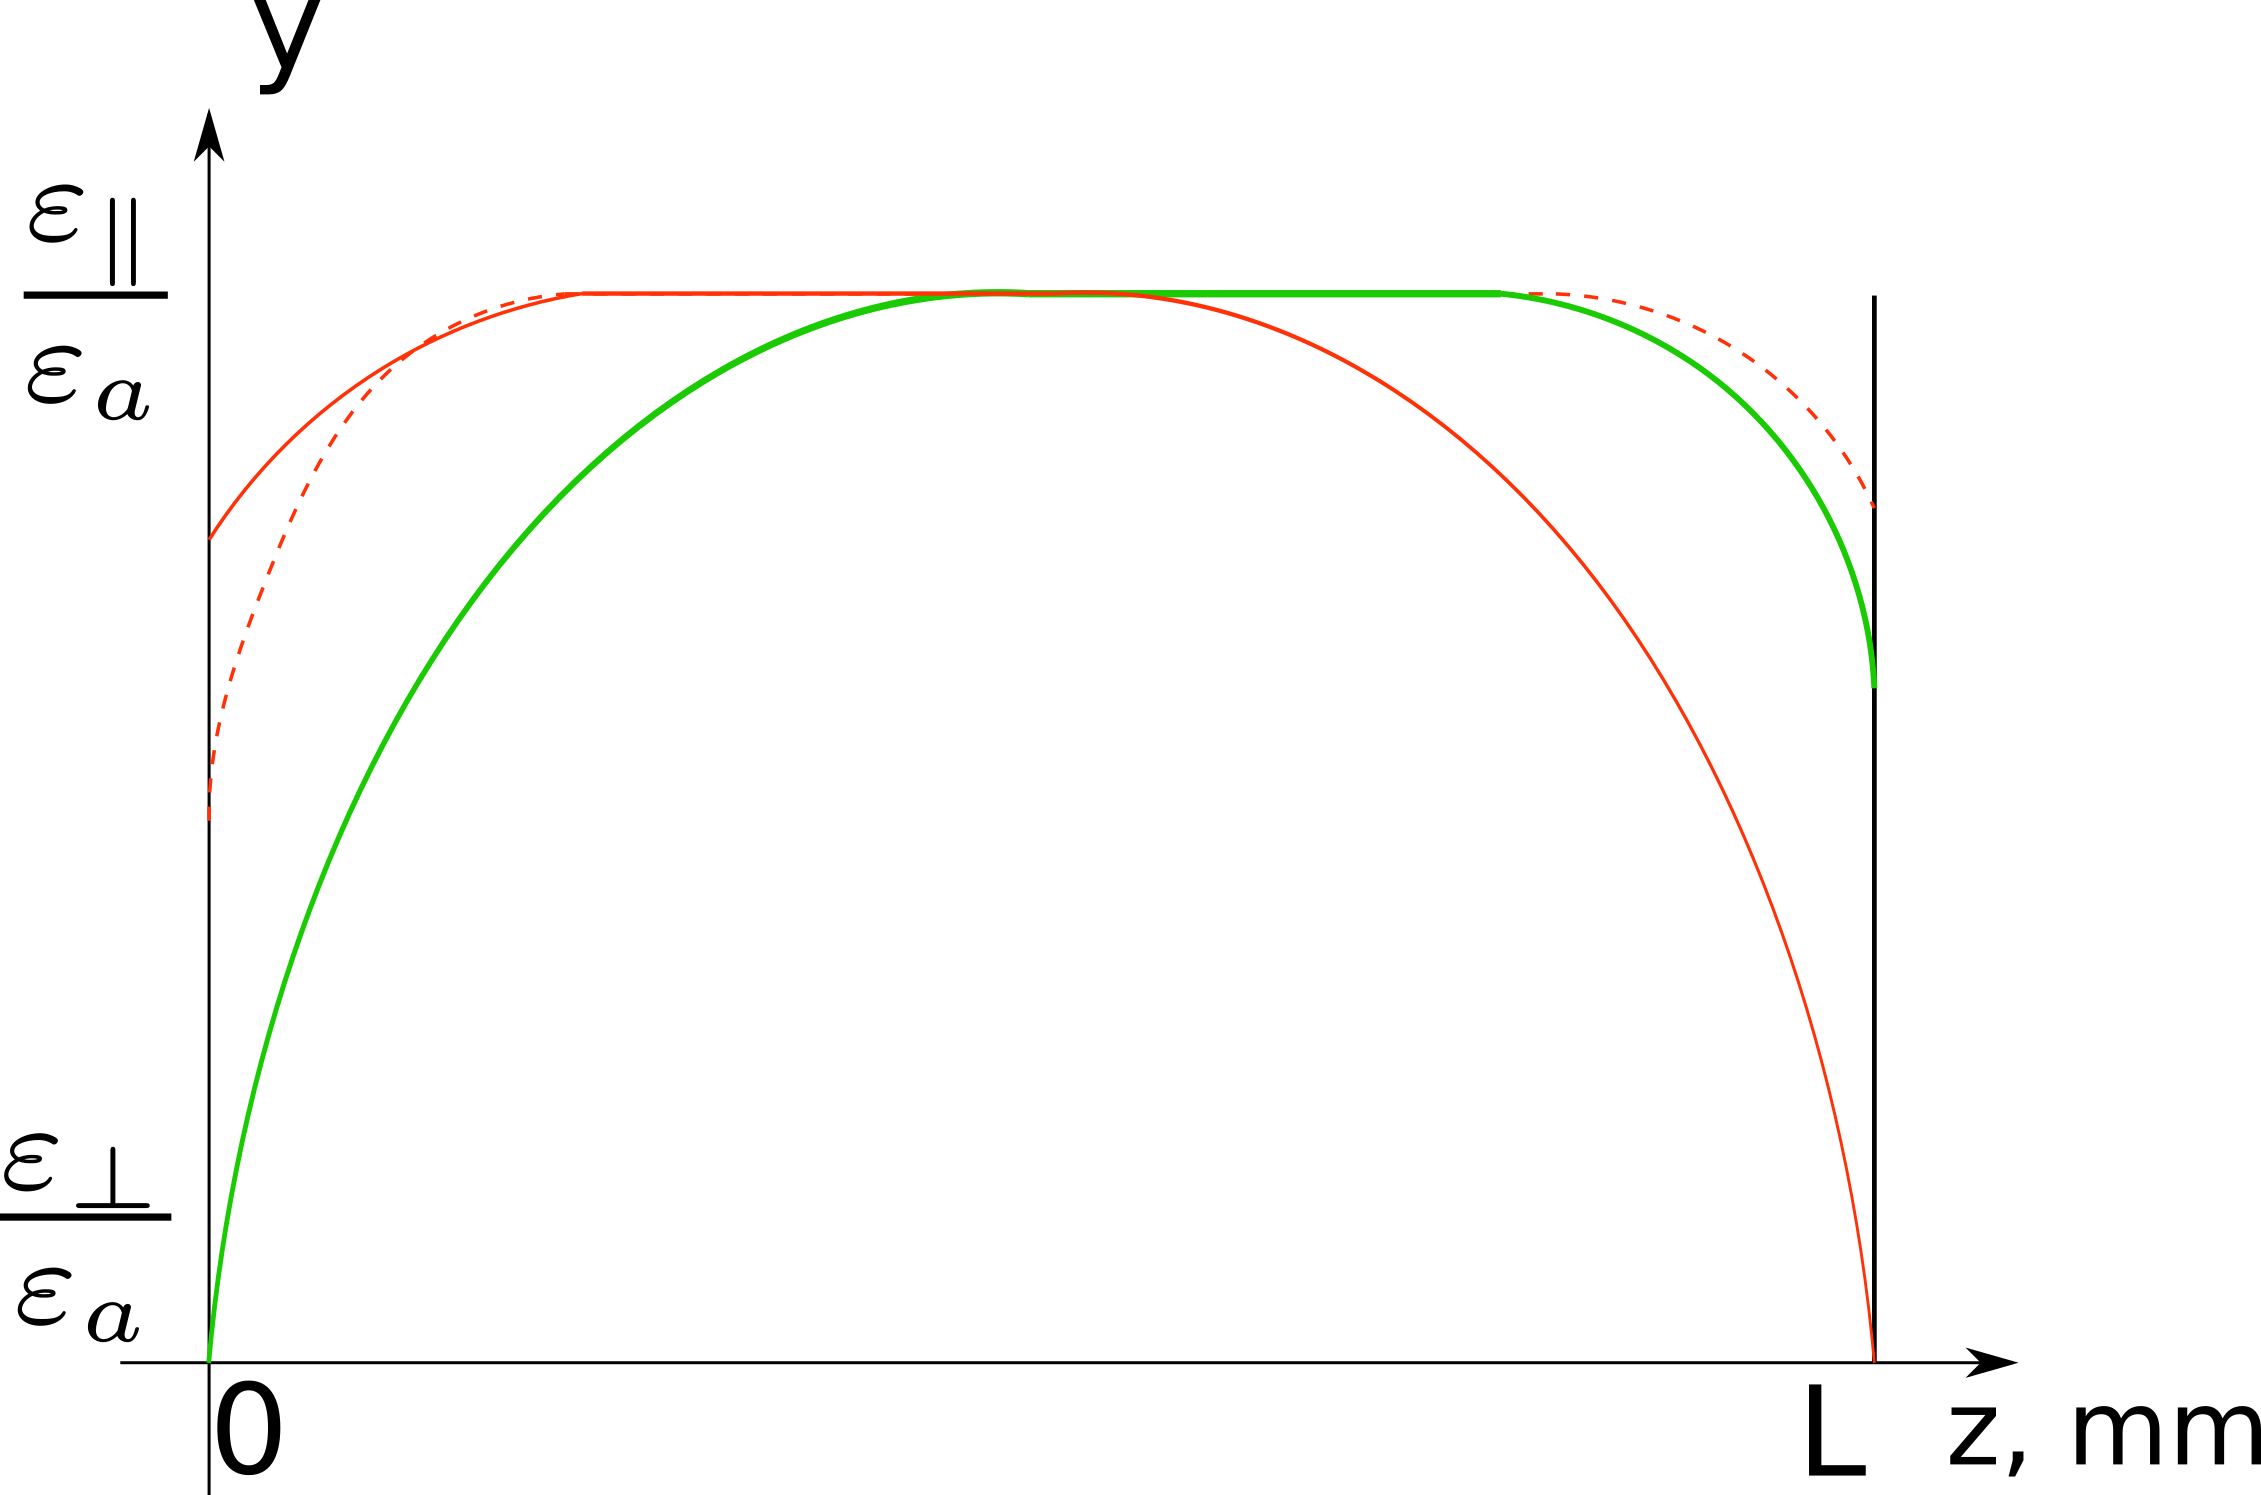
\includegraphics[width=\textwidth]{Profiles_saturated_1.png}
\end{minipage}
\hfill
\begin{minipage}{0.49\textwidth}
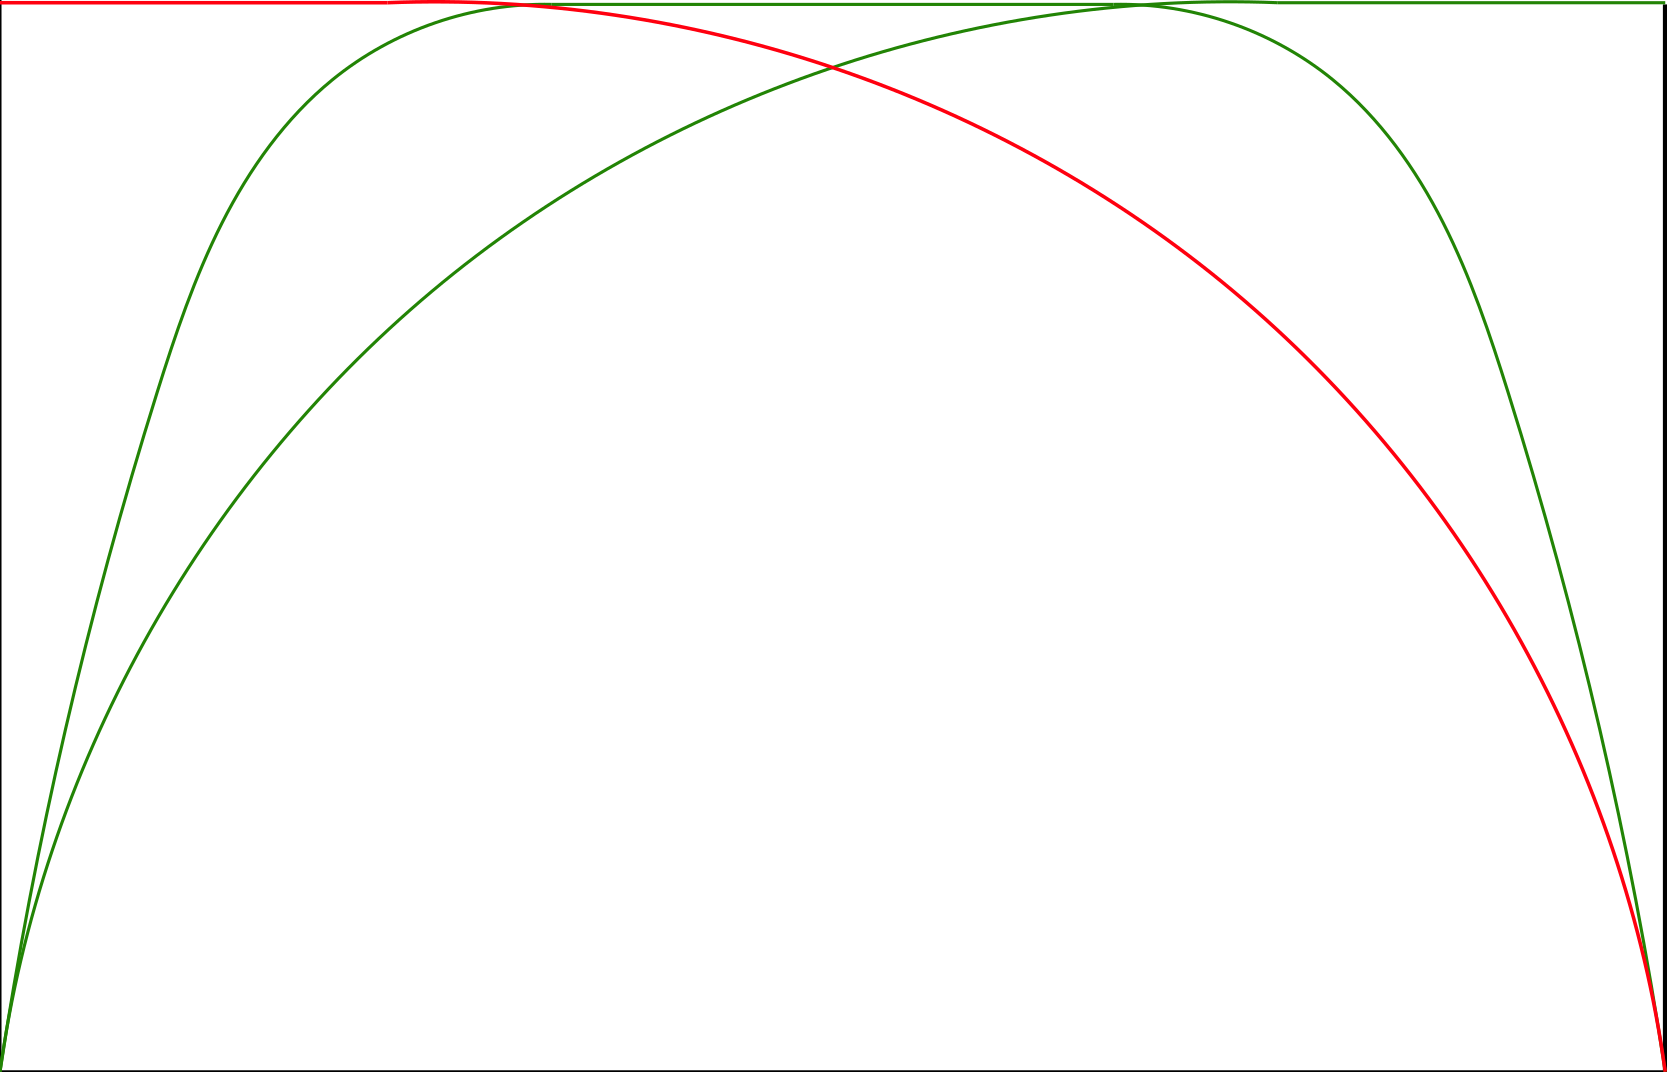
\includegraphics[width=\textwidth]{Profiles_saturated_2.png}
\end{minipage}
\caption{Варианты профилей с участками насыщения}
\end{figure}
\end{frame}



%
%\begin{frame}
%\frametitle{Большой $\bar{e}$ и высокое $U$}
%\framesubtitle{Пример проверки профиля}
%\vspace{-0.3cm}
%\begin{minipage}{0.51\textwidth}
%\begin{figure}
%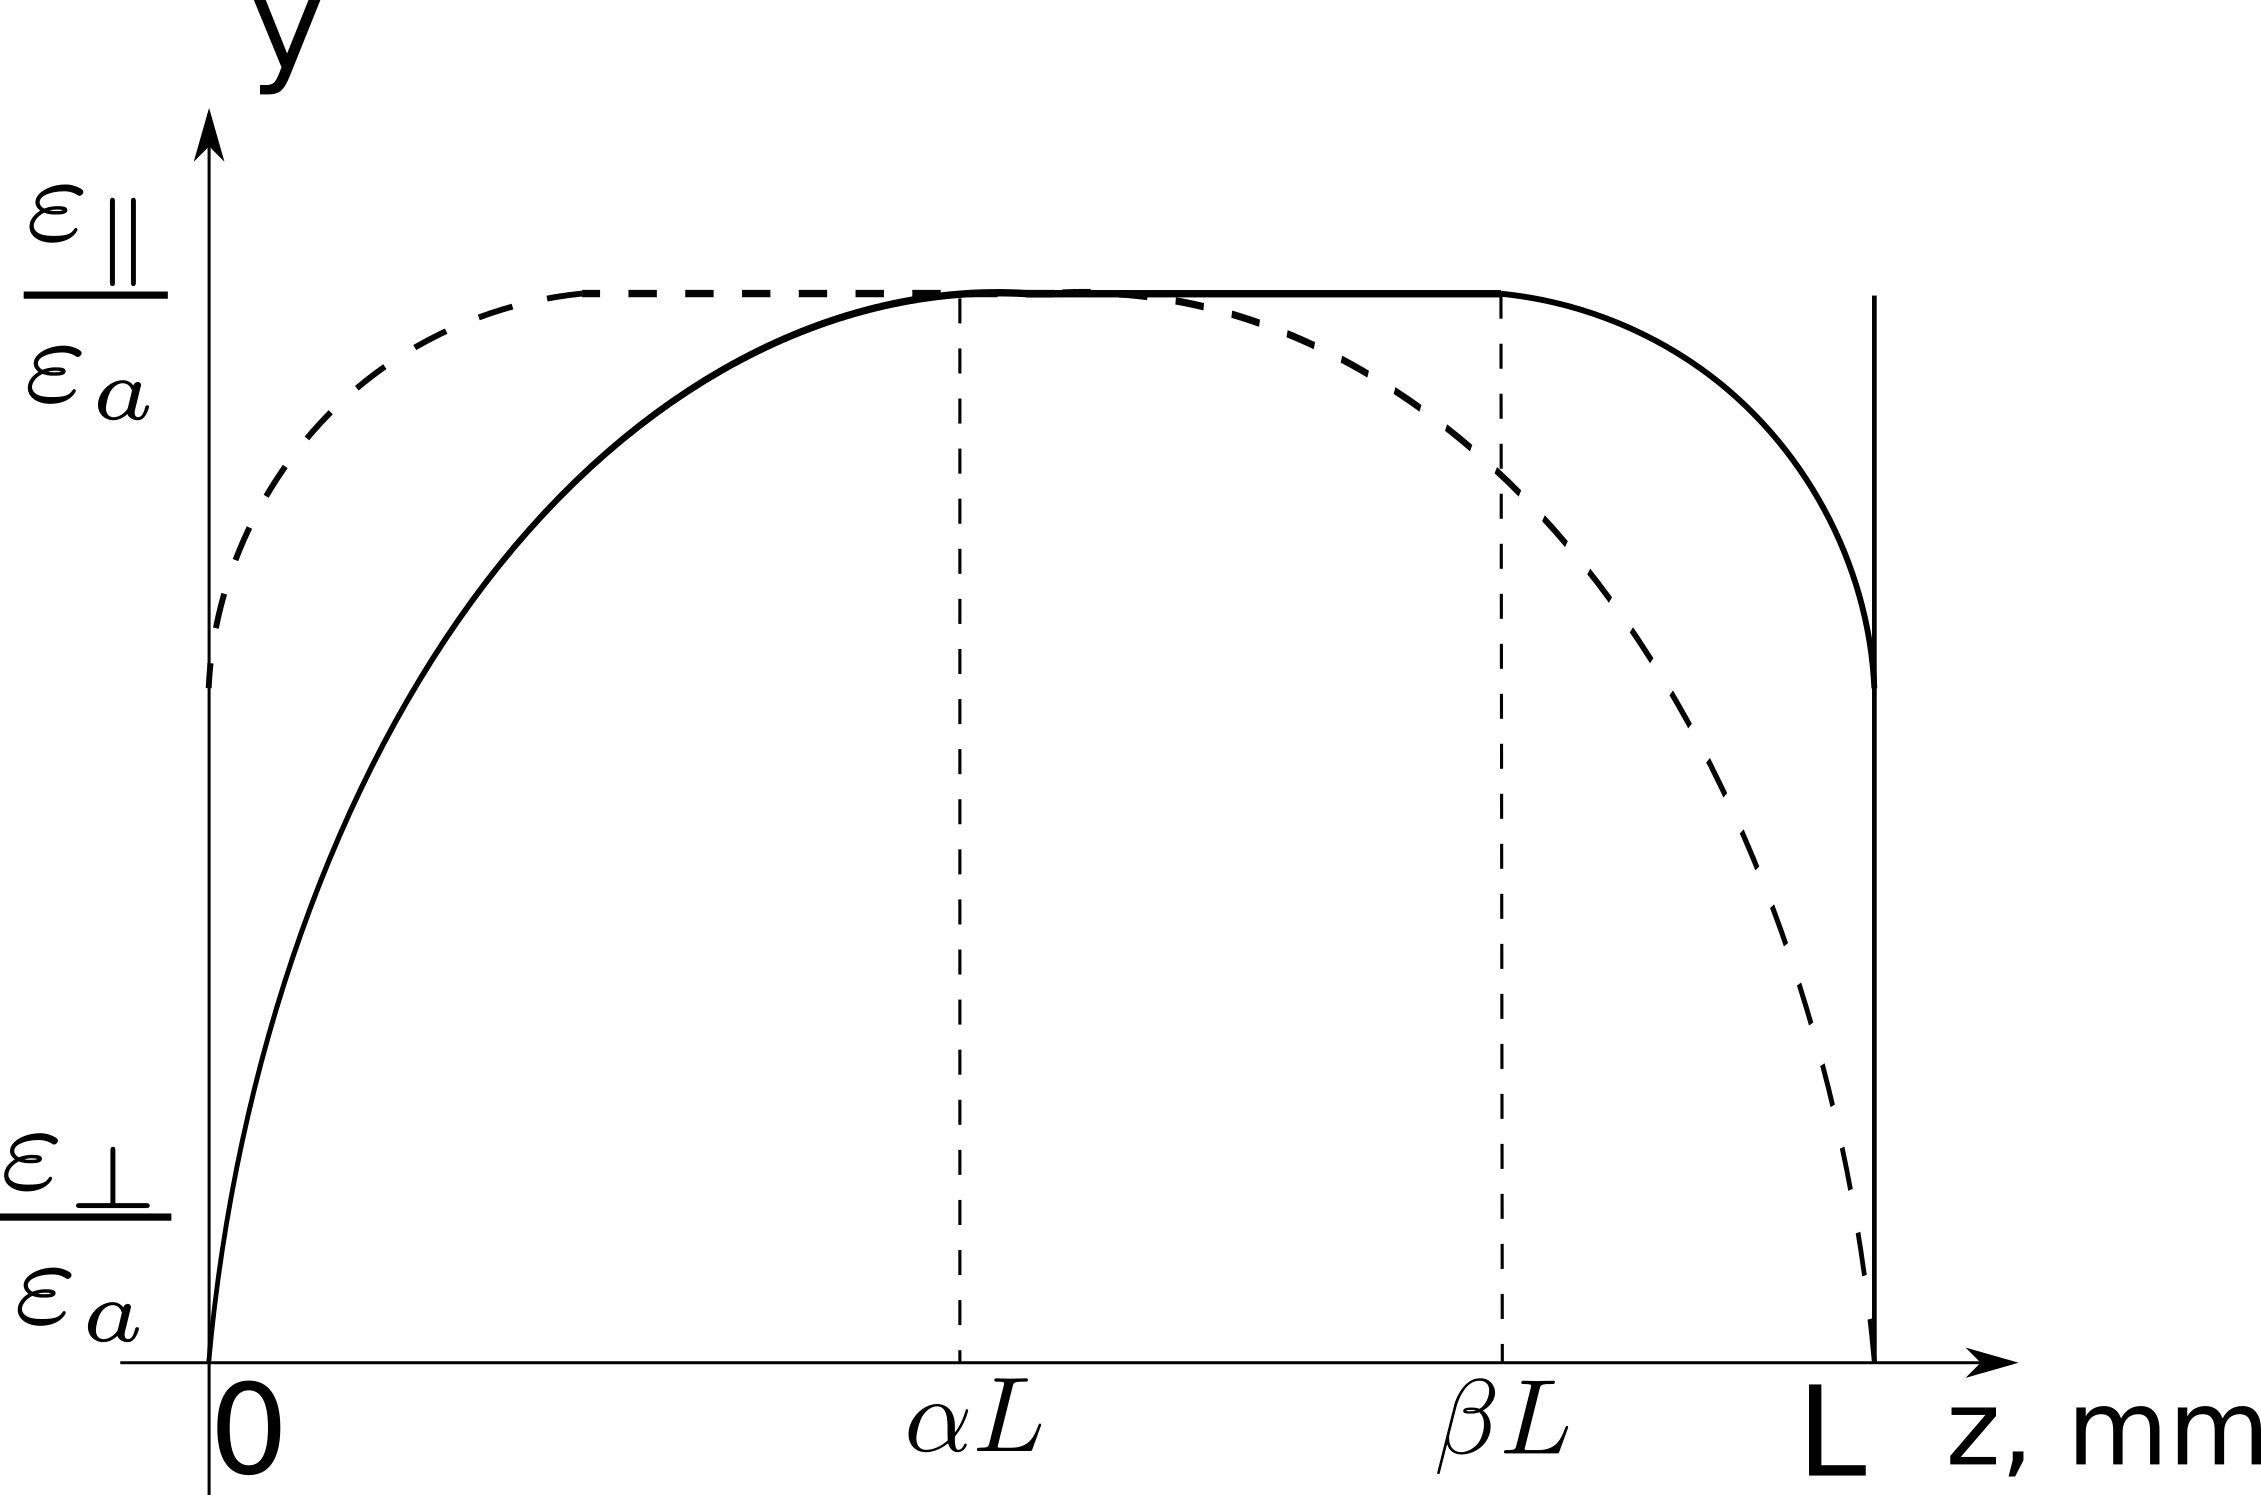
\includegraphics[width=0.9\textwidth]{Profiles_saturated_key.png}
%\caption{Рассматриваемые профили}
%\end{figure}
%\begin{equation*}
%%\footnotesize
%\scriptsize
%y(z) = \left\{
%\begin{aligned}
%&\frac{c_1}{4}(z+b_1)^2 - \frac{a^2}{c_1},&z/L\in [0;\alpha) \\
%&\frac{\varepsilon_\parallel}{\varepsilon_a},&z/L\in [\alpha;\beta]\\
%&\frac{c_2}{4}(z+b_2)^2 - \frac{a^2}{c_2},&z/L\in (\beta;1]
%\end{aligned}
%%\phantom{\right\}
%\right.
%\end{equation*}
%\end{minipage}
%\hfill
%\begin{minipage}{0.48\textwidth}
%\begin{block}{Уравнения}
%\vspace{-0.5cm}
%\begin{align}
%&y(0) = \varepsilon_\perp/\varepsilon_a \label{eqq1}\\
%&y(\alpha L) = \varepsilon_\parallel/\varepsilon_a\\
%&y(\beta L) = \varepsilon_\parallel/\varepsilon_a\\
%&y'(\alpha L) = 0\\
%&y'(\beta L) = 0 \label{eqq2}\\
%&a = J(J_1 - \frac{U}{4\pi\bar{e}})\\
%&y'(L) + a + g_2 y(L) = 0
%\end{align}
%\end{block}
%\vspace{-0.3cm}
%\begin{block}{Неравенства, гран. условия}
%\vspace{-0.5cm}
%\begin{align}
%&0 < \alpha < \beta < 1\\
%&y(L) \geq \varepsilon_\perp/\varepsilon_a\\
%&-y'(0) - a + g_1 y(0) \geq 0
%\end{align}
%\end{block}
%\end{minipage}
%\end{frame}
%

%
%
%\begin{frame}
%\frametitle{Большой $\bar{e}$ и высокое $U$}
%\framesubtitle{Пример проверки профиля}
%\begin{block}{После применения условий \eqref{eqq1} - \eqref{eqq2}}
%\begin{equation*}
%y(z) = \left\{
%\begin{aligned}
%&-\left( \frac{z/L - \alpha}{\alpha} \right)^2 + \frac{\varepsilon_\parallel}{\varepsilon_\perp},&z/L\in [0;\alpha) \\
%&\frac{\varepsilon_\parallel}{\varepsilon_a},&z/L\in [\alpha;\beta]\\
%&-\left( \frac{z/L - \beta}{\alpha} \right)^2 + \frac{\varepsilon_\parallel}{\varepsilon_\perp},&z/L\in (\beta;1]
%\end{aligned}
%%\phantom{\right\}
%\right.
%\end{equation*}
%\end{block}
%\begin{block}{Остались уравнения}
%\vspace{-0.5cm}
%\begin{align*}
%&a = J(J_1 - \frac{U}{4\pi\bar{e}})\\
%&y'(L) + a + g_2 y(L) = 0
%\end{align*}
%\end{block}
%\end{frame}
%
%\begin{frame}
%\frametitle{Большой $\bar{e}$ и высокое $U$}
%\framesubtitle{Пример проверки профиля. Итоговое уравнение.}
%\small
%\begin{equation}
%\frac{k}{x} + \ln{x} = A(U)
%\end{equation}
%\begin{minipage}{0.49\textwidth}
%\begin{figure}
%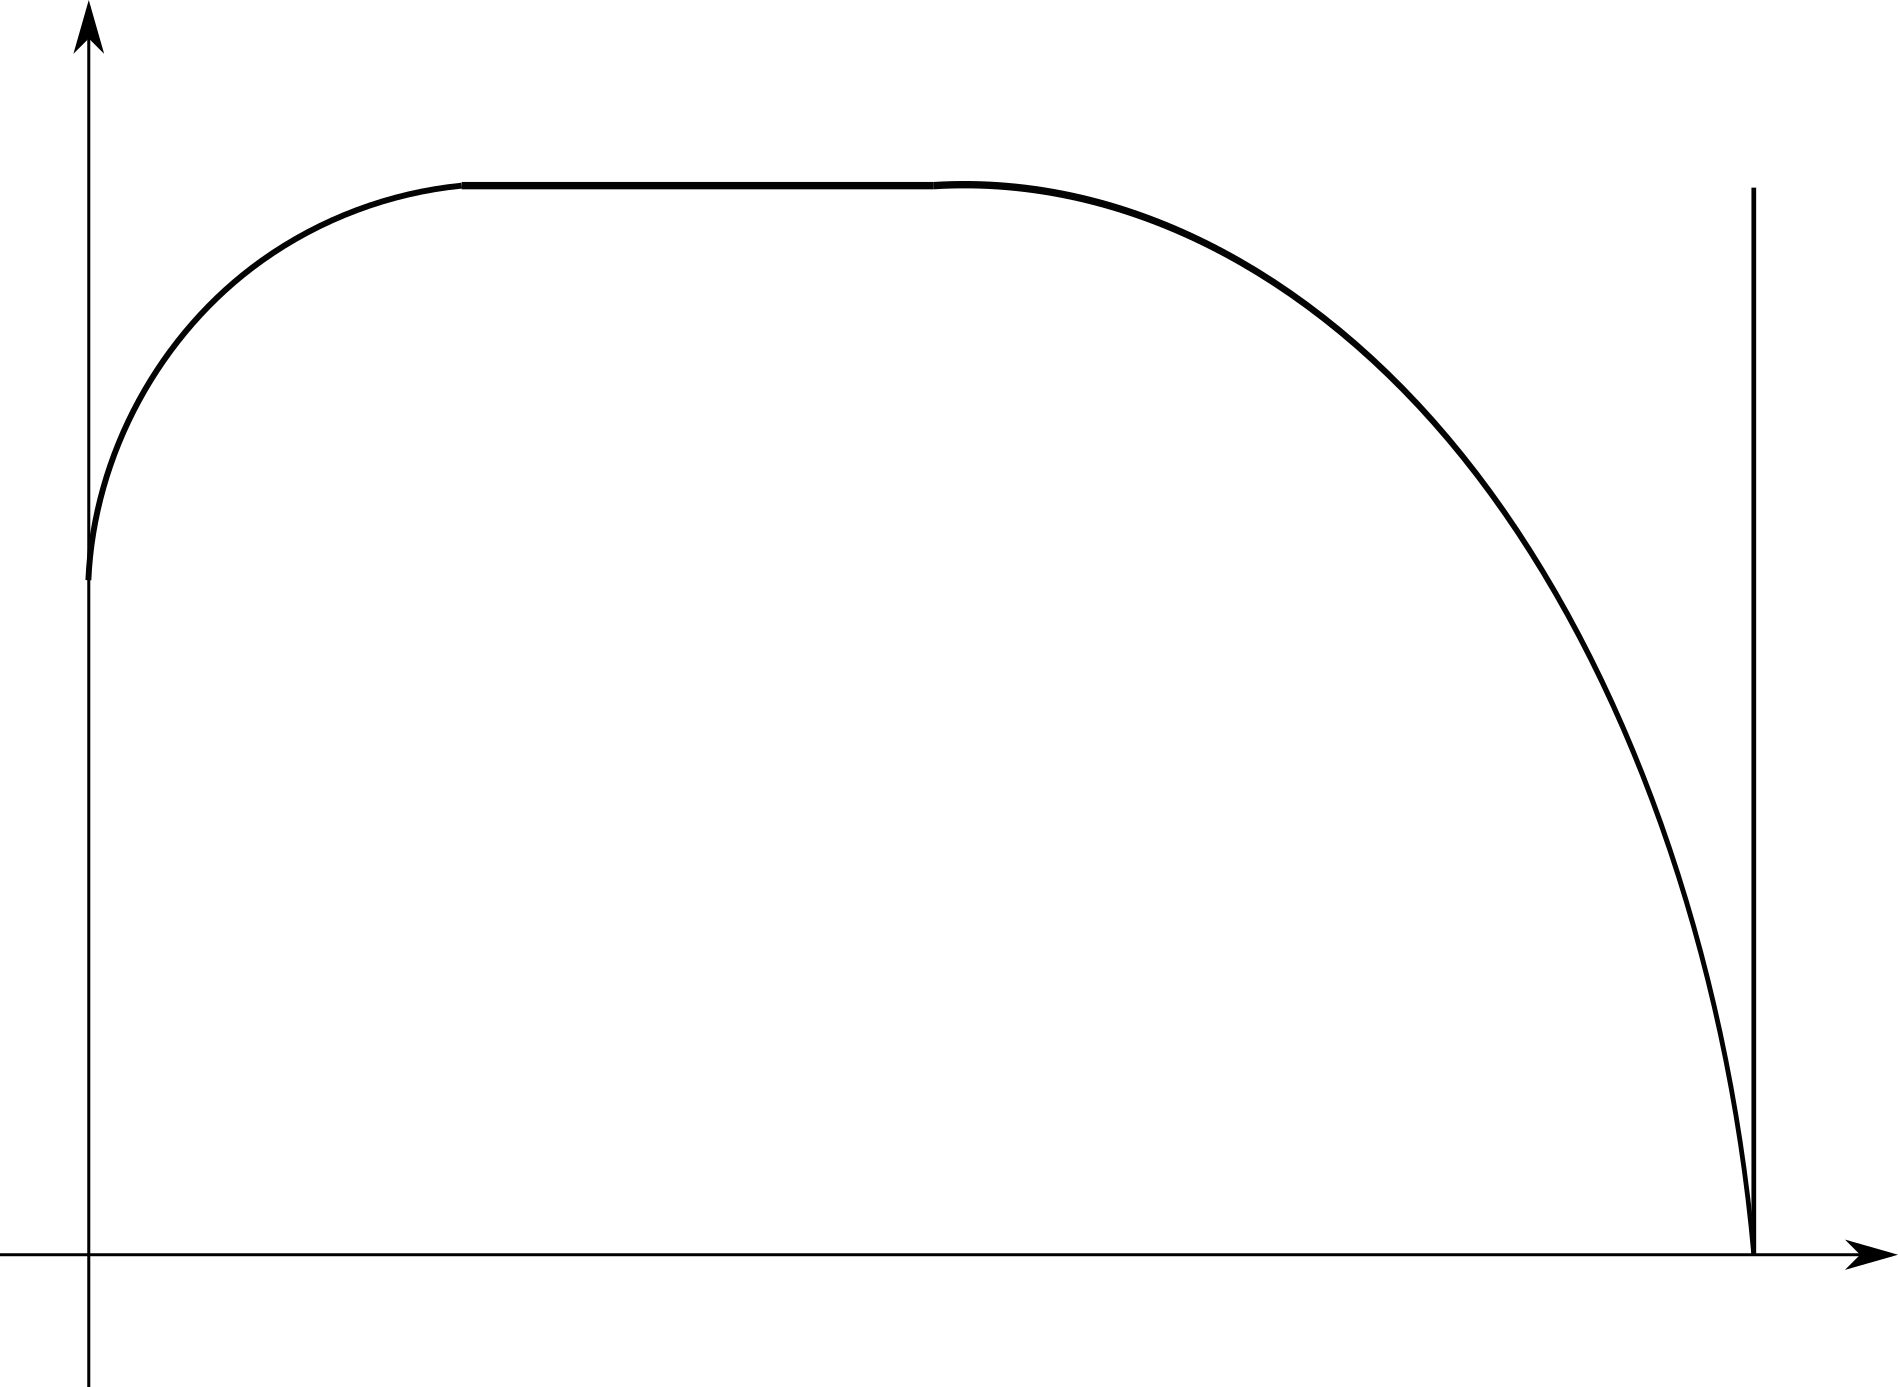
\includegraphics[width = 0.45\textwidth]{Profile_key_left.png}
%\end{figure}
%\vspace{-0.5cm}
%\begin{align*}
%&x = 1 - \beta\\
%&k = \frac{1}{\varkappa}\left( \frac{2}{g_1 L} + 1 \right)\\
%&A(U) = \frac{-\varepsilon_a U}{8\pi\bar{e}} + \frac{\varkappa + 1}{\varkappa} + \ln{\frac{k\varkappa - 1}{\varkappa + 1}}
%\end{align*}
%\end{minipage}
%\hfill
%\begin{minipage}{0.49\textwidth}
%\begin{figure}
%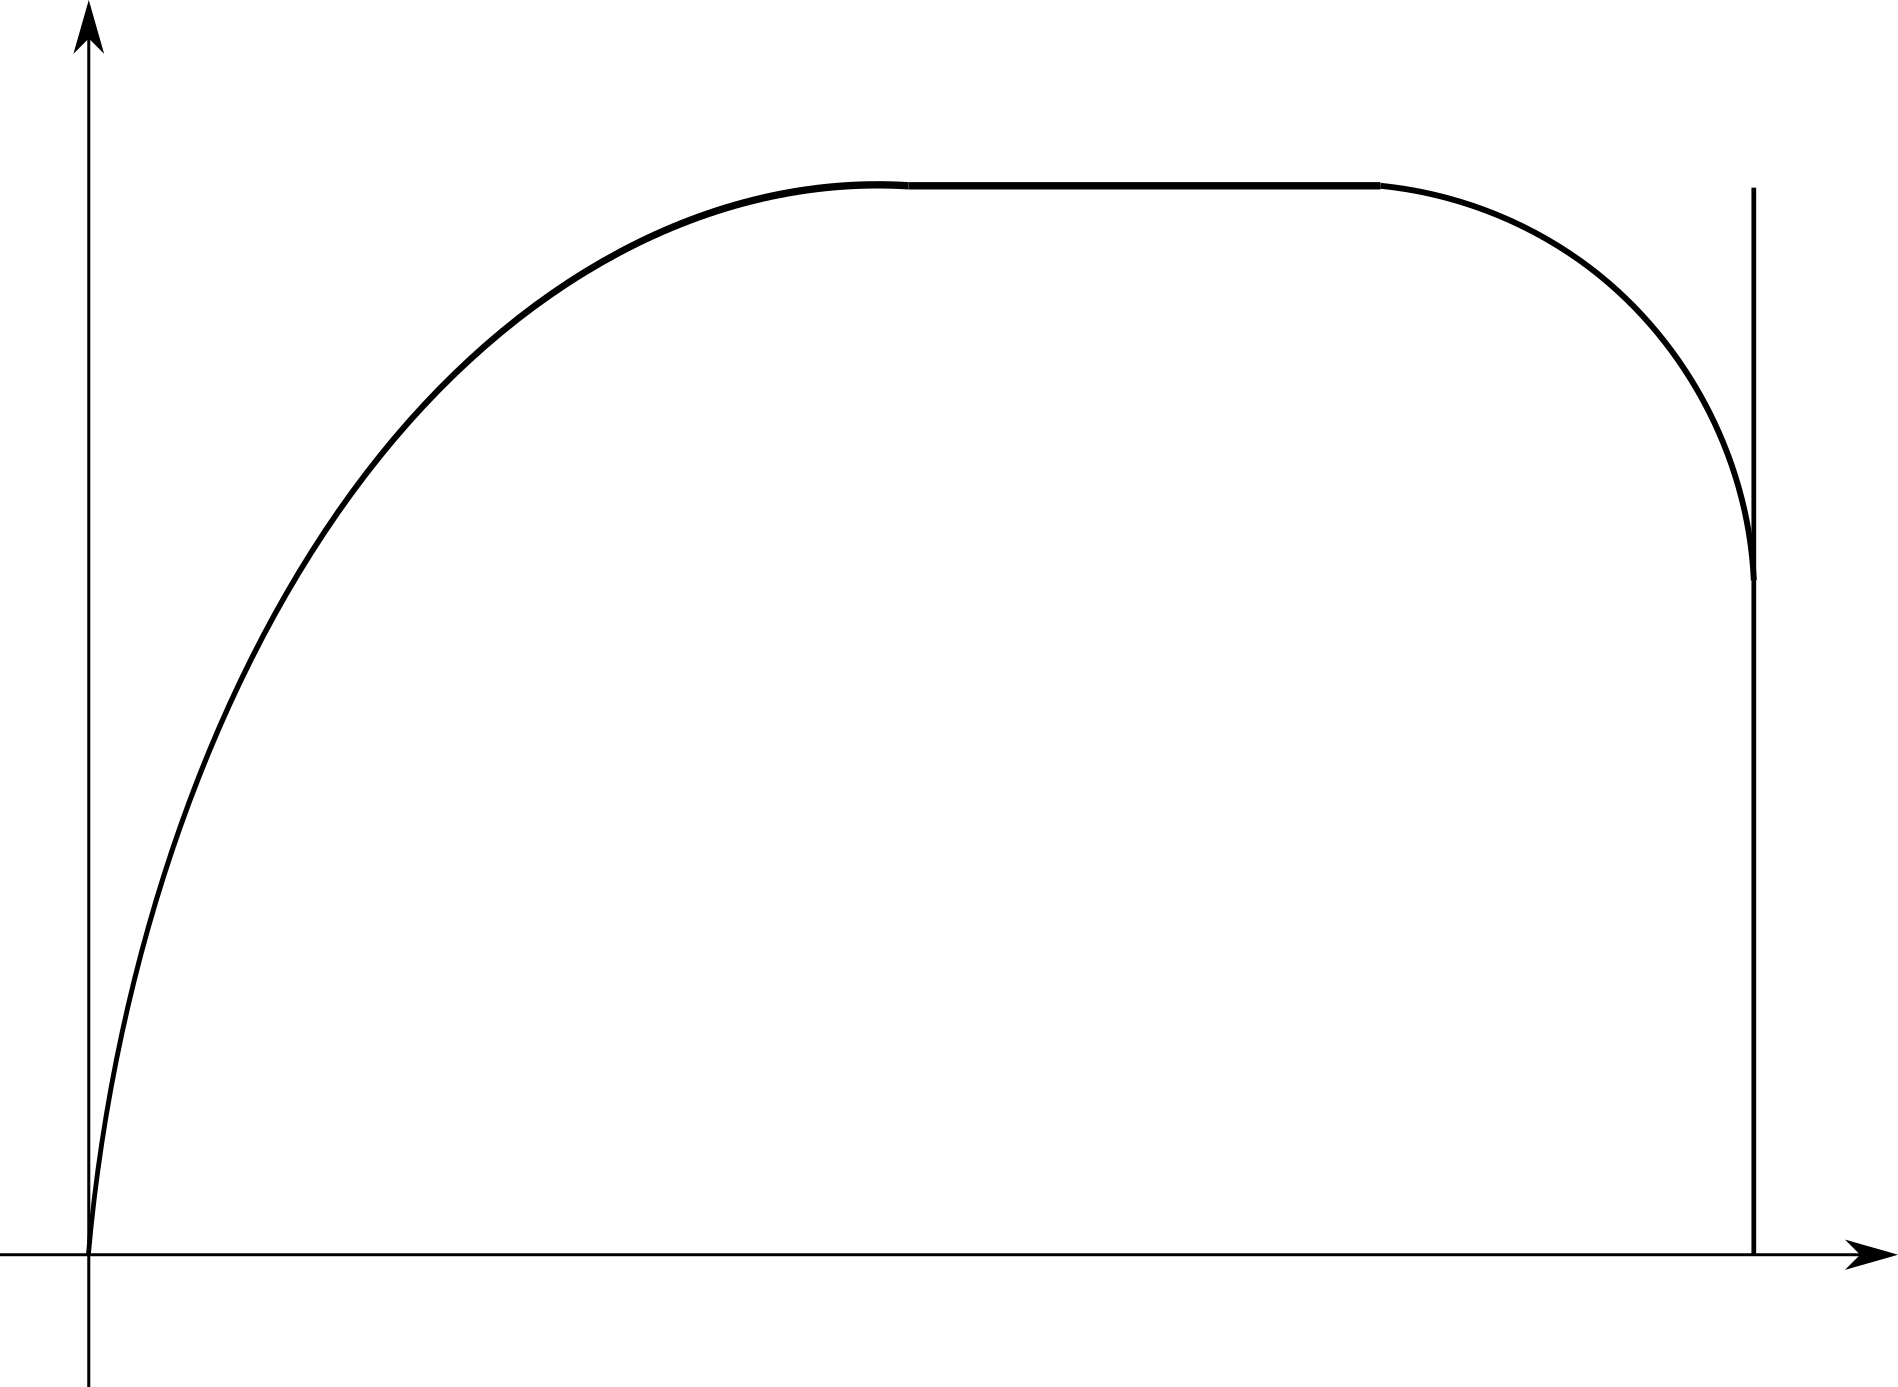
\includegraphics[width = 0.45\textwidth]{Profile_key_right.png}
%\end{figure}
%\vspace{-0.5cm}
%\begin{align*}
%&x = \alpha\\
%&k = \frac{1}{\varkappa}\left( \frac{2}{g_2 L} + 1 \right)\\
%&A(U) = \frac{\varepsilon_a U}{8\pi\bar{e}} + \frac{\varkappa + 1}{\varkappa} + \ln{\frac{k\varkappa - 1}{\varkappa + 1}}
%\end{align*}
%\end{minipage}
%%\begin{block}{Результат}
%%123
%%\end{block}
%\end{frame}
%
%\begin{frame}
%\frametitle{Большой $\bar{e}$ и высокое $U$}
%\framesubtitle{График уравнения}
%%\begin{block}{456}
%\begin{figure}
%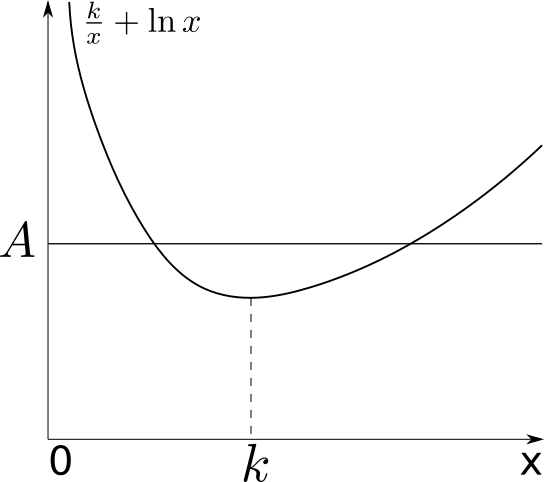
\includegraphics[width = 0.5\textwidth]{Plot_F(x).png}
%\caption{Общий вид графика функции $\frac{k}{x} + \ln{x}$}
%\end{figure}
%%\end{block}
%\end{frame}
%
%\begin{frame}
%\frametitle{Большой $\bar{e}$ и высокое $U$}
%\framesubtitle{ОДЗ переменной $x$}
%\begin{figure}
%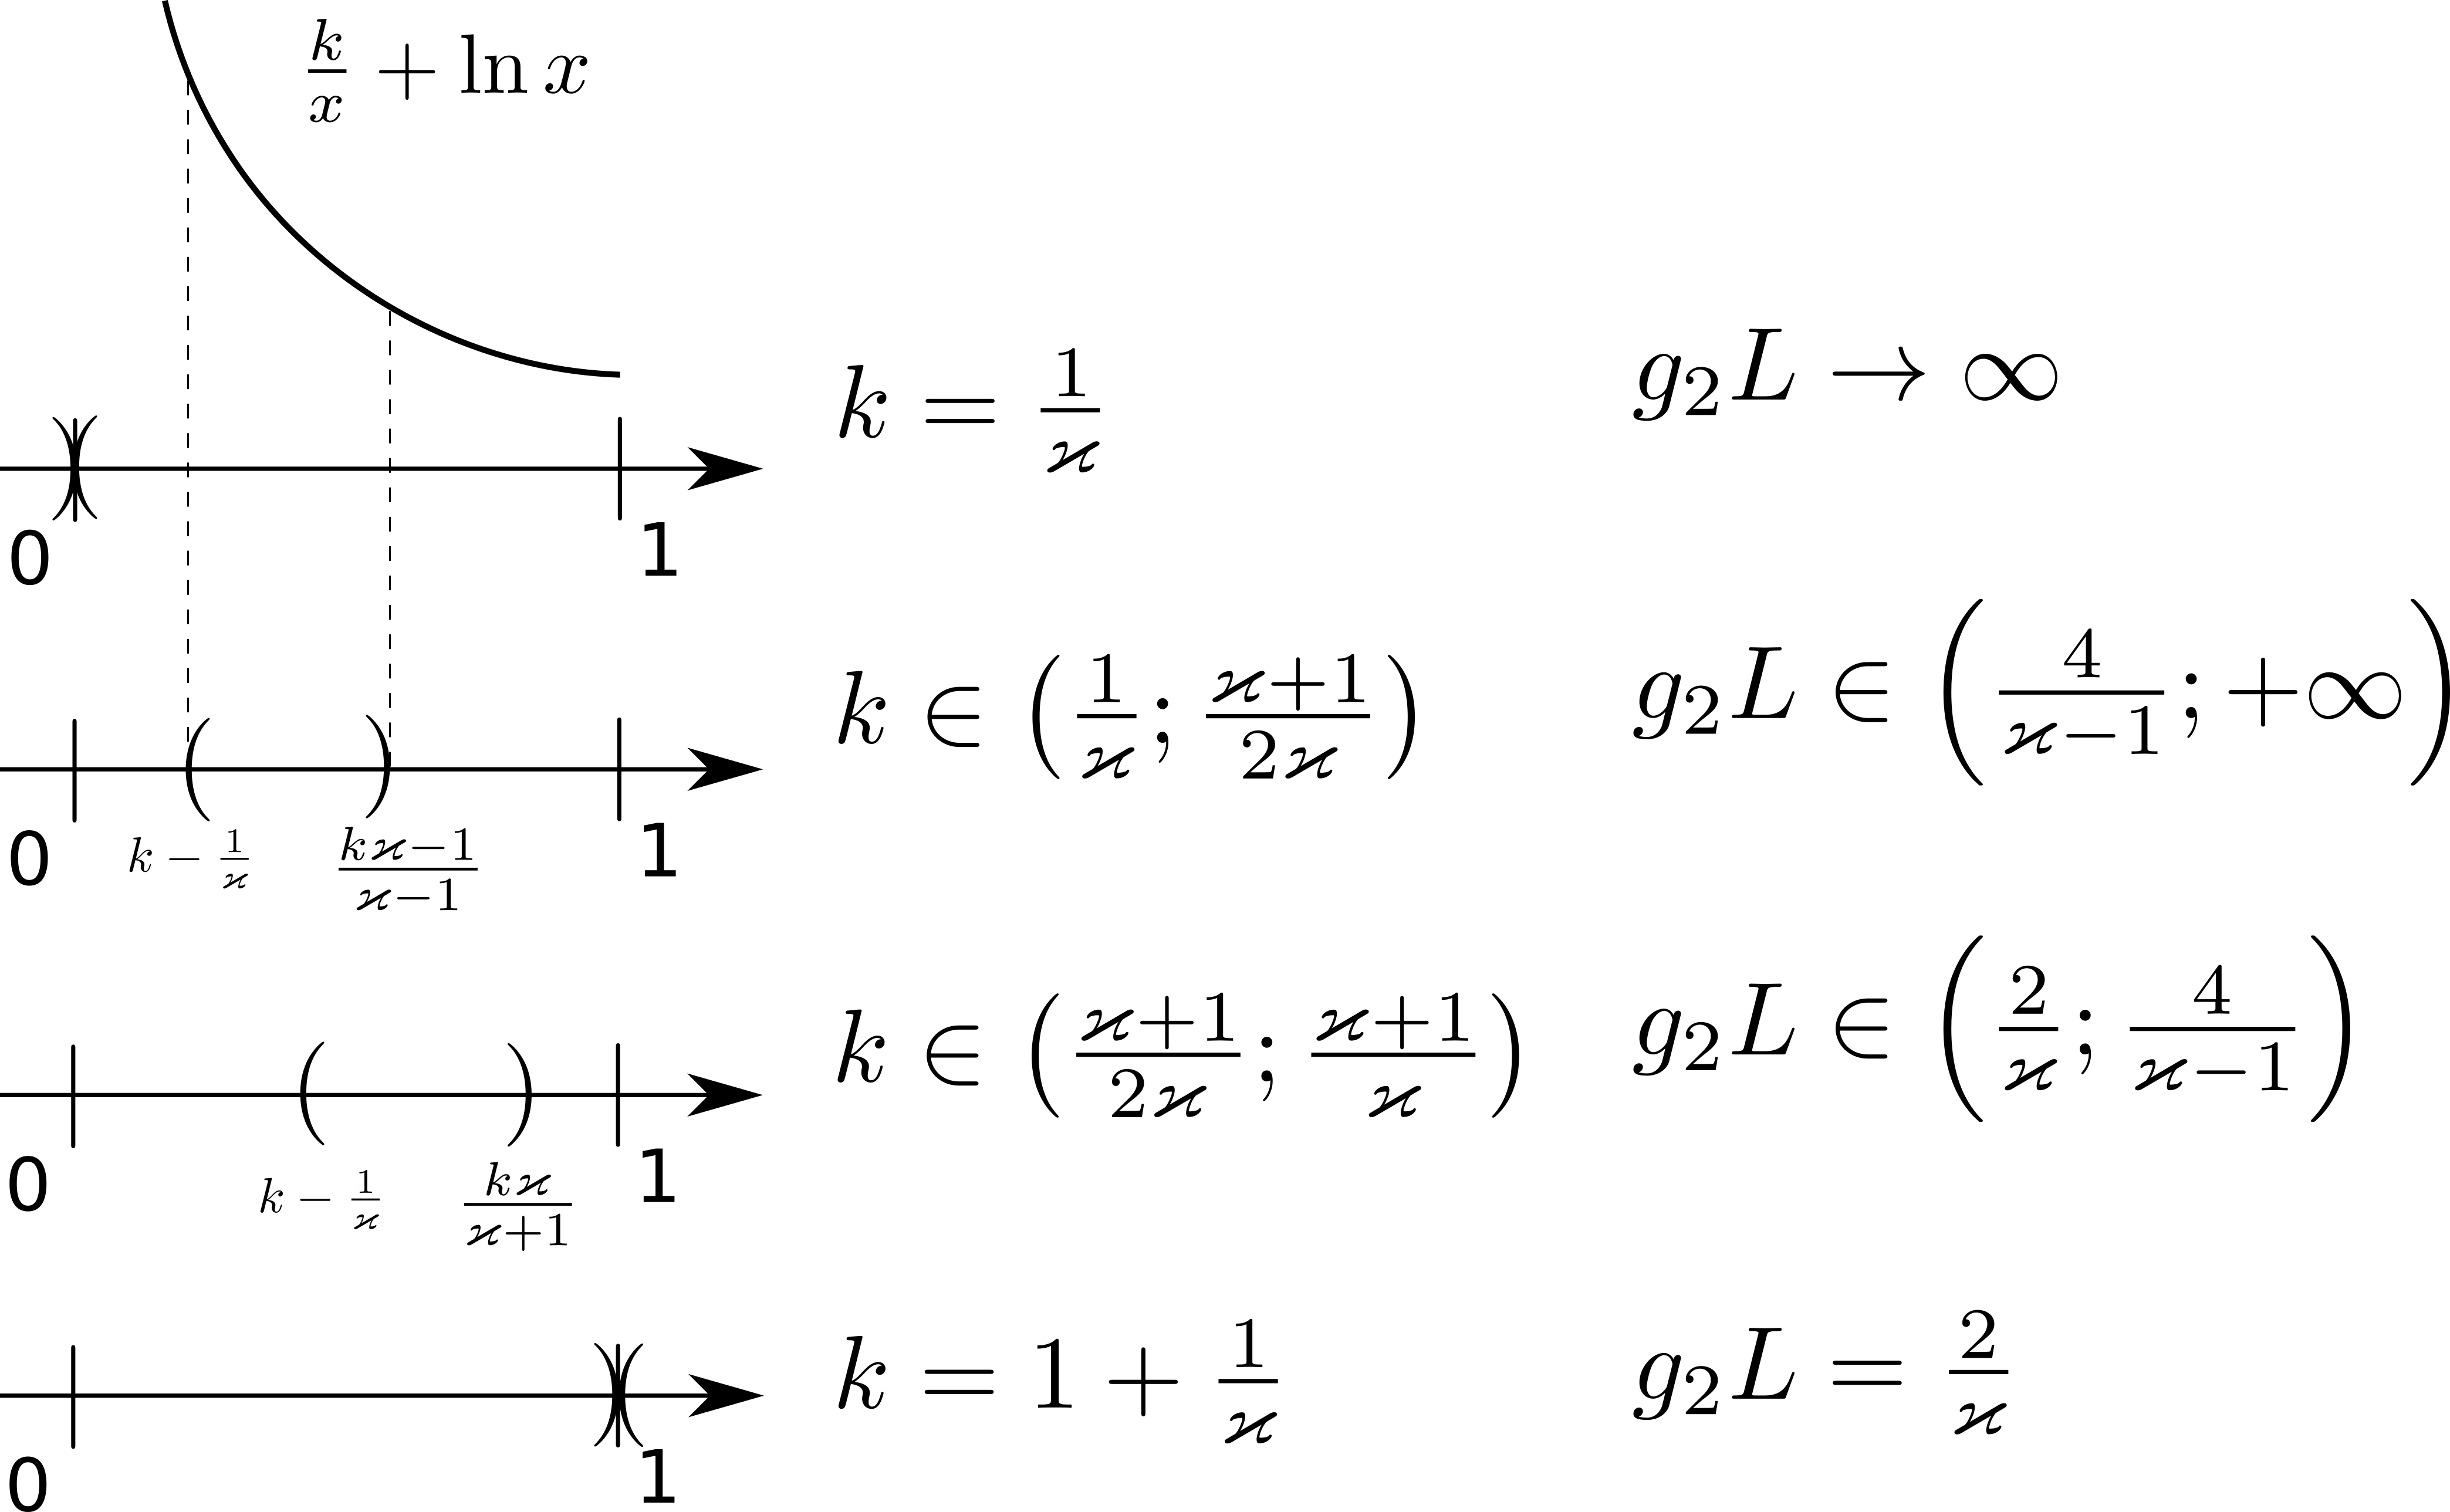
\includegraphics[width = \textwidth]{Inequalities_k.png}
%\end{figure}
%\end{frame}

\begin{frame}
\frametitle{Большой $\bar{e}$ и высокое $U$}
\framesubtitle{Схема переходов}
%\begin{block}{456}
%123
%\end{block}
\begin{figure}
\includegraphics[width = \textwidth]{Scheme.png}
\caption{Схема трансформаций ориентационной структуры}
\end{figure}
\end{frame}





\begin{frame}
\frametitle{Большой $\bar{e}$ и высокое $U$}
\framesubtitle{Справка}
\begin{block}{Выражения для характеристических напряжений}
\begin{align}
&\widetilde{U} = \frac{8\pi\bar{e}}{\varepsilon_a} \ln{\left( 1 + \frac{g_2 L}{2} \right)} \\
&\hat{U}_1 = \frac{8\pi\bar{e}}{\varepsilon_a} \ln{\left(\frac{\varkappa+1}{\varkappa} \right)}\\
&\hat{U}_2 = \frac{8\pi\bar{e}}{\varepsilon_a} \left[\frac{g_2 L}{2} - \frac{1}{\varkappa} + \ln{\left(\frac{\varkappa+1}{\varkappa} \right)} \right]\\
&\hat{U}' = \frac{8\pi\bar{e}}{\varepsilon_a} \ln{\left(\frac{\varkappa+1}{\varkappa - 1} \right)}\\
&\widetilde{U}' = \frac{8\pi\bar{e}}{\varepsilon_a} \left[\frac{g_2 L}{2}\frac{\varkappa - 1}{\varkappa} - \frac{2}{\varkappa} + \ln{\left(\frac{\varkappa+1}{\varkappa - 1} \right)} \right]
\end{align}
\end{block}
\end{frame}

\begin{frame}
\frametitle{Большой $\bar{e}$ и высокое $U$}
\framesubtitle{Профили при слабом зацеплении}
\begin{figure}[h]
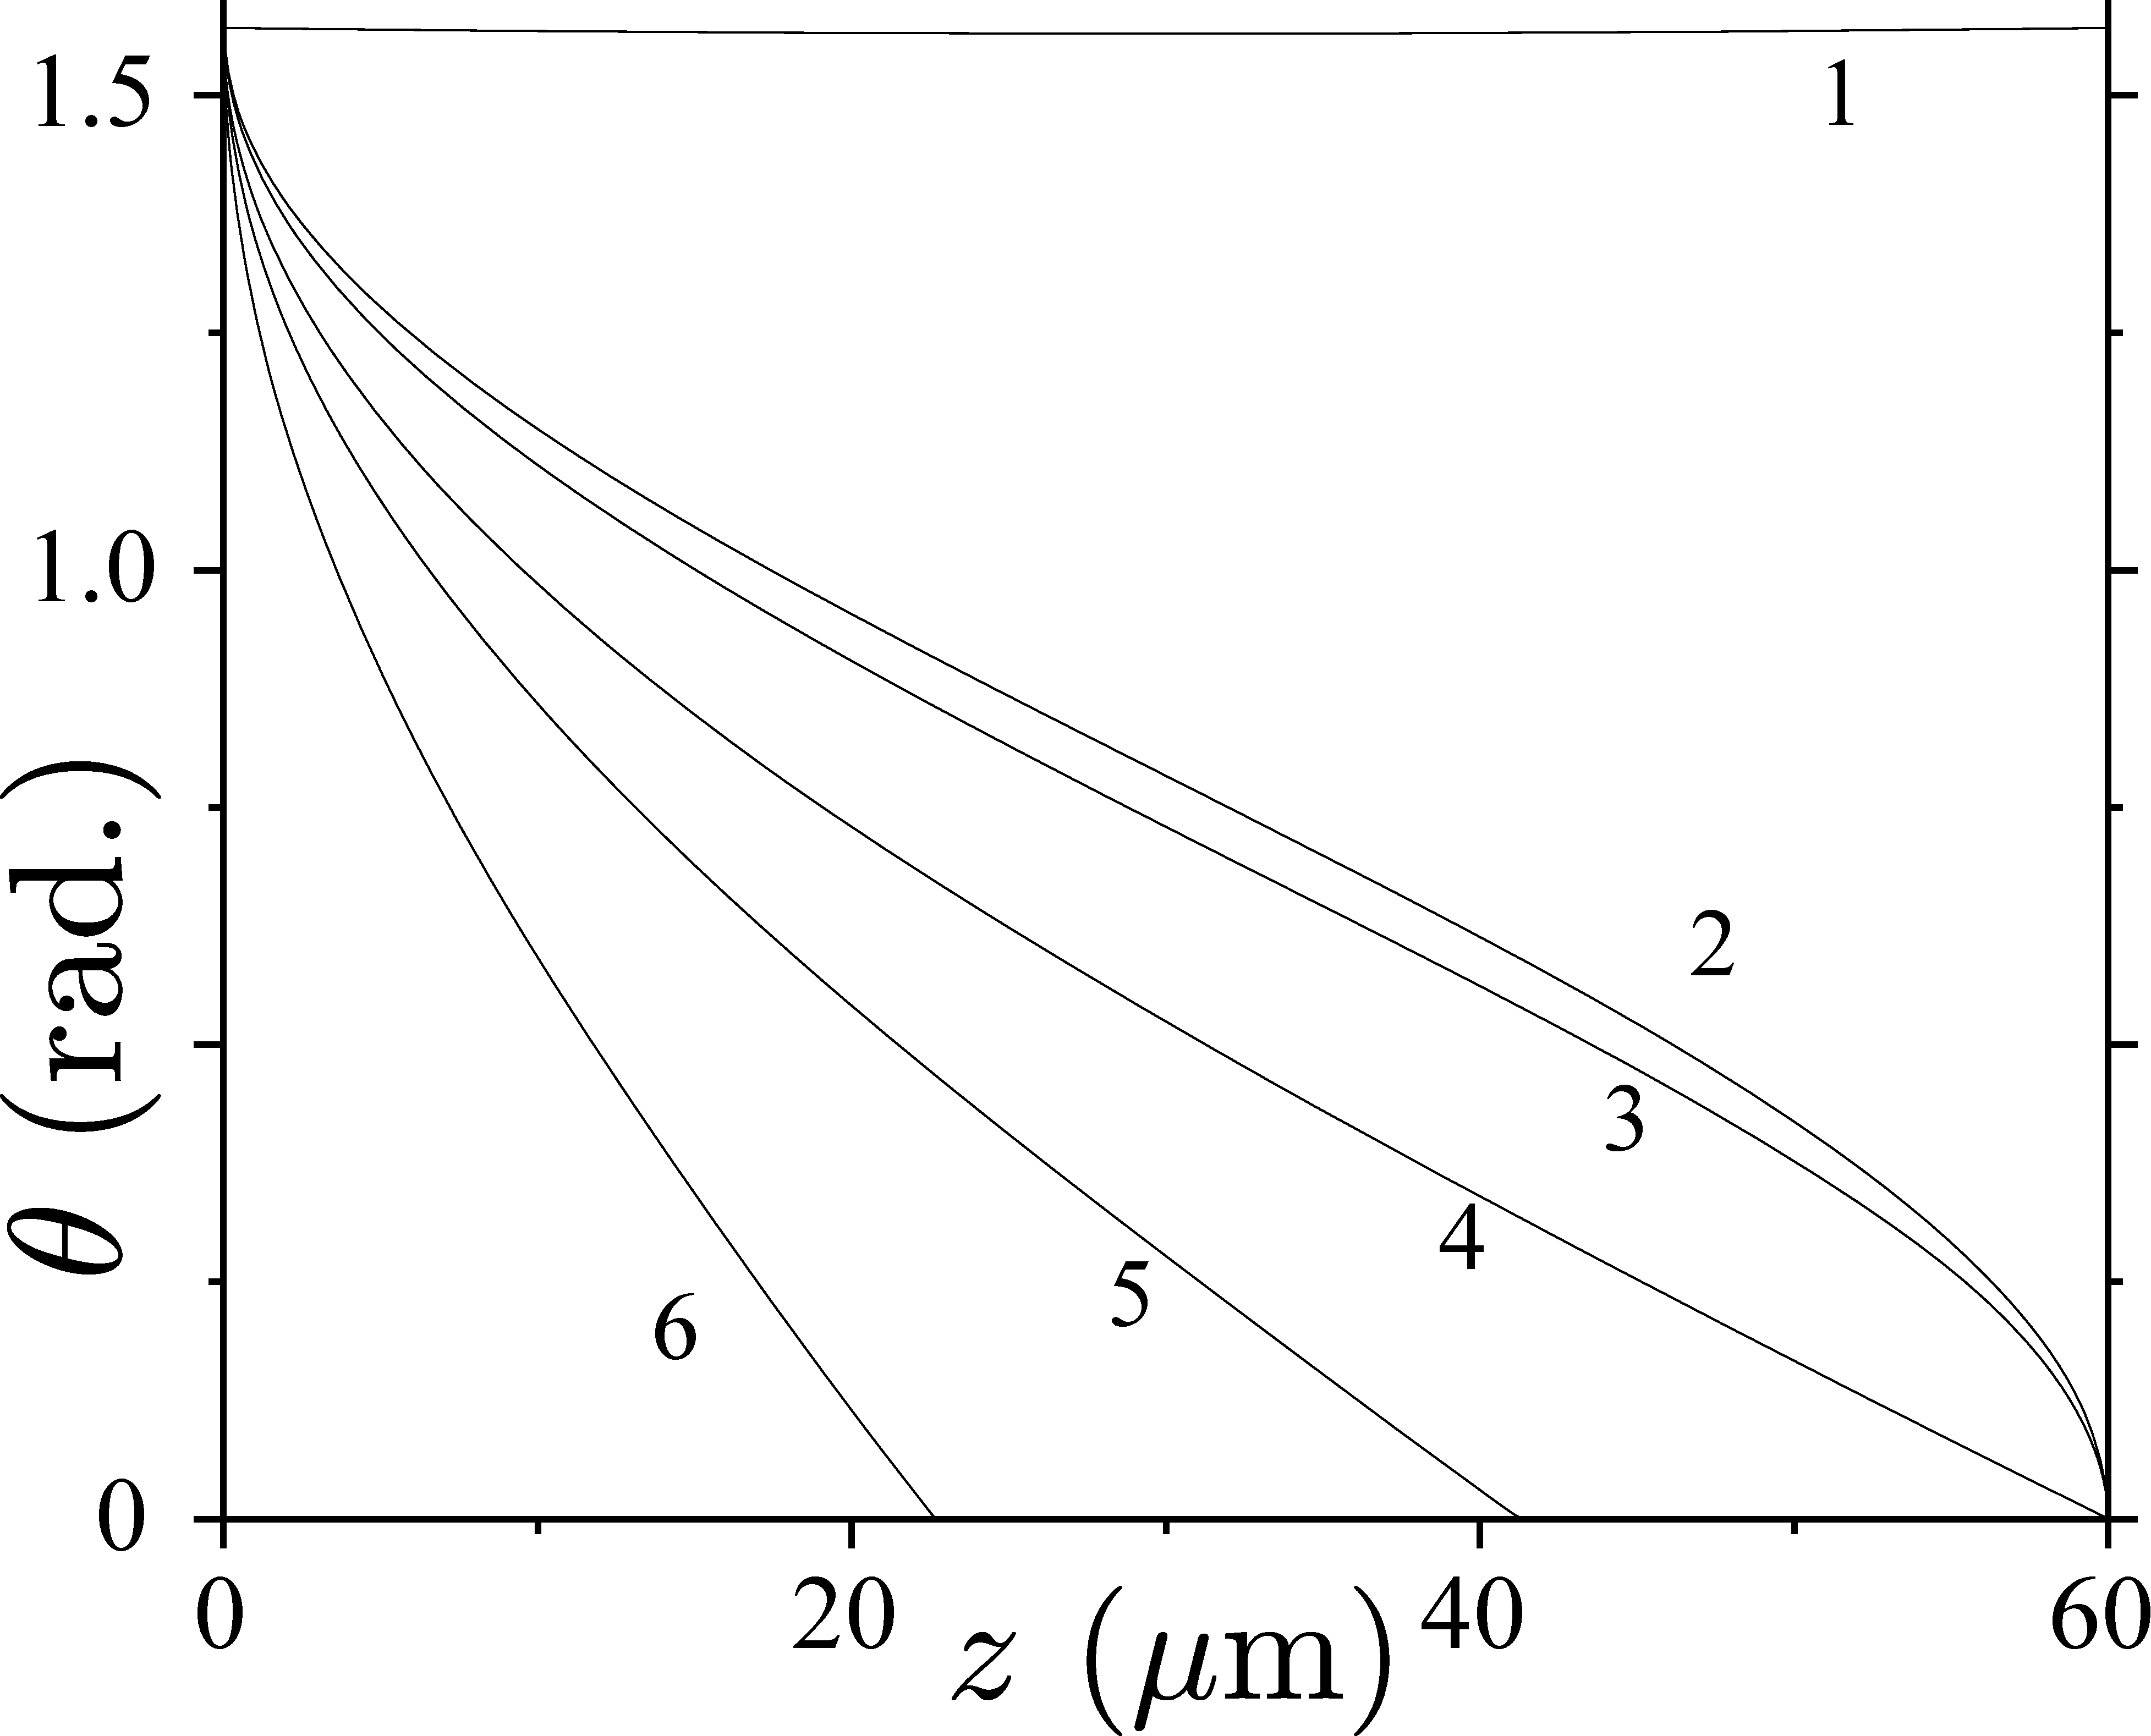
\includegraphics[width=0.45\textwidth]{Fig1_theta_low_anchoring.eps}%\hspace{2pc}%
\hfill
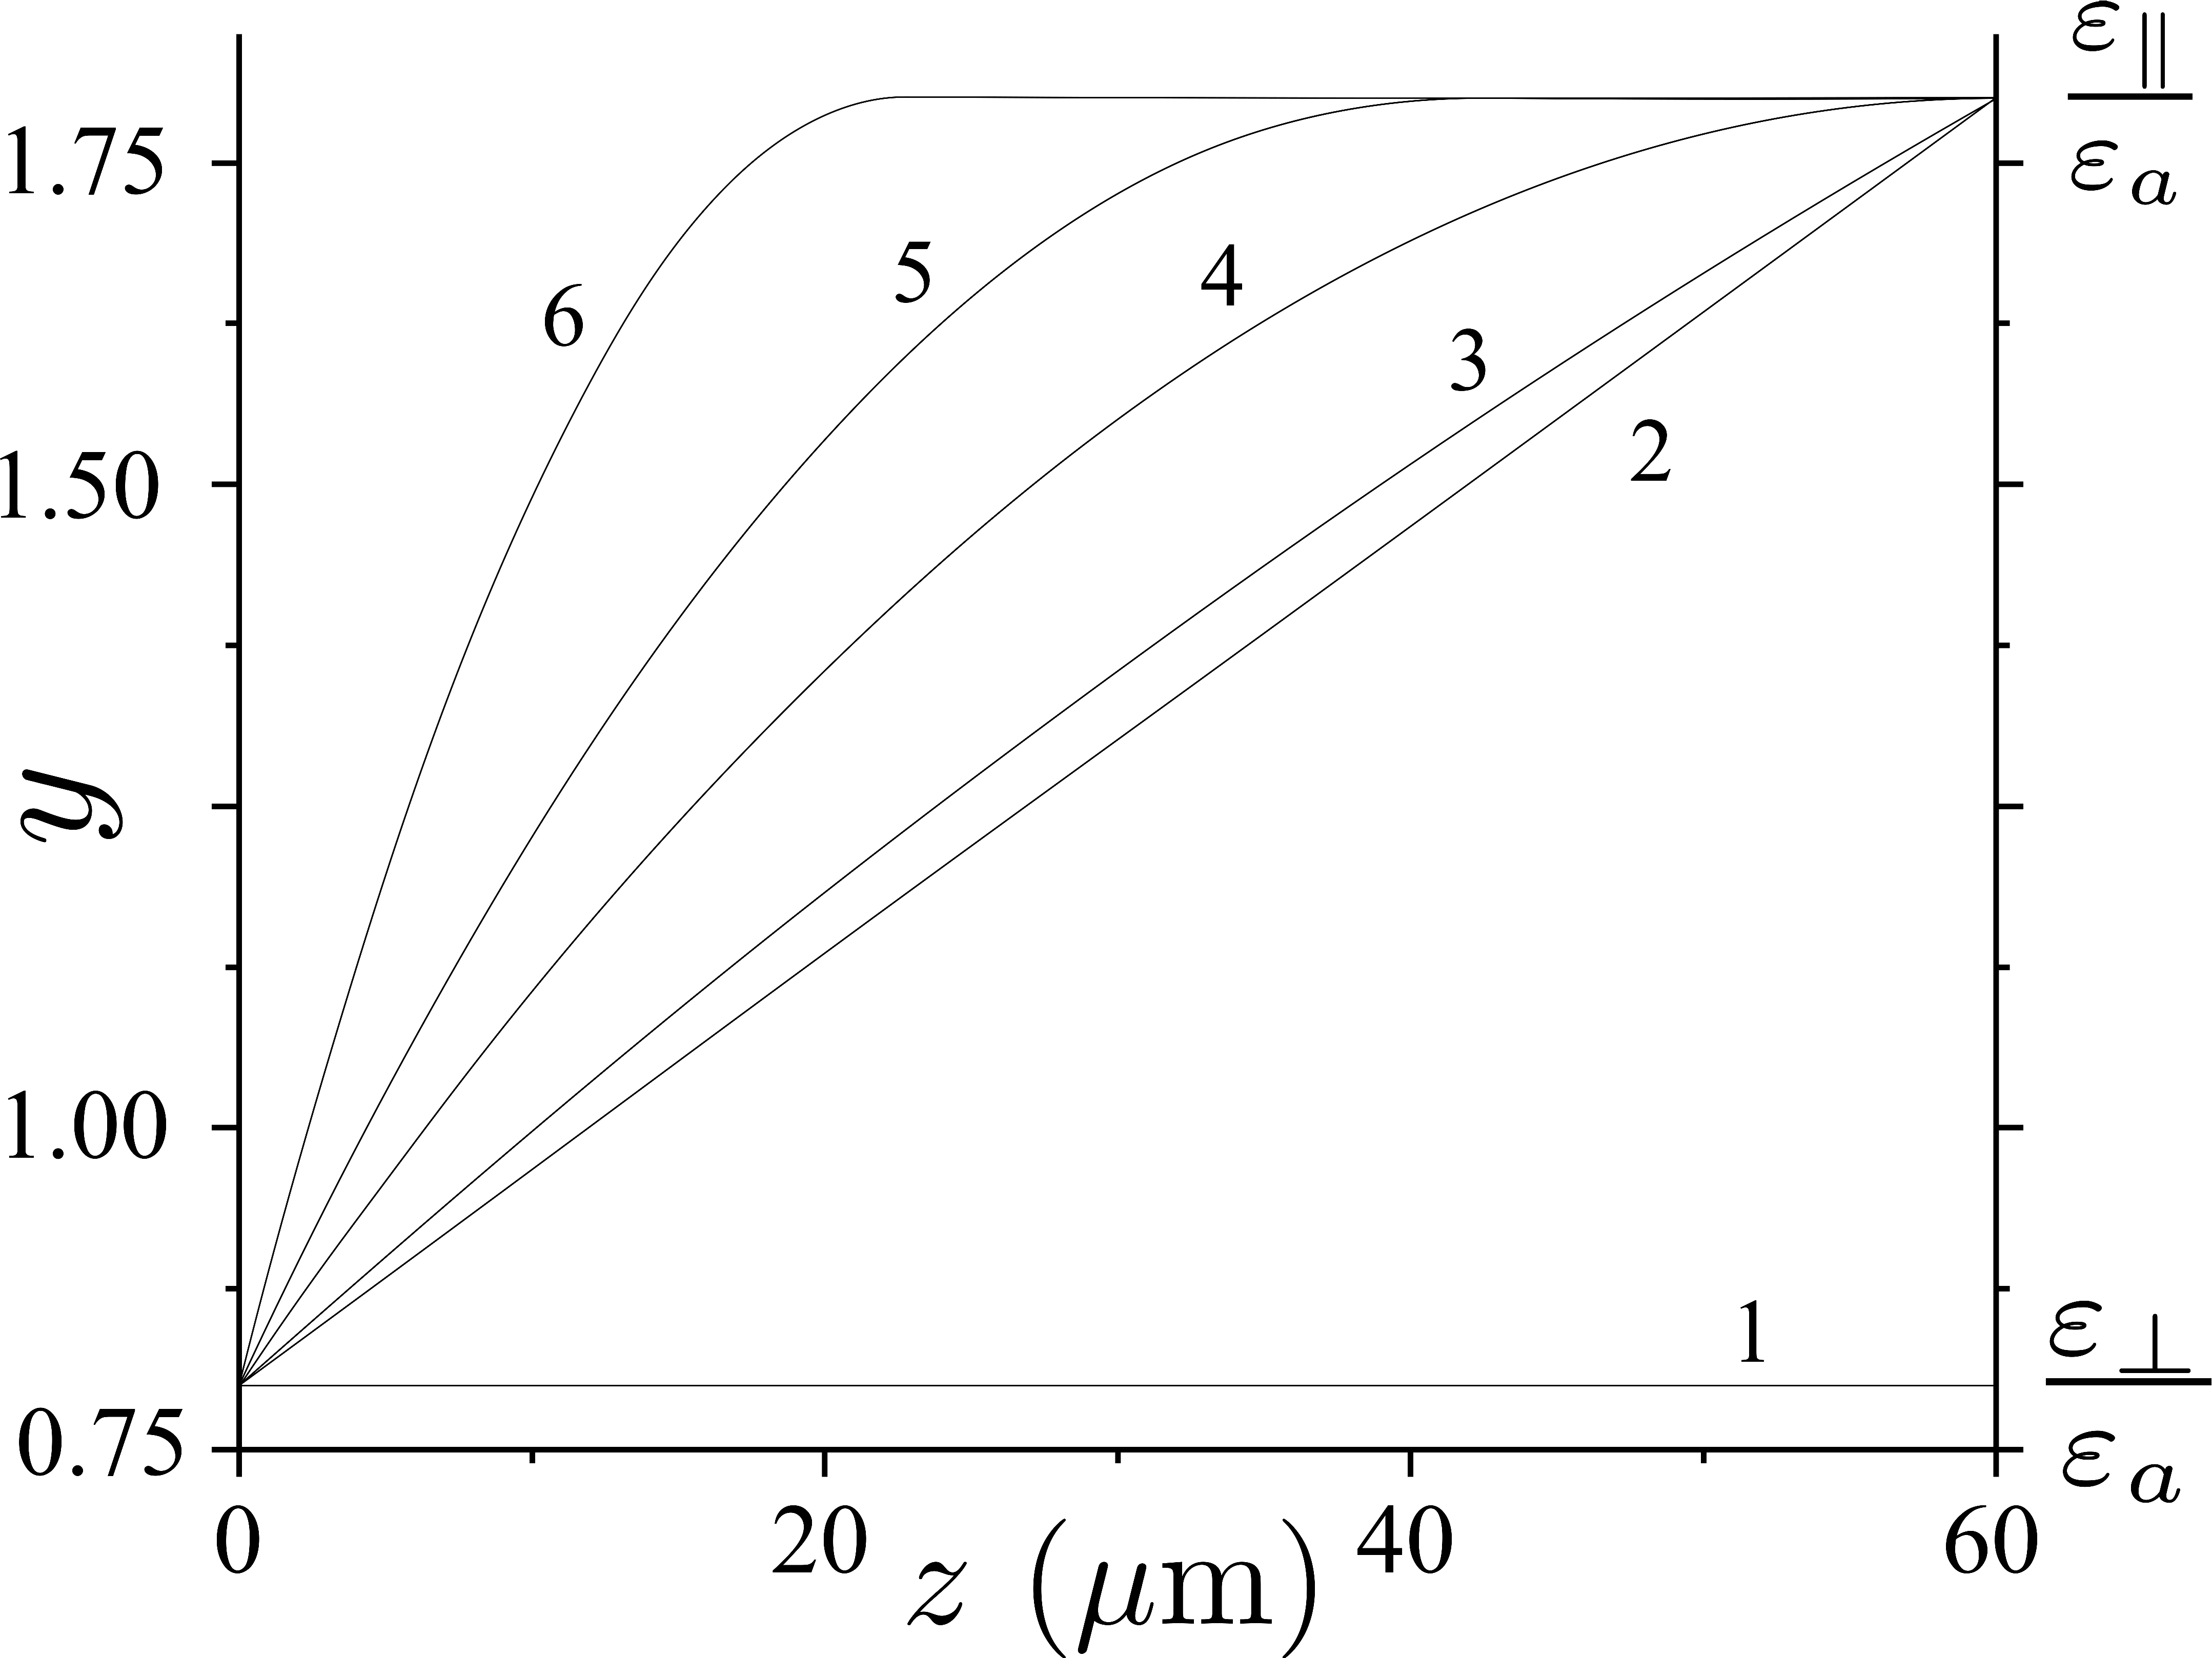
\includegraphics[width = 0.49\textwidth]{Fig1_y_low_anchoring.eps}
\caption{\footnotesize Профили $\theta(z)$ (слева) и зависимости $y(z)$ (справа), полученные для случая слабого зацепления, когда выполнено $g_2 L < 2/\varkappa$. Модули поверхностного зацепления: $W_\theta^{(1)}=0.0025\ \mathrm{erg}/\mathrm{cm}^2$, $W_\theta^{(2)} = 5\times 10^{-4}\ \mathrm{erg}/\mathrm{cm}^2$ для всех кривых. Приложенное напряжение в соответствии с линиями: 1 -- $U = 0.04\,\mathrm{V}$, 2 -- $U = 0.05\,\mathrm{V}$, 3 -- $U = 1.5\,\mathrm{V}$, 4 -- $U = 4.67\,\mathrm{V}$, 5 -- $U = 7.5\,\mathrm{V}$, 6 -- $U = 15\,\mathrm{V}$.}
\end{figure}
\end{frame}


\begin{frame}
\frametitle{Большой $\bar{e}$ и высокое $U$}
\framesubtitle{Профили при среднем зацеплении}
\begin{figure}[h]
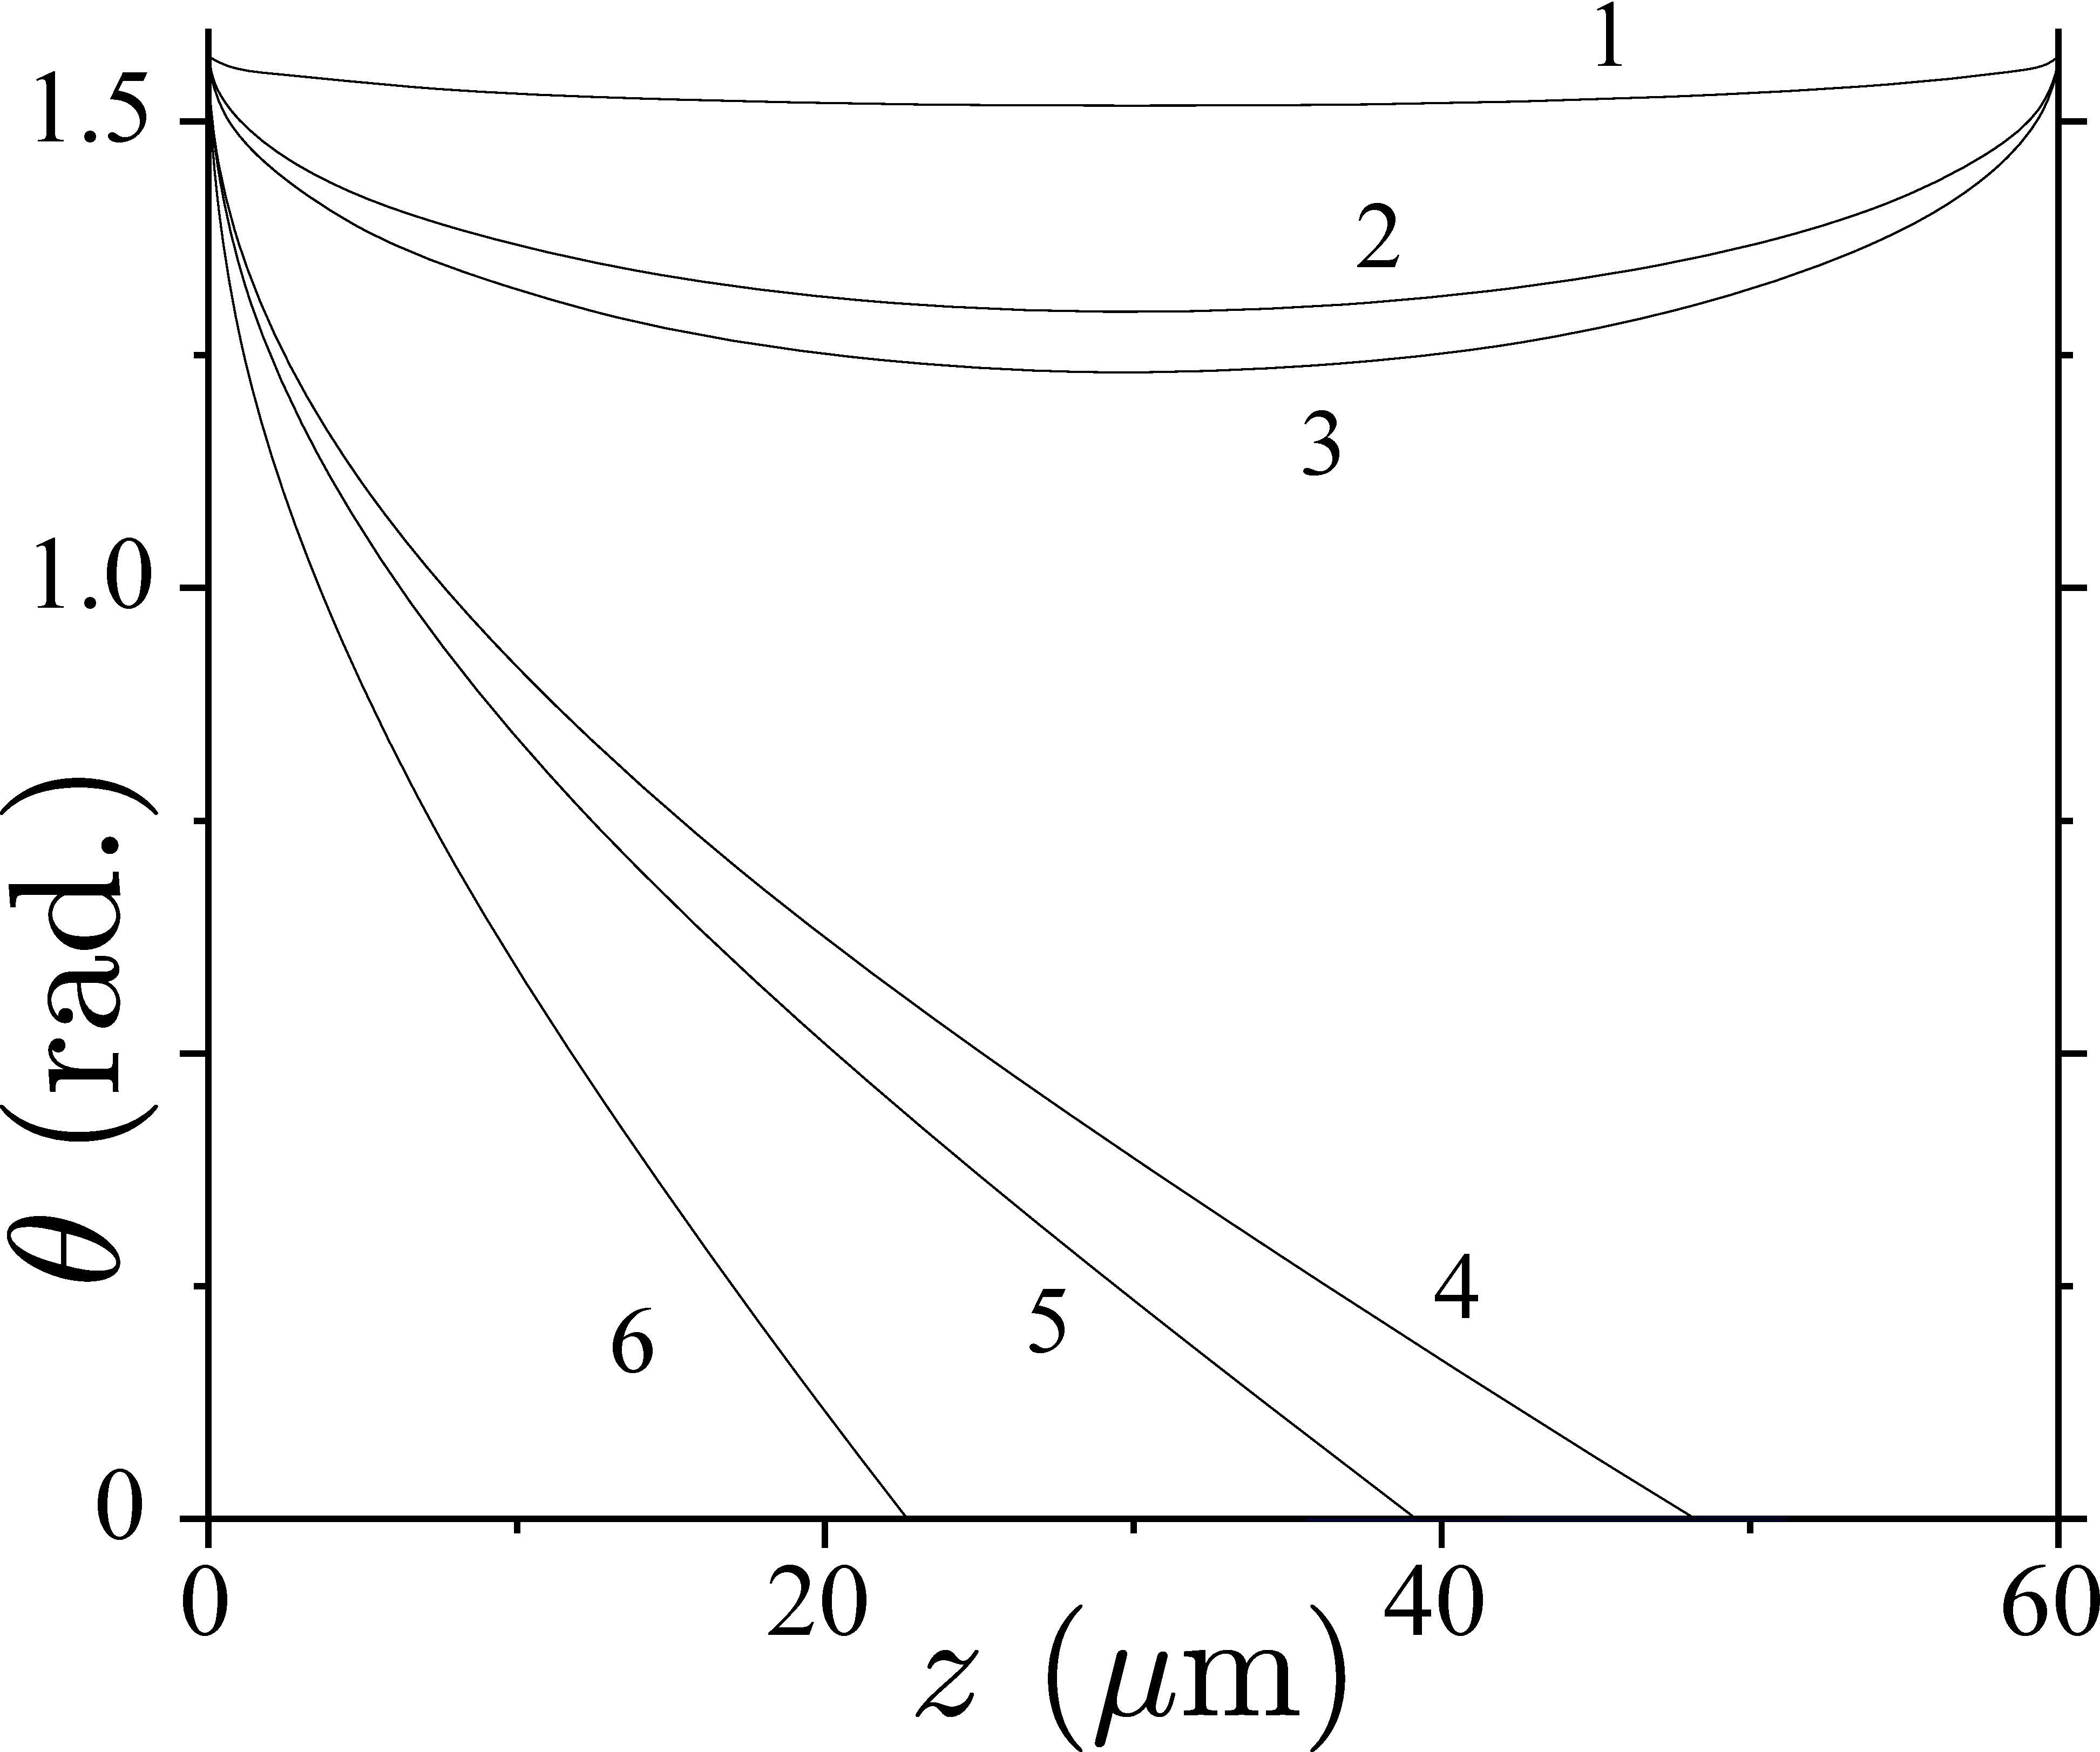
\includegraphics[width=0.45\textwidth]{Fig2_theta_mid_anchoring.eps}%\hspace{2pc}%
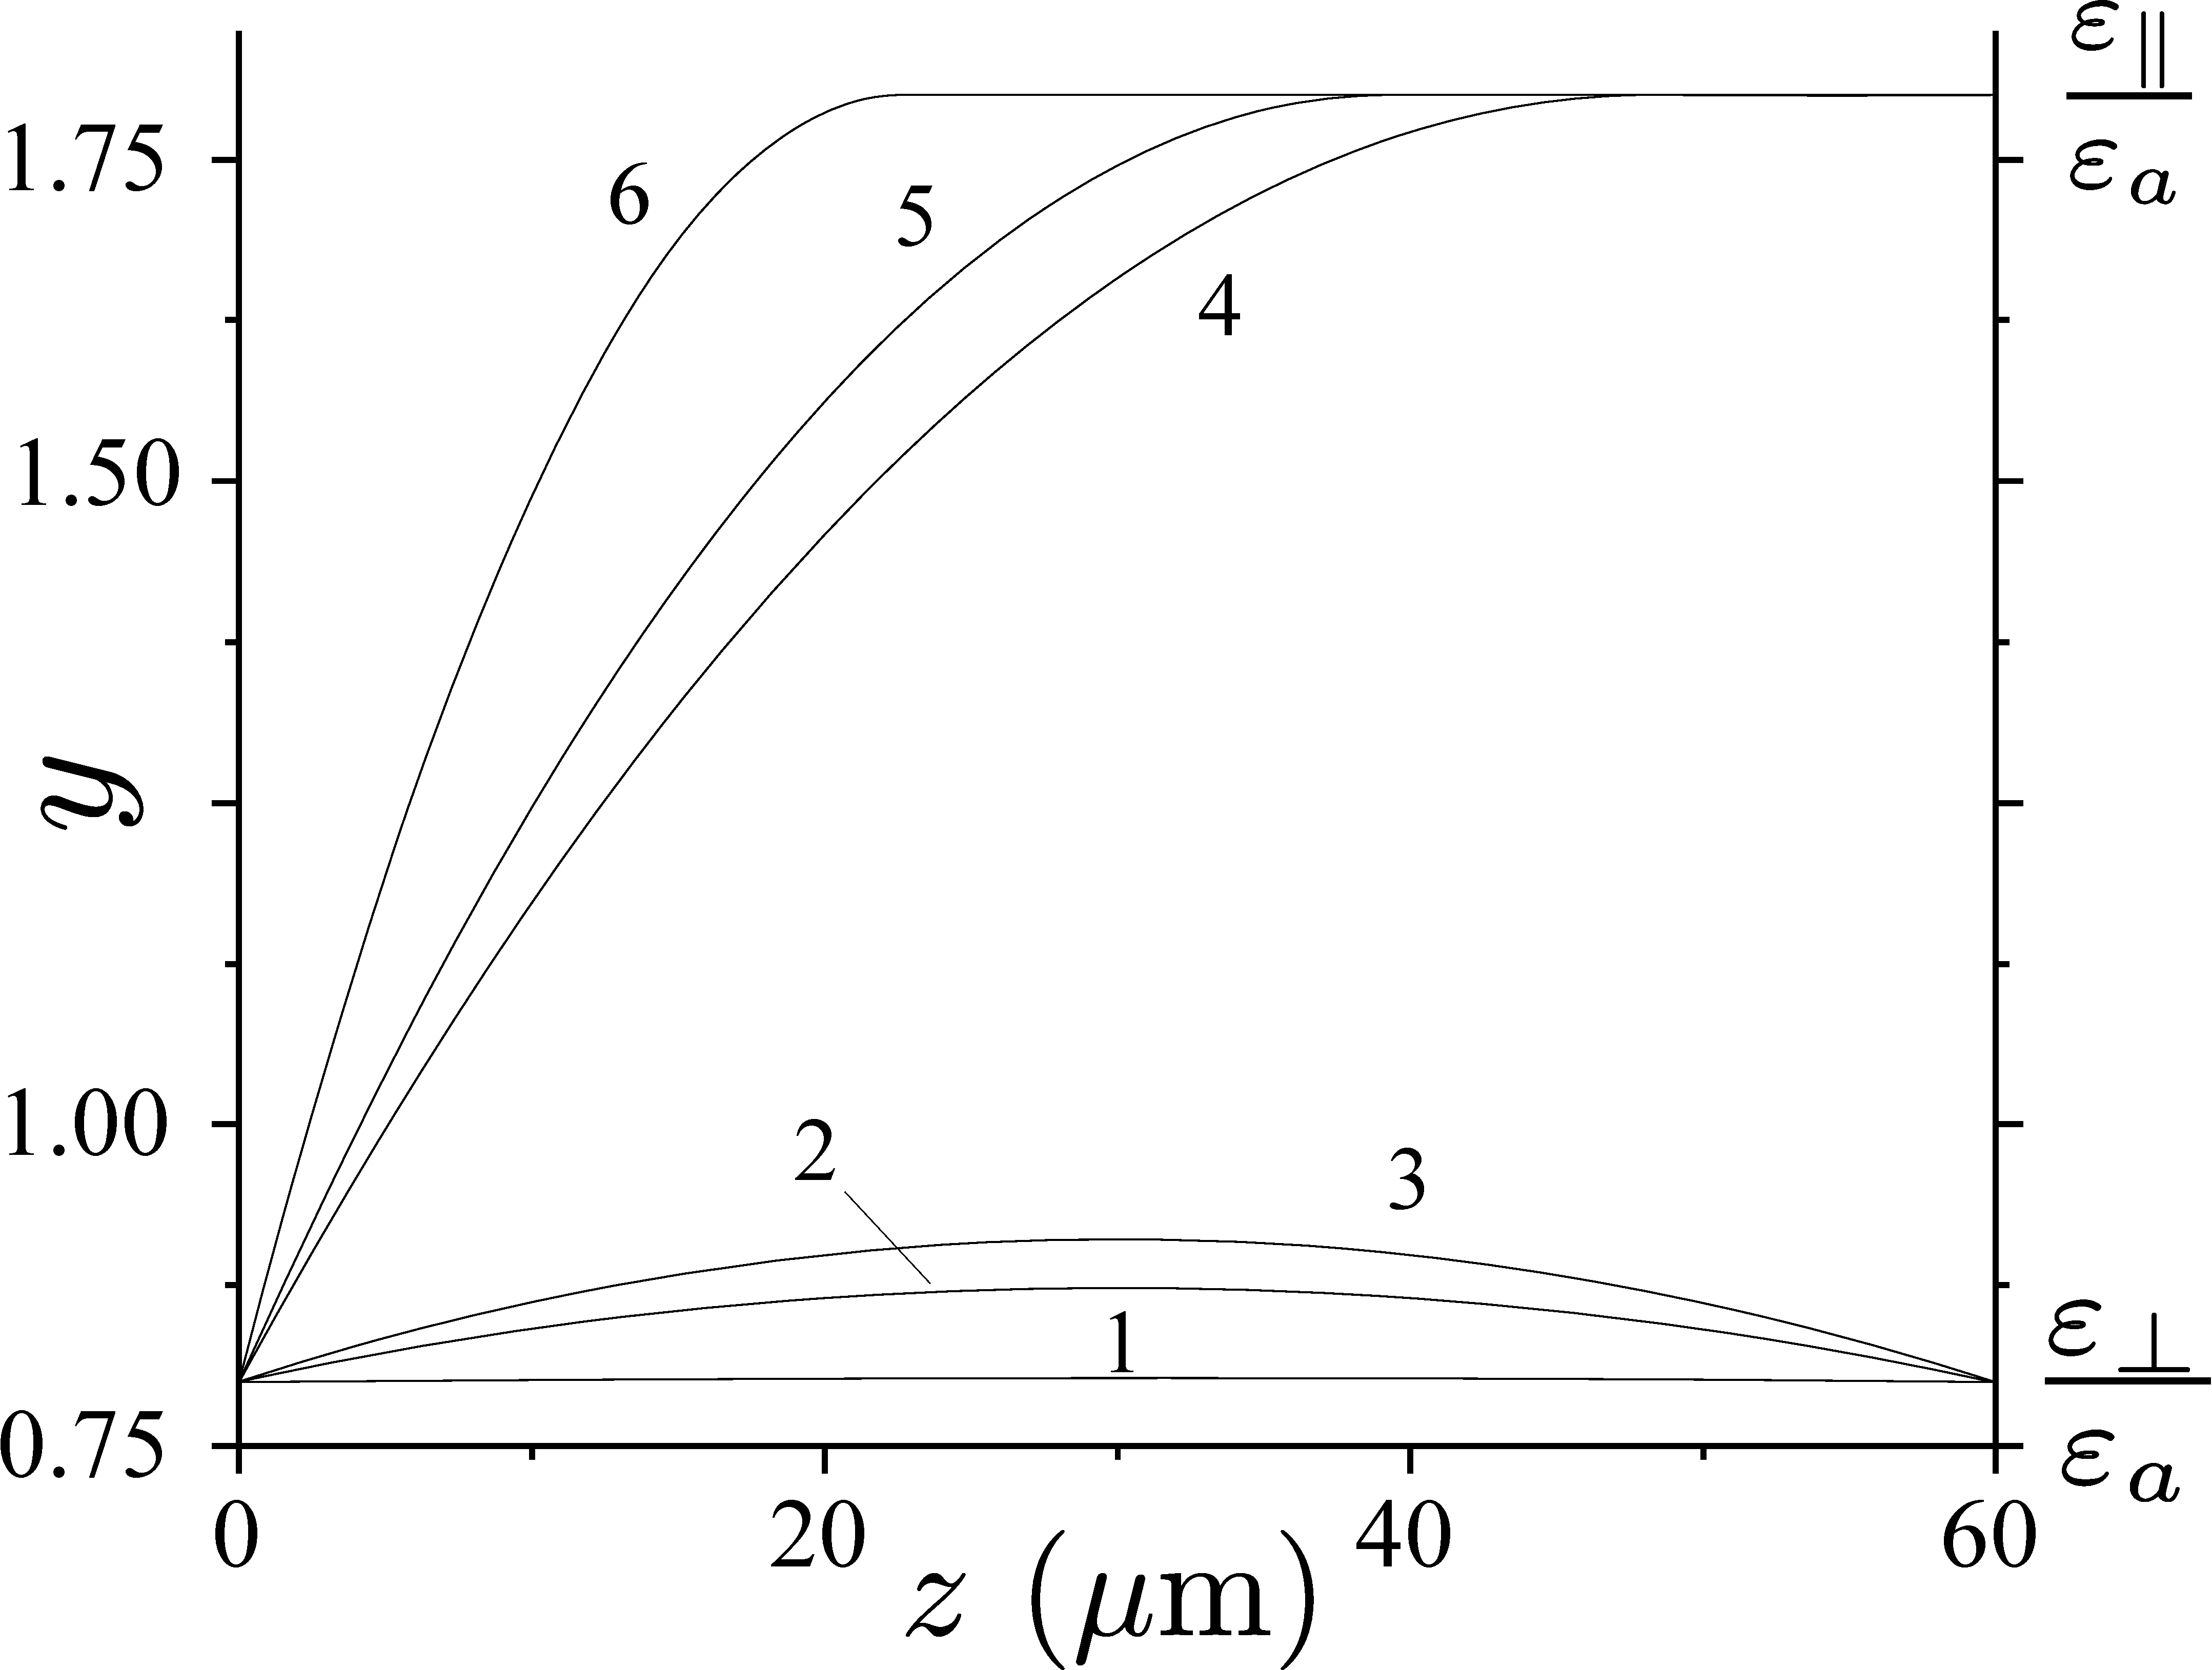
\includegraphics[width=0.49\textwidth]{Fig2_y_mid_anchoring.eps}
\caption{\footnotesize Профили $\theta(z)$ (слева) и зависимости $y(z)$ (справа), полученные для случая среднего зацепления, когда выполнено $4/(\varkappa - 1)> g_2 L > 2/\varkappa$. Модули поверхностного зацепления: $W_\theta^{(1)}=0.25\ \mathrm{erg}/\mathrm{cm}^2$, $W_\theta^{(2)} = 0.10\ \mathrm{erg}/\mathrm{cm}^2$ для всех кривых. Приложенное напряжение в соответствии с линиями: 1 -- $U = 1\,\mathrm{V}$, 2 -- $U = 5\,\mathrm{V}$, 3 -- $U = 6.1\,\mathrm{V}$, 4 -- $U = 6.2\,\mathrm{V}$, 5 -- $U = 8\,\mathrm{V}$, 6 -- $U = 15\,\mathrm{V}$.}
\end{figure}
\end{frame}


\begin{frame}
\frametitle{Большой $\bar{e}$ и высокое $U$}
\framesubtitle{Профили при сильном зацеплении}
\begin{figure}[ht]
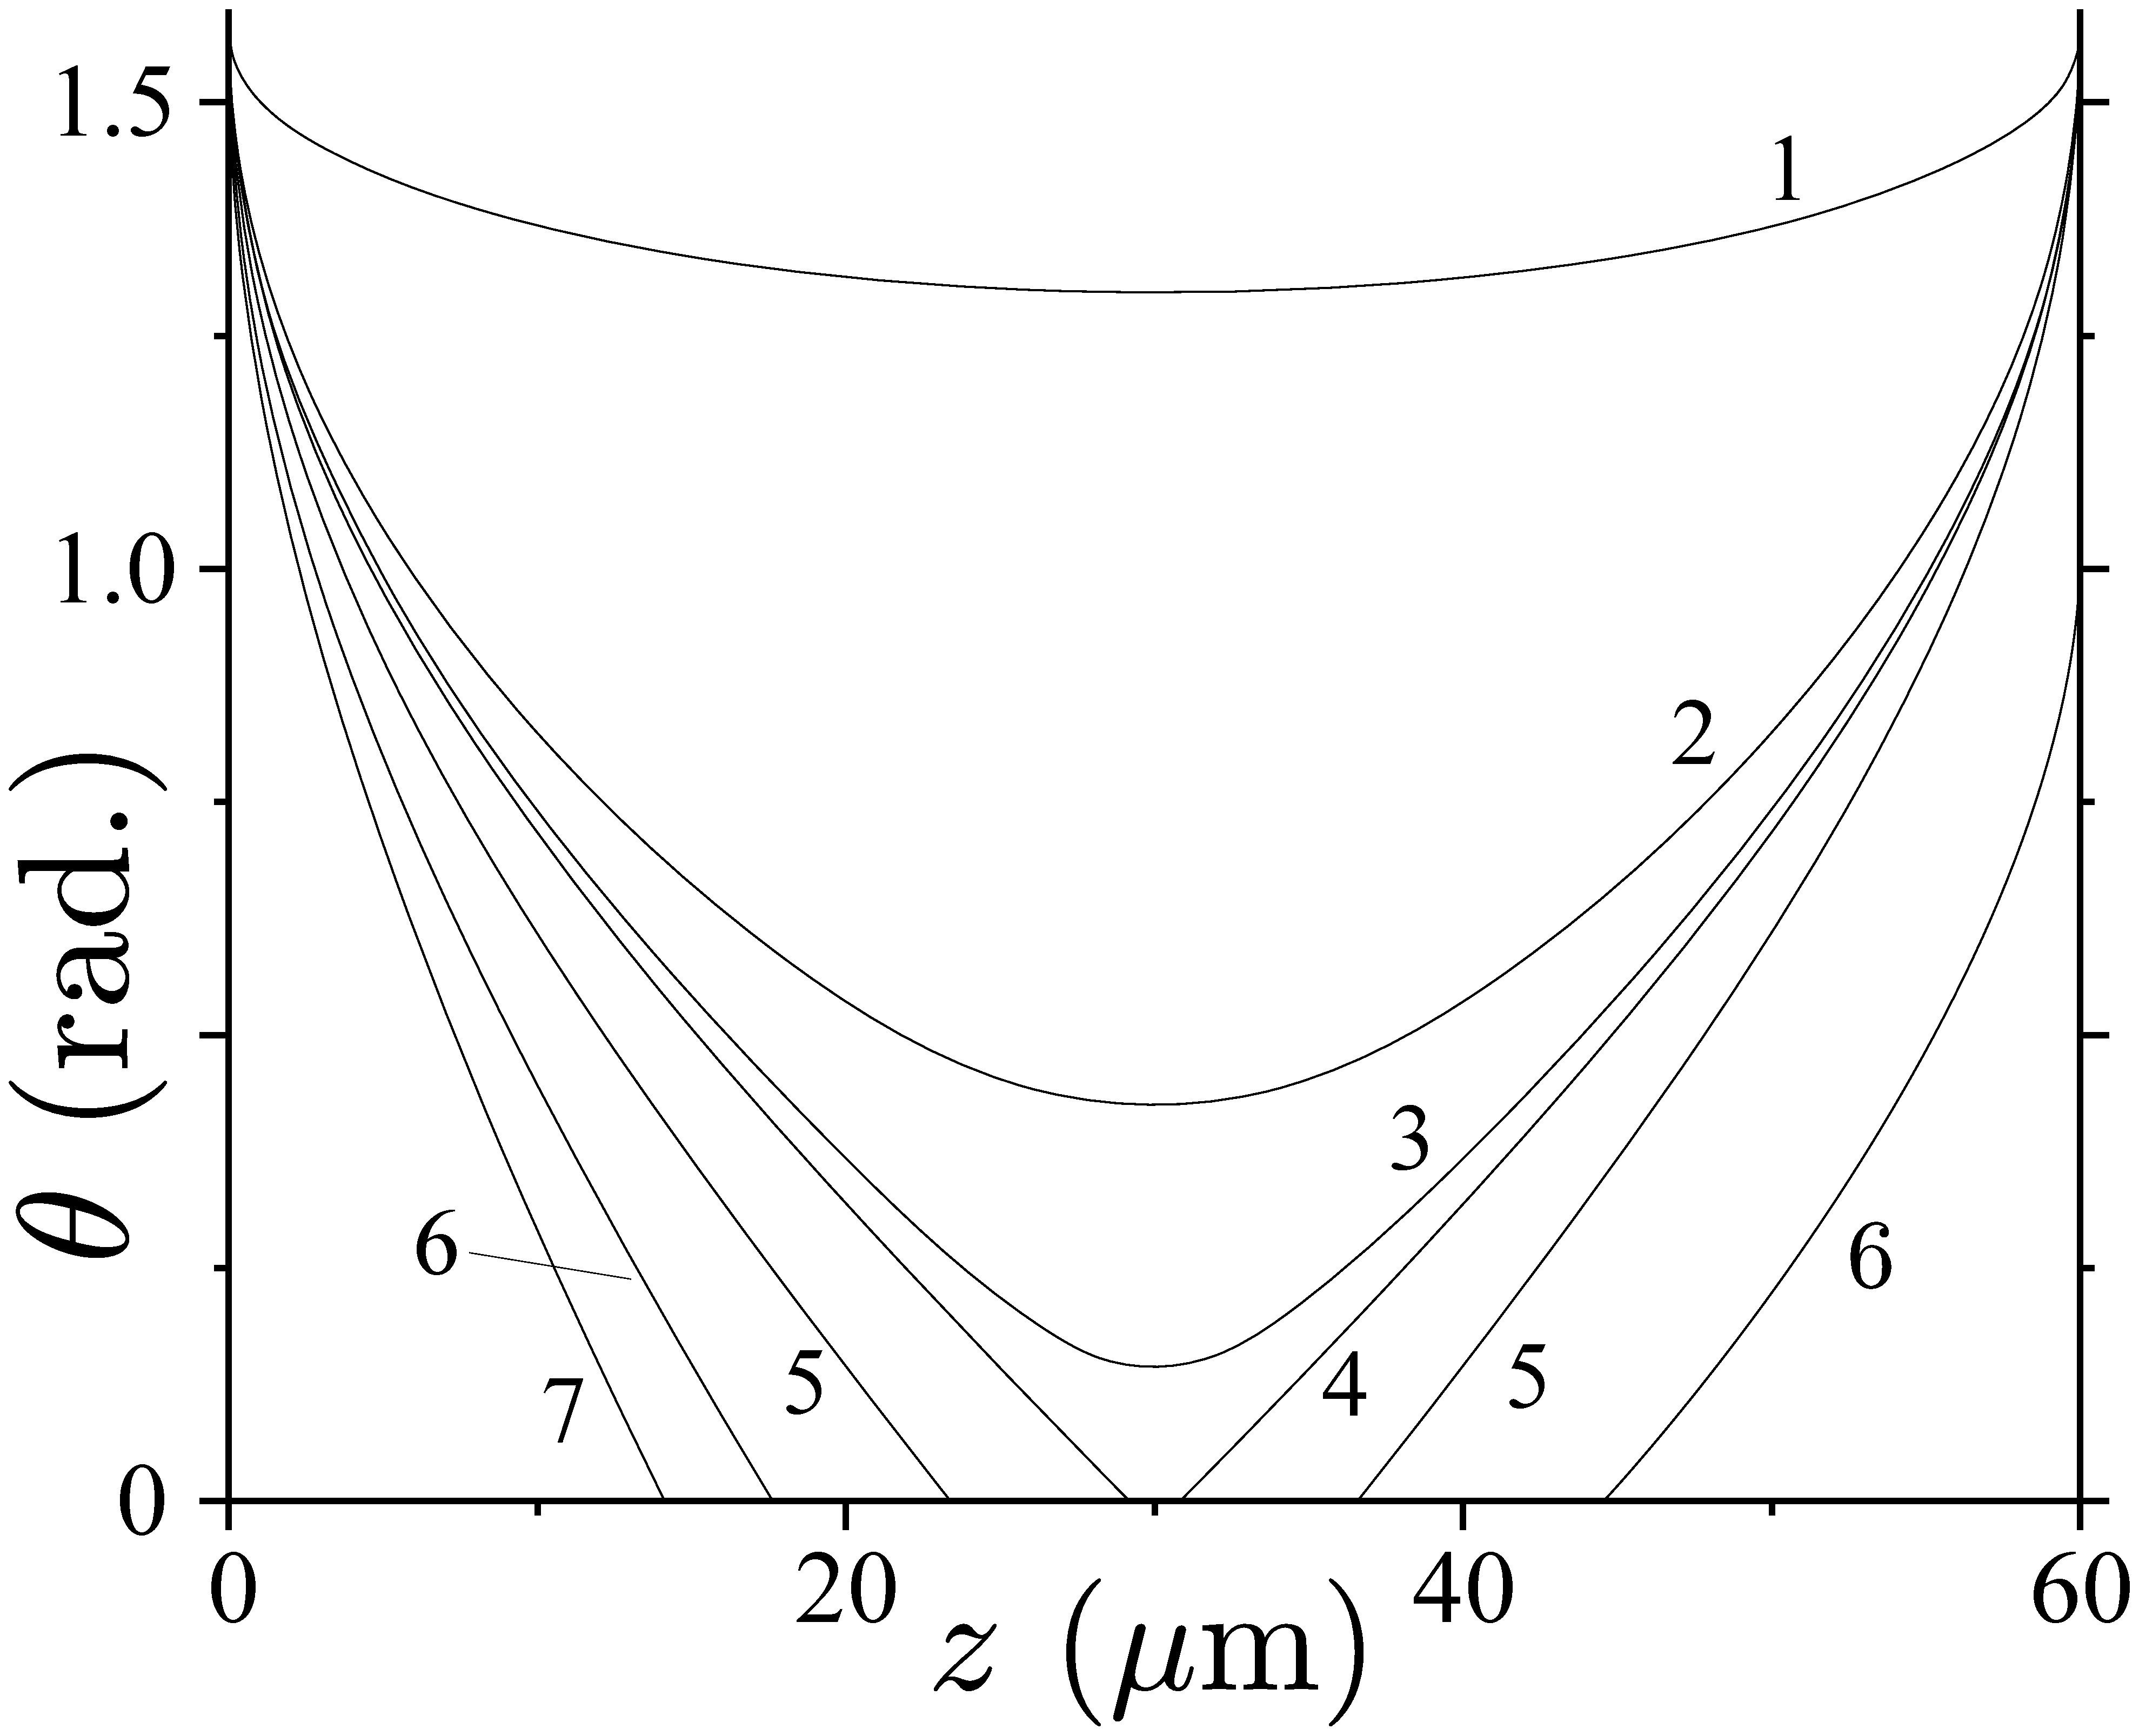
\includegraphics[width=0.45\textwidth]{Fig3_theta_high_anchoring.eps}%\hspace{2pc}%
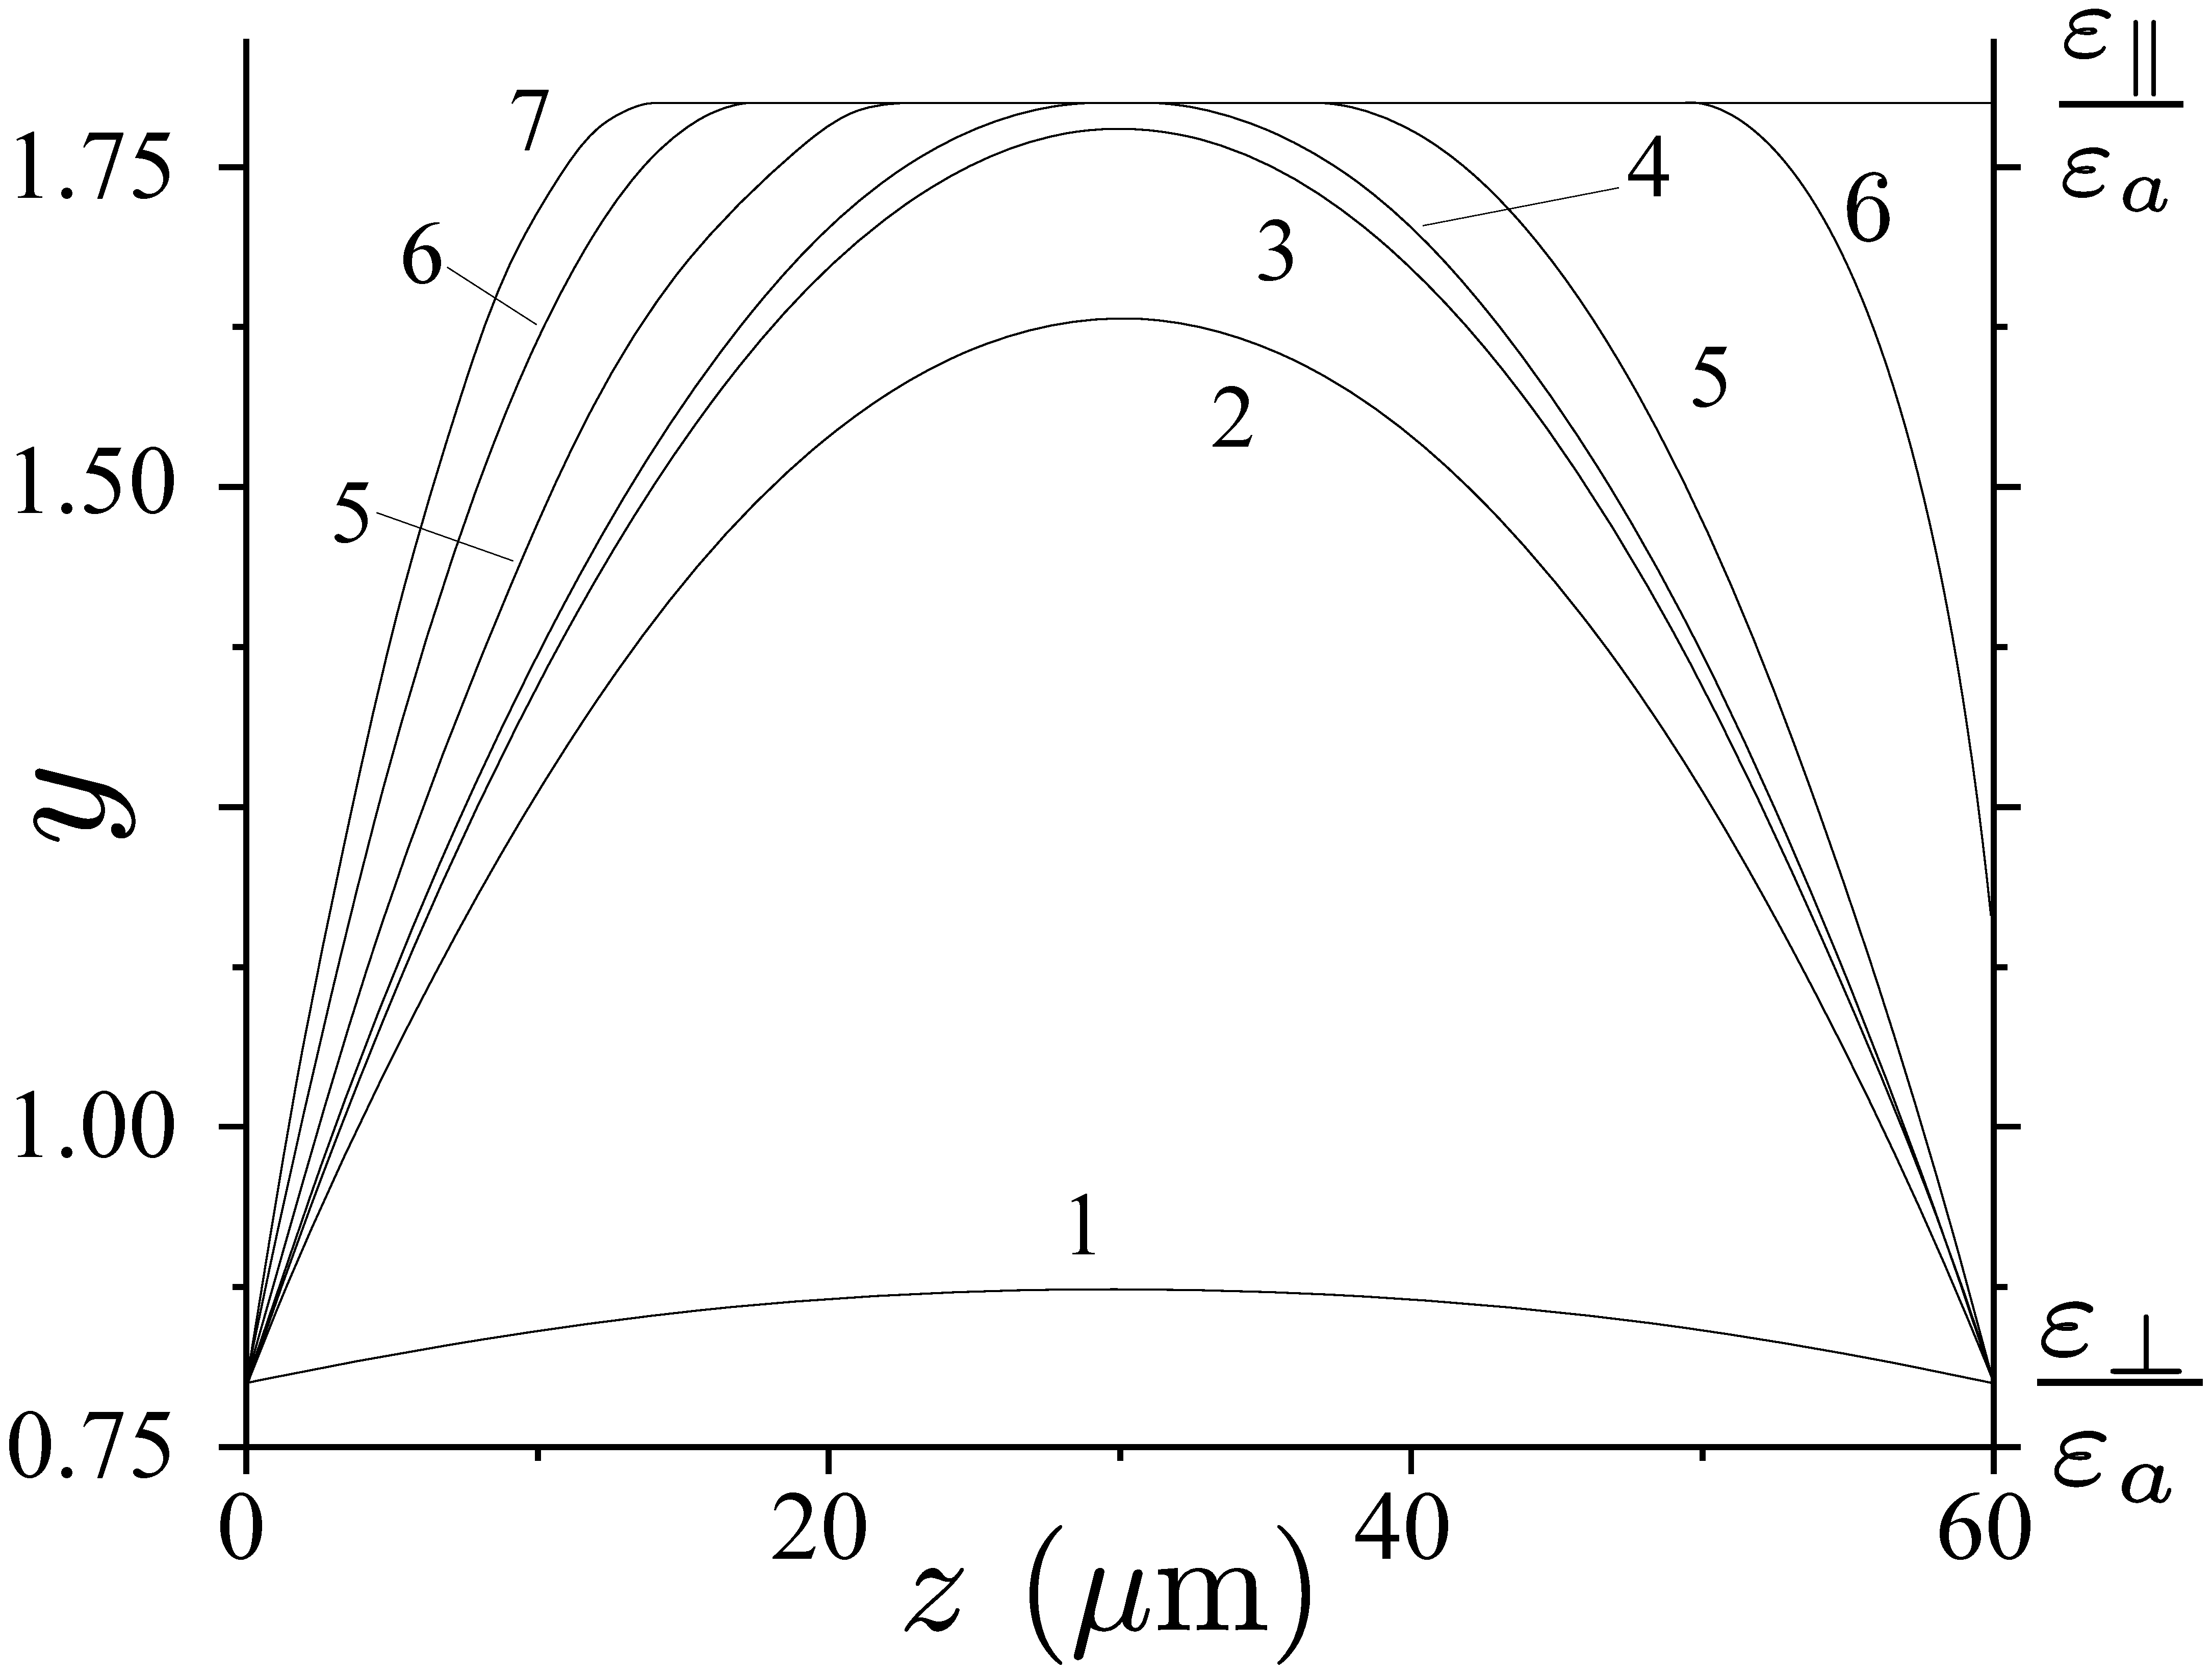
\includegraphics[width=0.49\textwidth]{Fig3_y_high_anchoring.eps}
\caption{ Профили $\theta(z)$ (слева) и зависимости $y(z)$ (справа), полученные для случая сильного зацепления, когда выполнено $4/(\varkappa - 1)< g_2 L$. Модули поверхностного зацепления: $W_\theta^{(1)}=1.75\ \mathrm{erg}/\mathrm{cm}^2$, $W_\theta^{(2)} = 0.7\ \mathrm{erg}/\mathrm{cm}^2$ для всех кривых. Приложенное напряжение в соответствии с линиями: 1 -- $U = 5\,\mathrm{V}$, 2 -- $U = 15\,\mathrm{V}$, 3 -- $U = 16\,\mathrm{V}$, 4 -- $U = 16.5\,\mathrm{V}$, 5 -- $U = 19.65\,\mathrm{V}$, 6 -- $U = 19.75\,\mathrm{V}$, 7 -- $U = 65\,\mathrm{V}$.}
\end{figure}
\end{frame}


\begin{frame}
\frametitle{Основные результаты}
%\framesubtitle{Сравнение прямой минимизации и аналитической}
\begin{enumerate}
\item Для случая большого флексоэлектрического коэффициента, немалого $U$ и $\varepsilon_a > 0$ аналитически расчитаны профили $\theta(z)$;
\item Показано, как изменяется эволючия профилей $\theta(z)$ с изменением $U$ в зависимости материальных параметров
\end{enumerate}
\end{frame}

%\begin{frame}
%\frametitle{Выводы}
%\begin{itemize}
%\item В ходе работы объяснена немонотонность гравика зависимости $U^{*}(\overline{e}_{13})$;
%\item Найден способ анализа рода характера перехода Фредерикса при заданных параметрах системы.
%\item Реализована процедура моделирования динамики
%\item Построены графики зависимостей напряжений $U^*$, $U_c$, $U^{**}$, характеризующих переход Фредерикса, от $%\overline{e}_{13}$;
%\item Получен критерий устойчивости планарной геликоидальной структуры;

%\end{itemize}
%\end{frame}


\end{document} 